\subsection{External Interface Requirements}

\subsubsection{User Interfaces}


In this section, we present user interfaces for Students and Educators. We created a detailed user interface design to inform the reader from a broader perspective. 
\begin{center}
    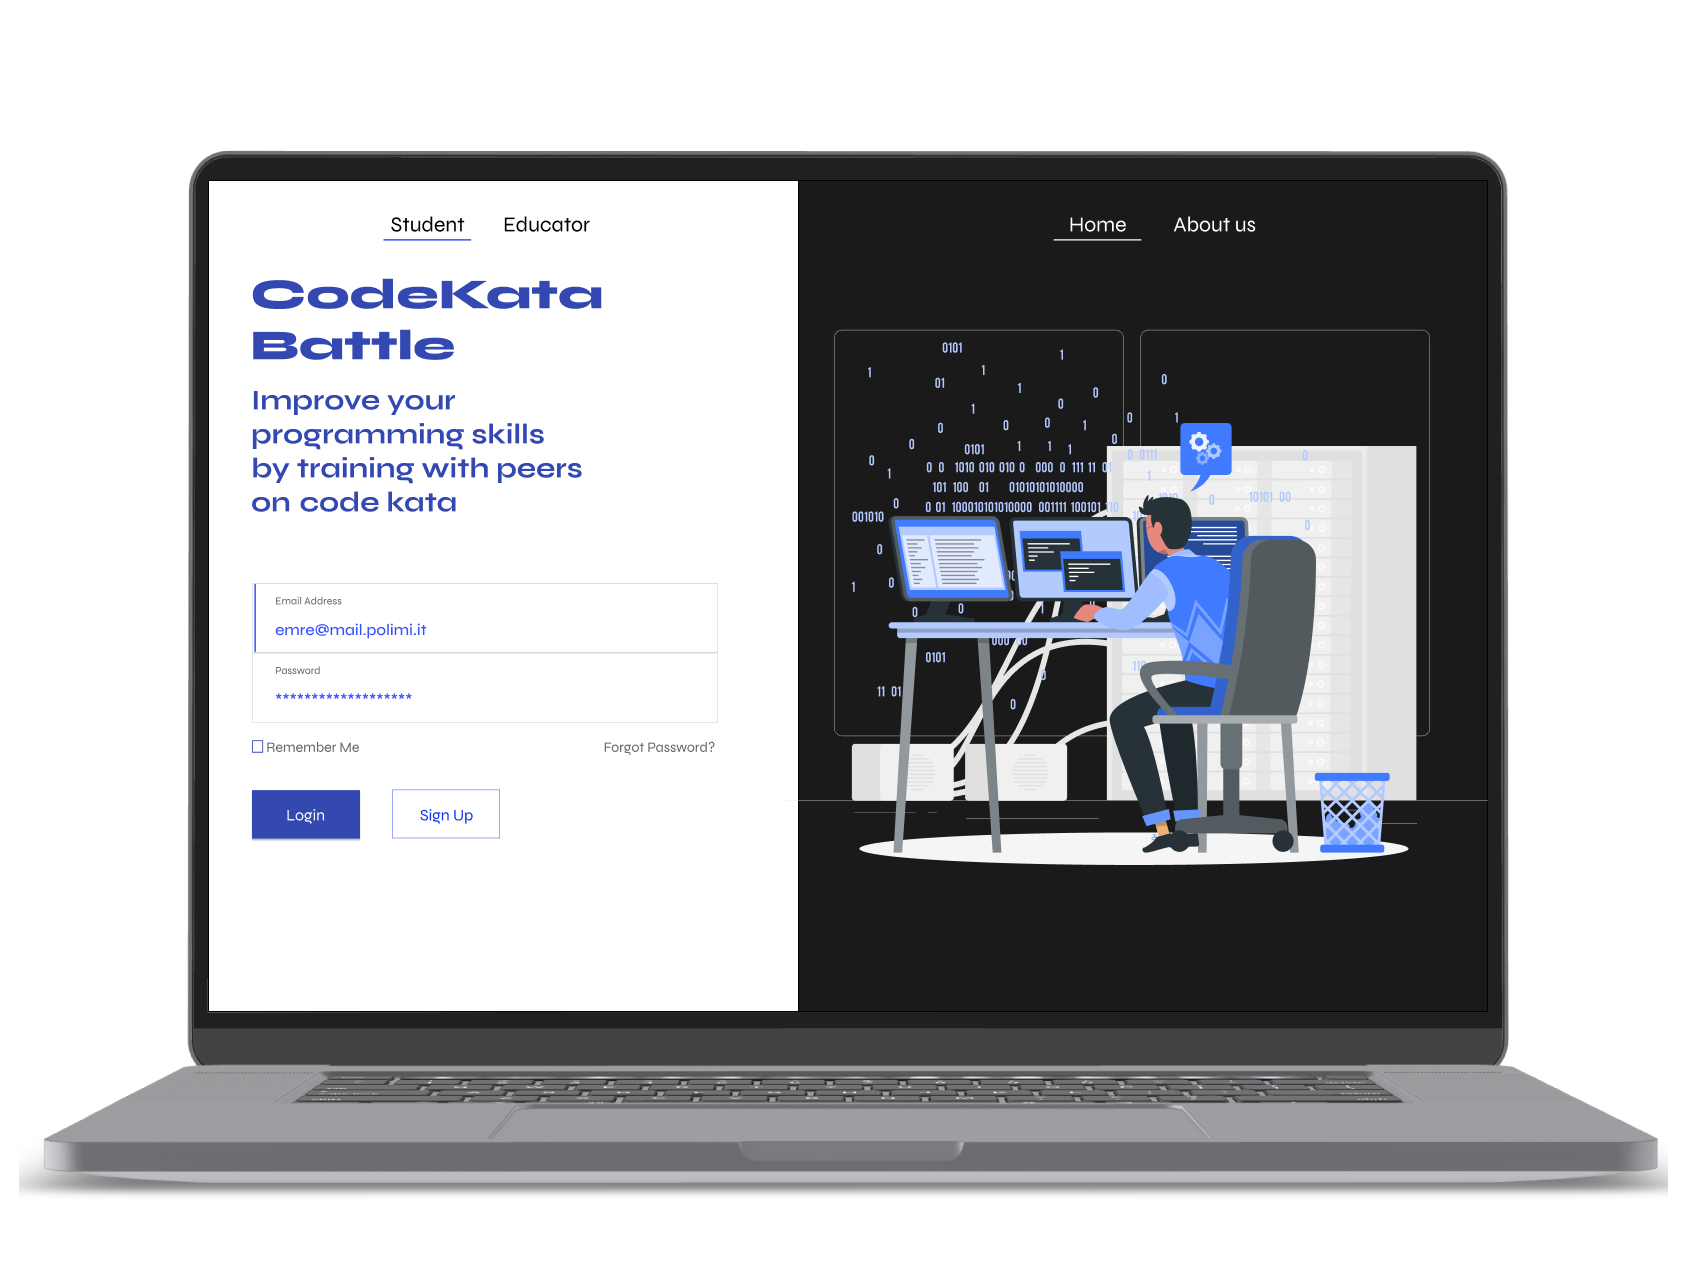
\includegraphics[scale=0.13]{Images/ui-ux/login-signup/student_login.png}
    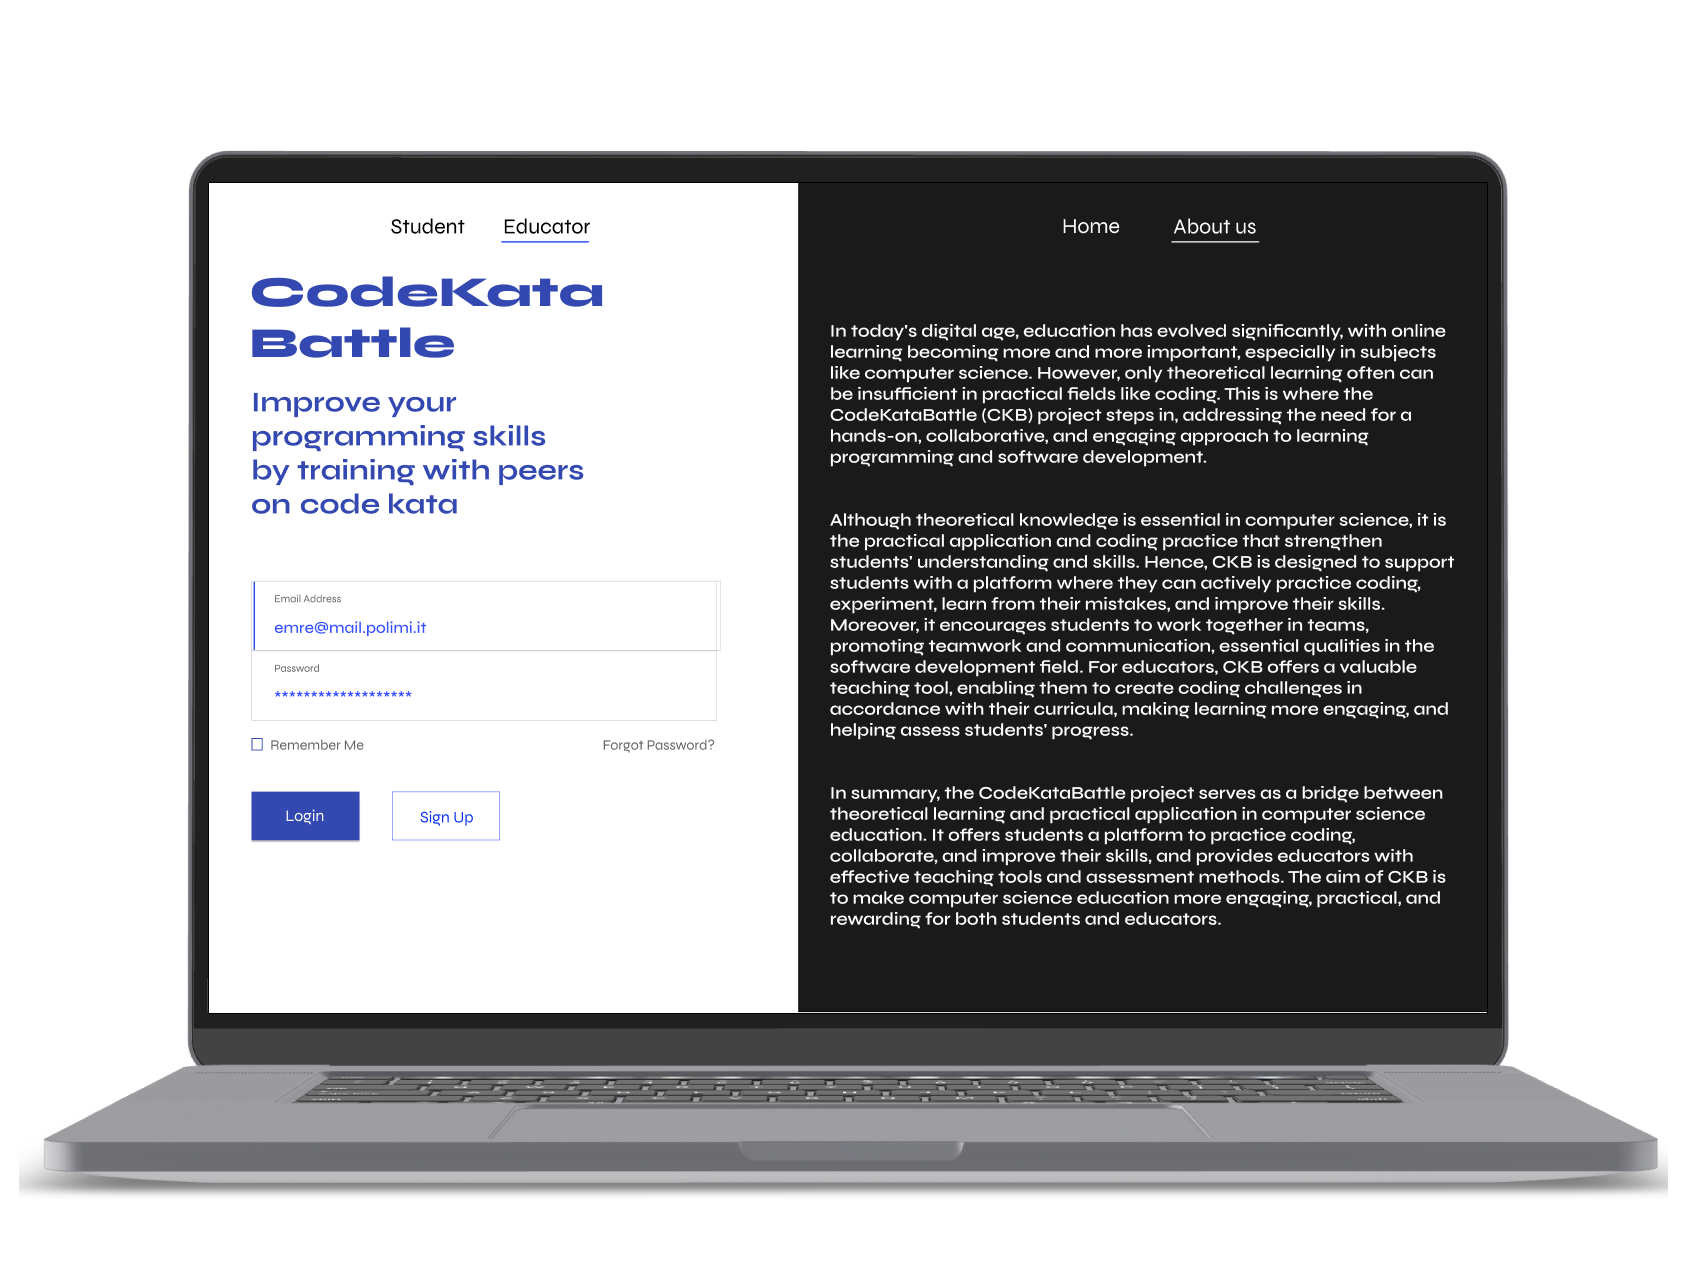
\includegraphics[scale=0.13]{Images/ui-ux/login-signup/educator_login.png}
\end{center}
    \begin{center}
        (a) Login Screens
    \end{center}
\begin{center}
    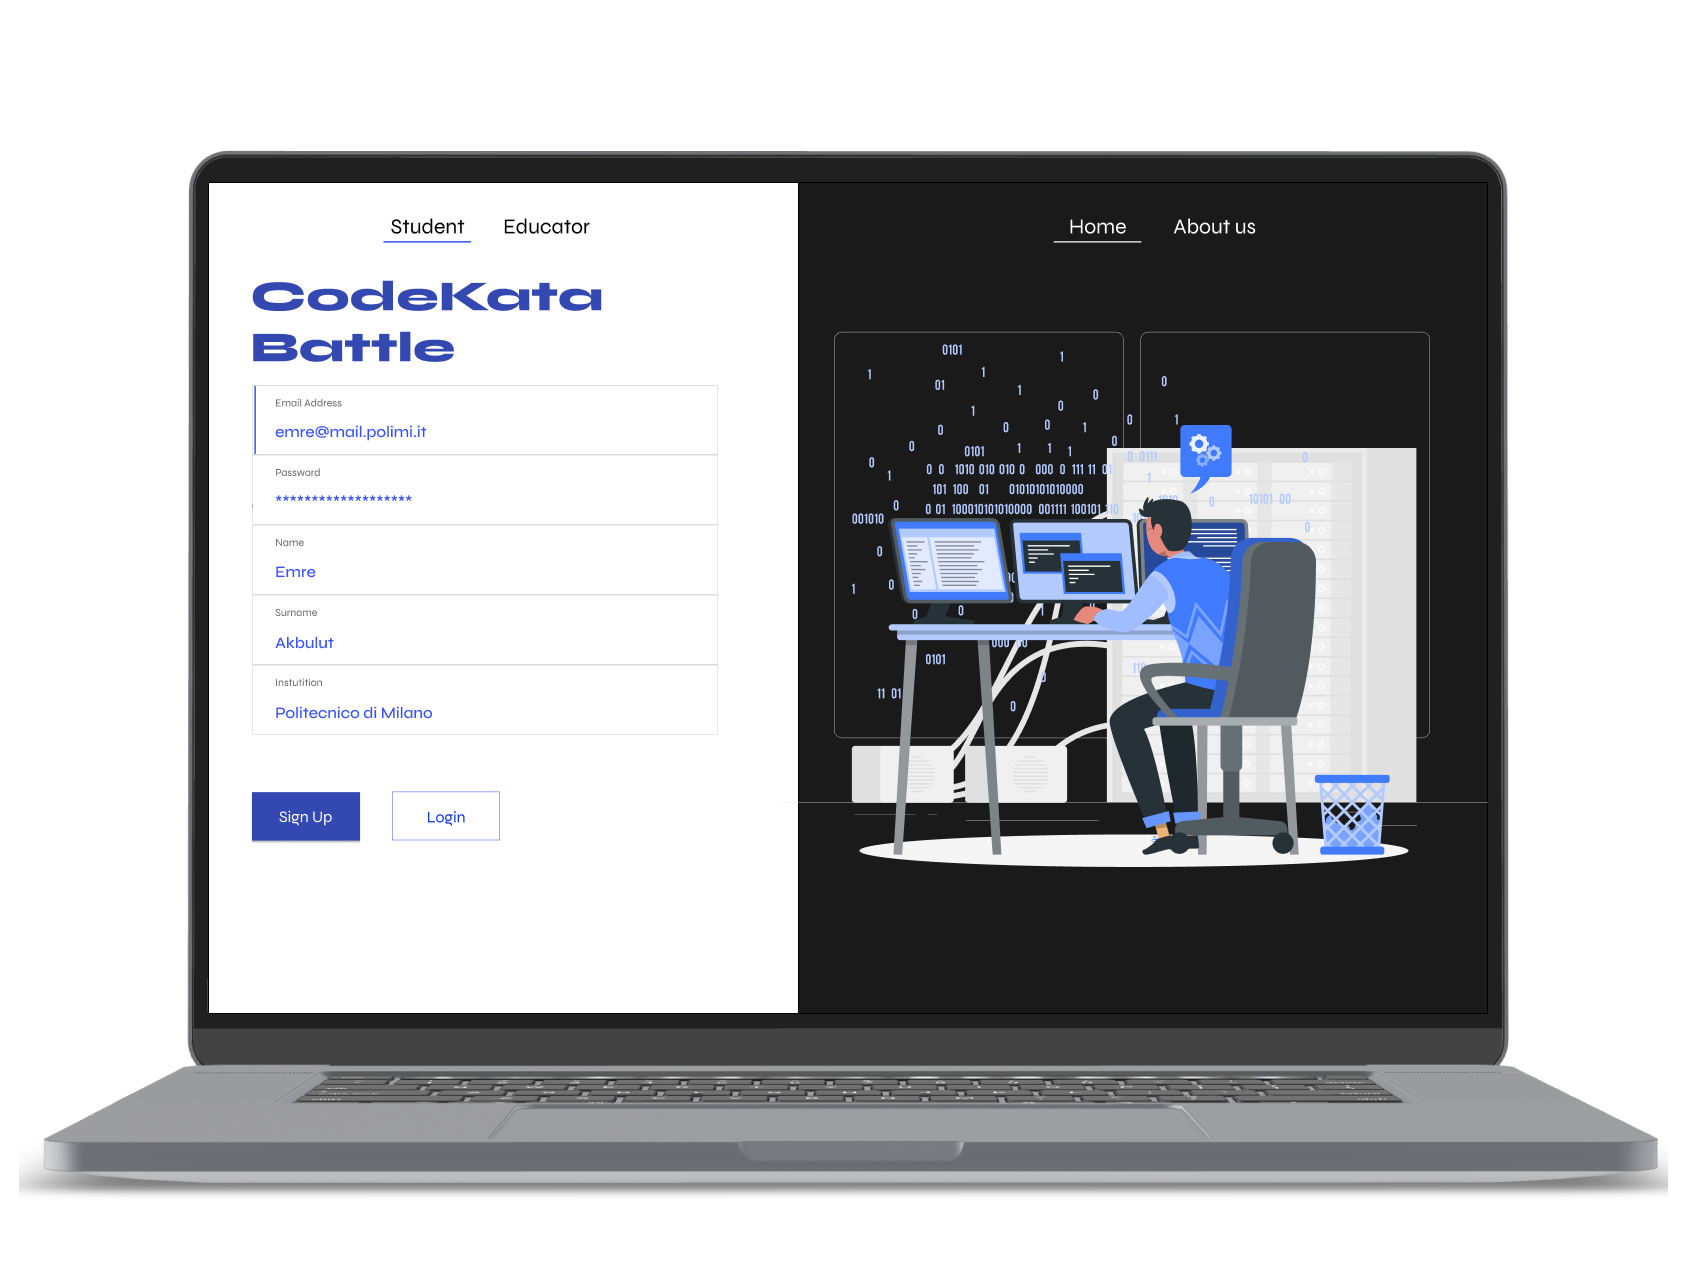
\includegraphics[scale=0.13]{Images/ui-ux/login-signup/student_signup.png}
    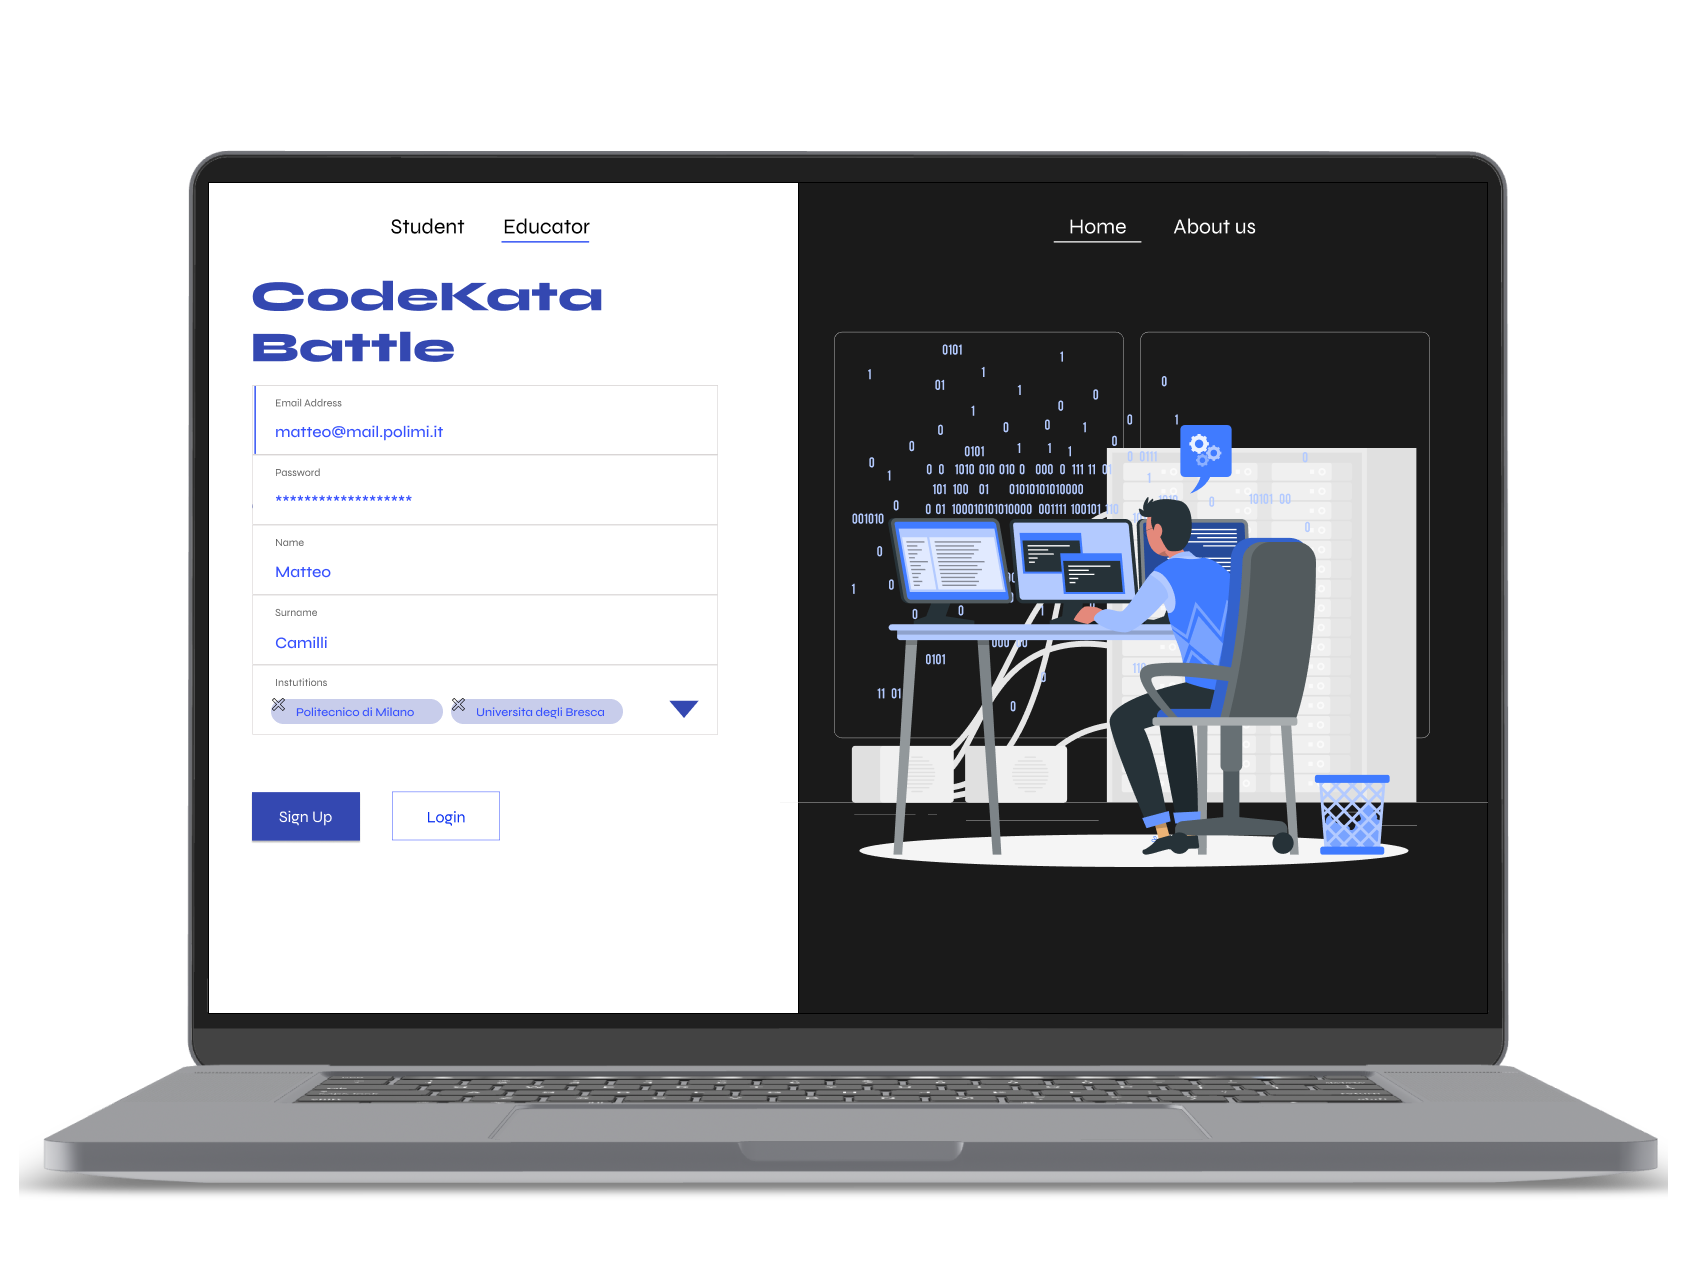
\includegraphics[scale=0.13]{Images/ui-ux/login-signup/educator_signup.png}
    (b) Sign up Screens
\end{center}
\newpage
\begin{center}
    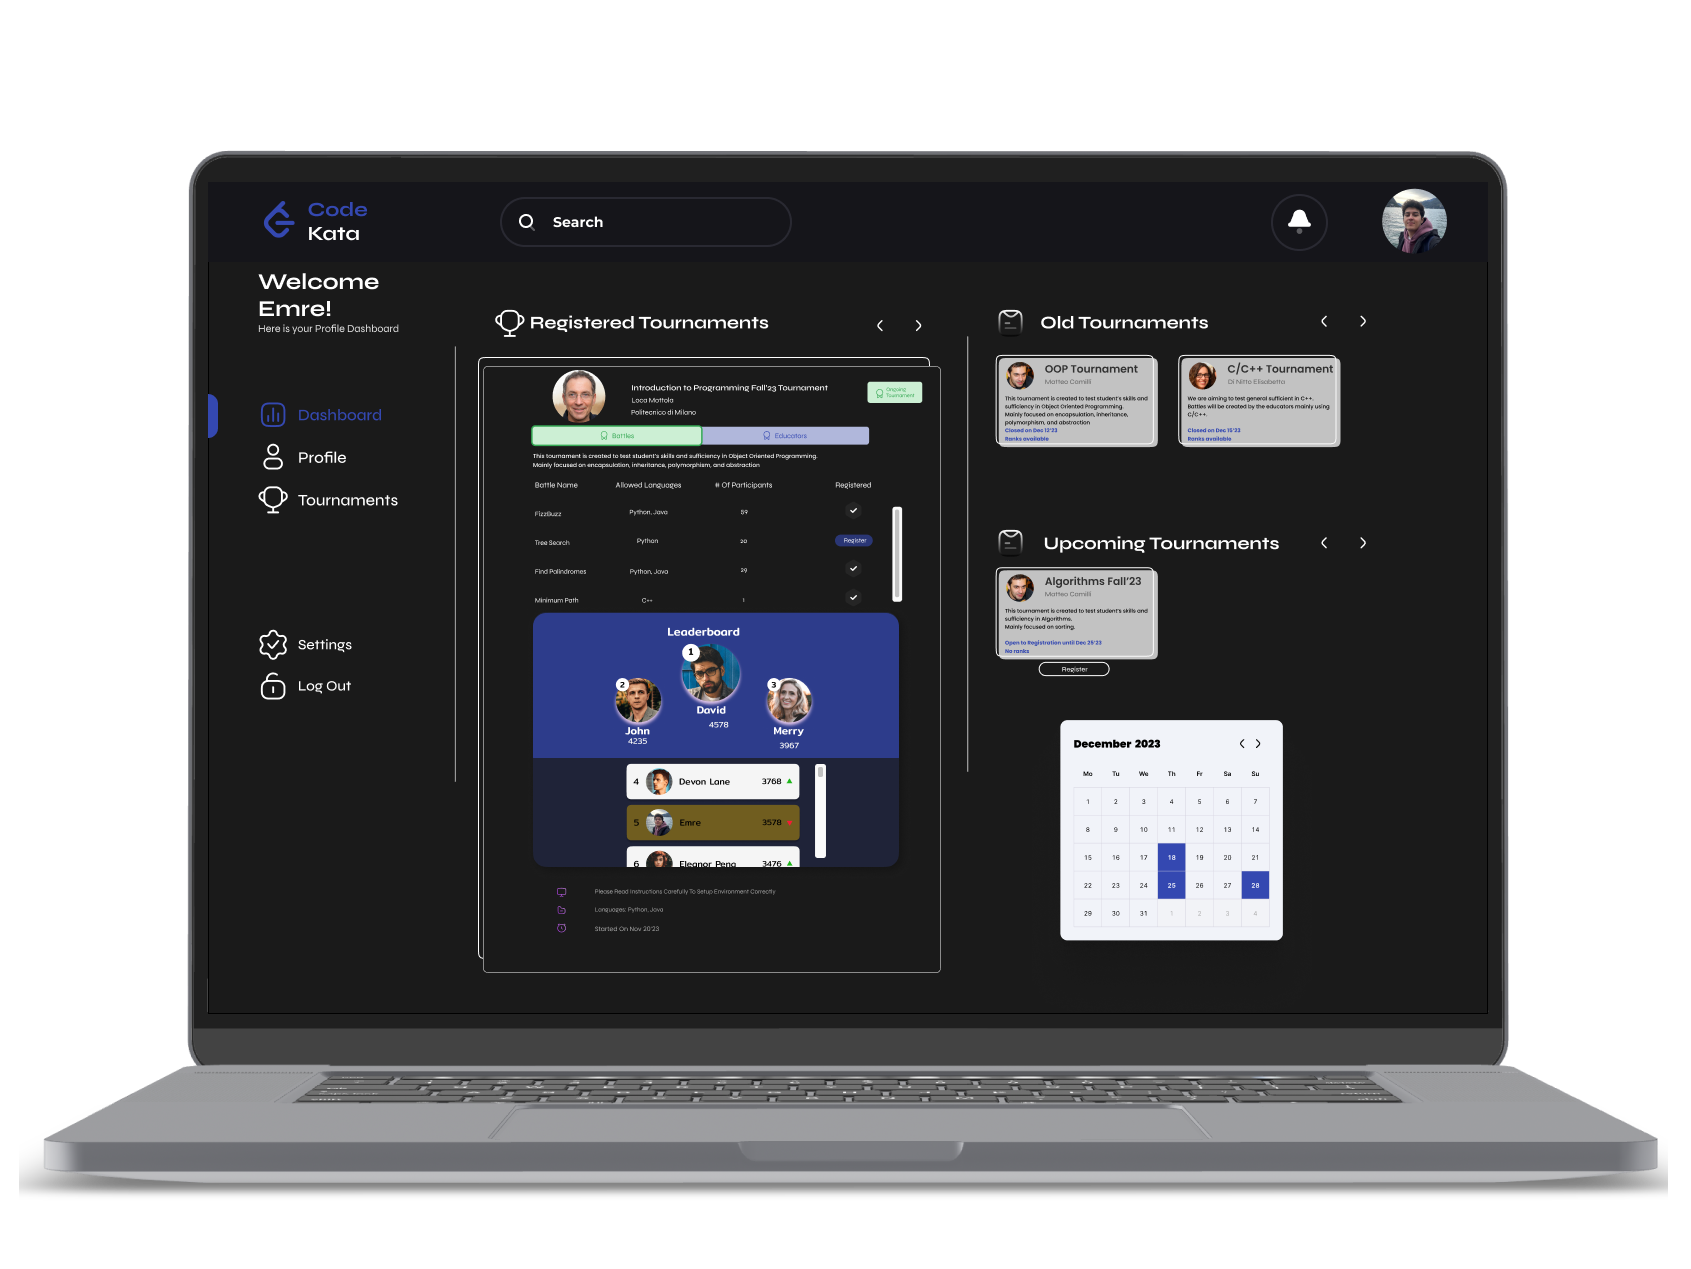
\includegraphics[scale=0.13]{Images/ui-ux/student_dashboard/student_dashboard_1.png}
    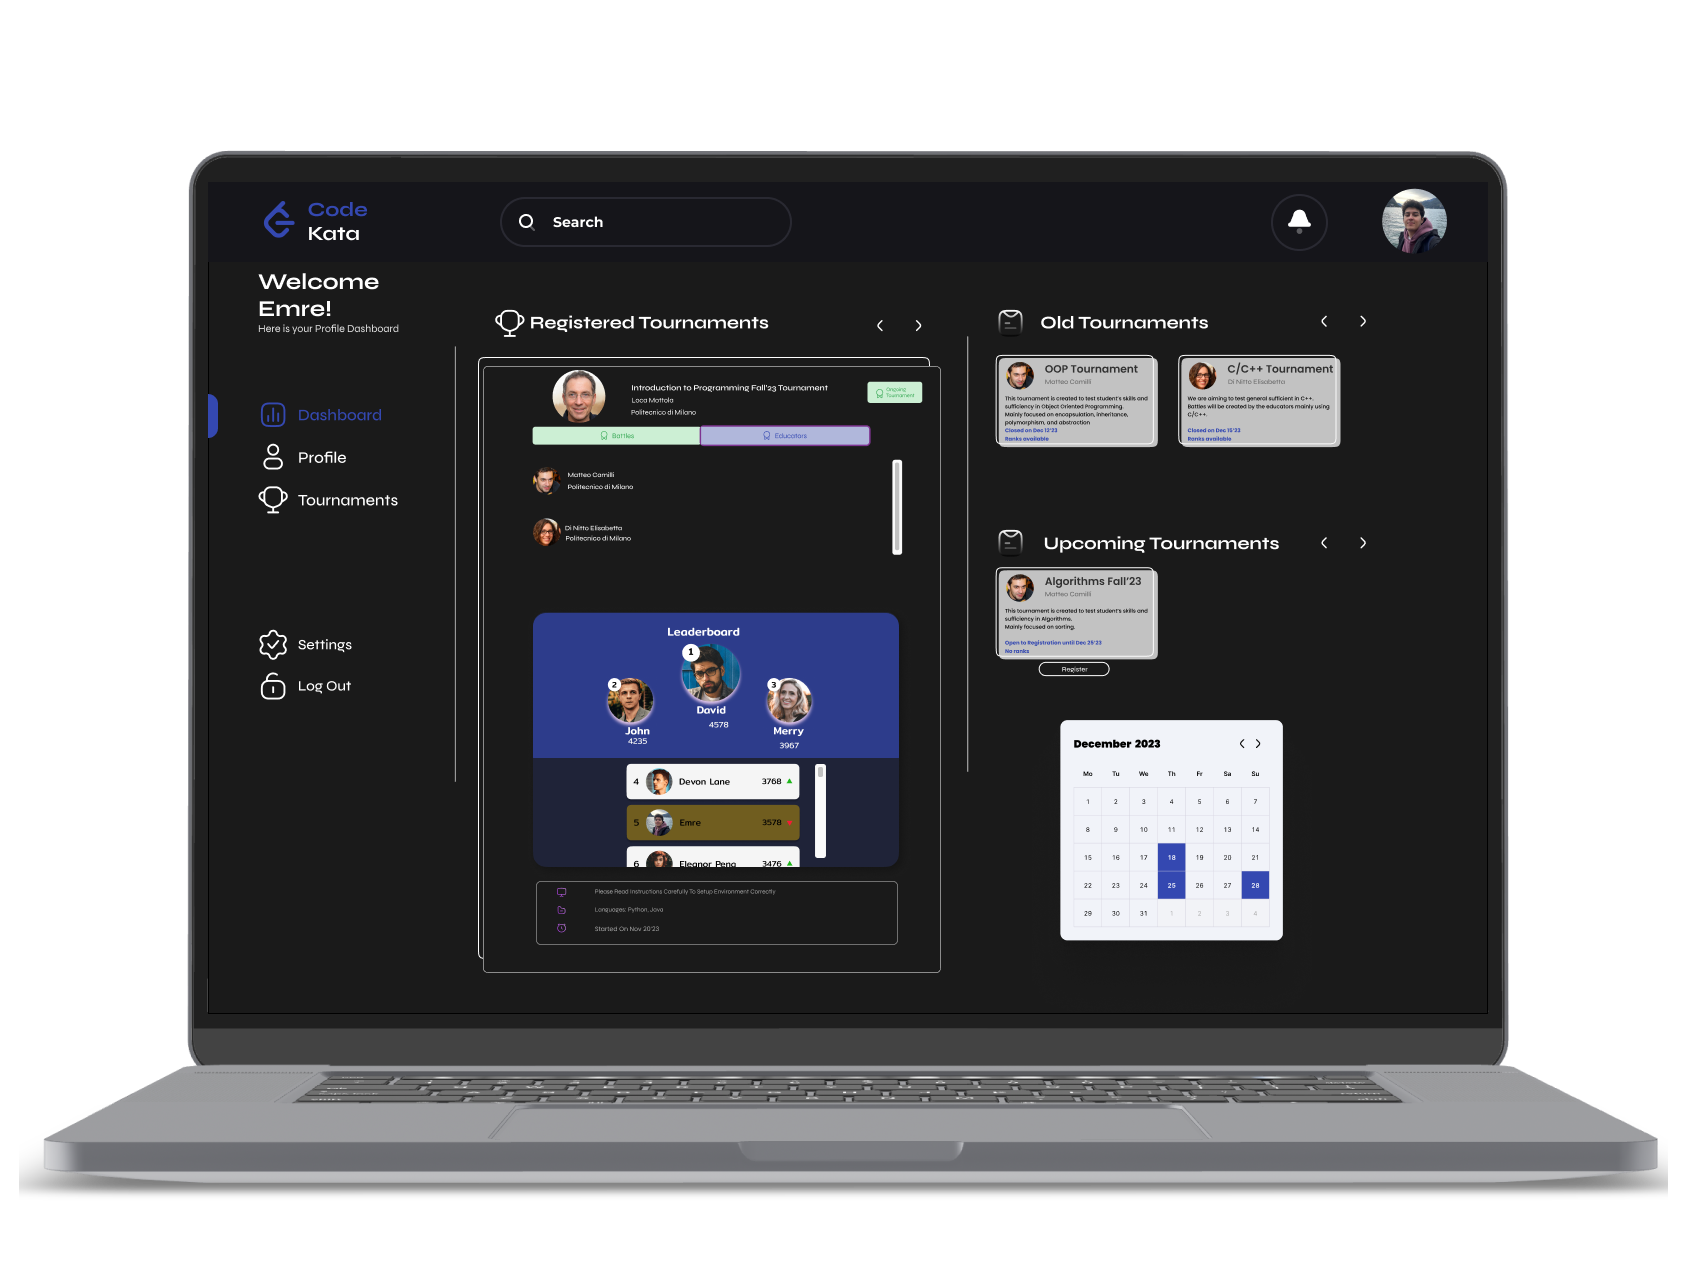
\includegraphics[scale=0.13]{Images/ui-ux/student_dashboard/student_dashboard_2.png}
            (c) Student Dashboard
\end{center}
\begin{center}
    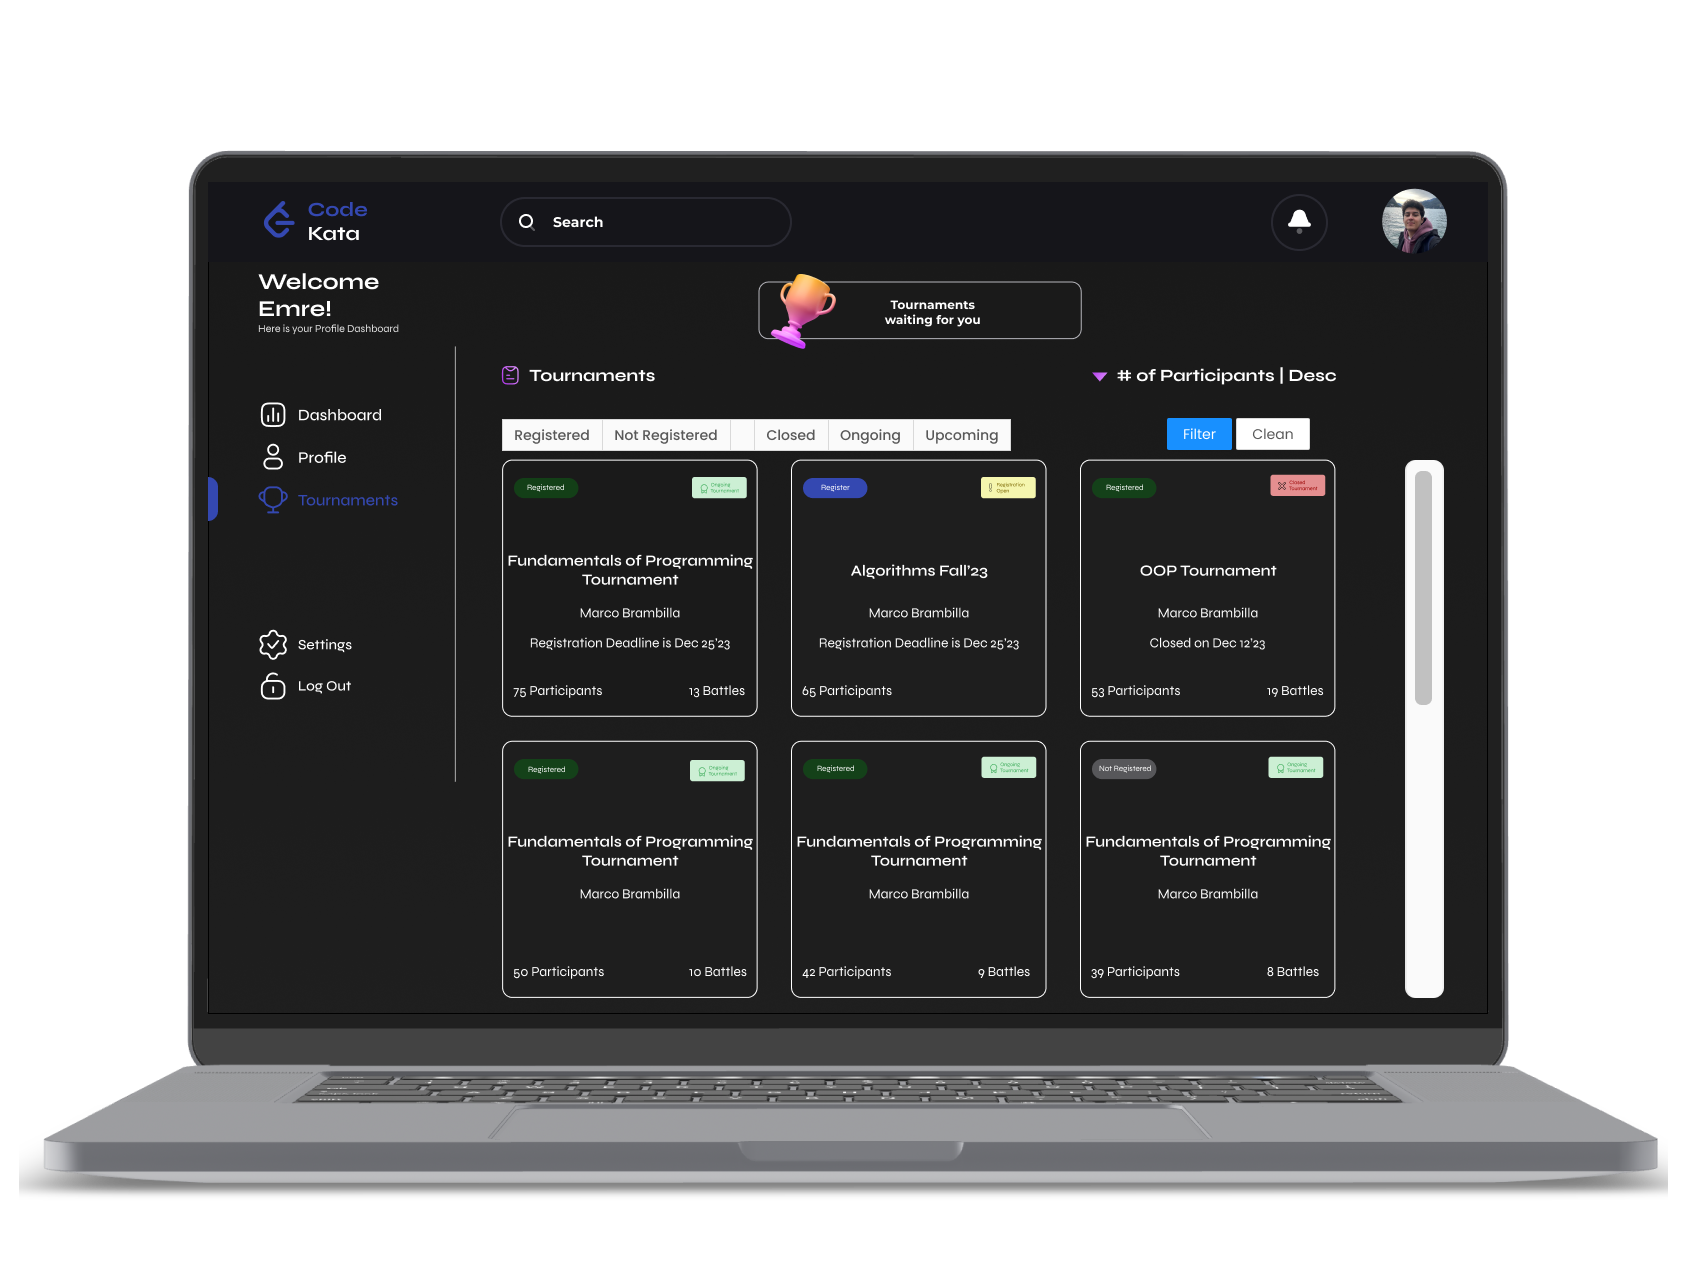
\includegraphics[scale=0.13]{Images/ui-ux/student_tournaments/student_tournaments_1.png}
    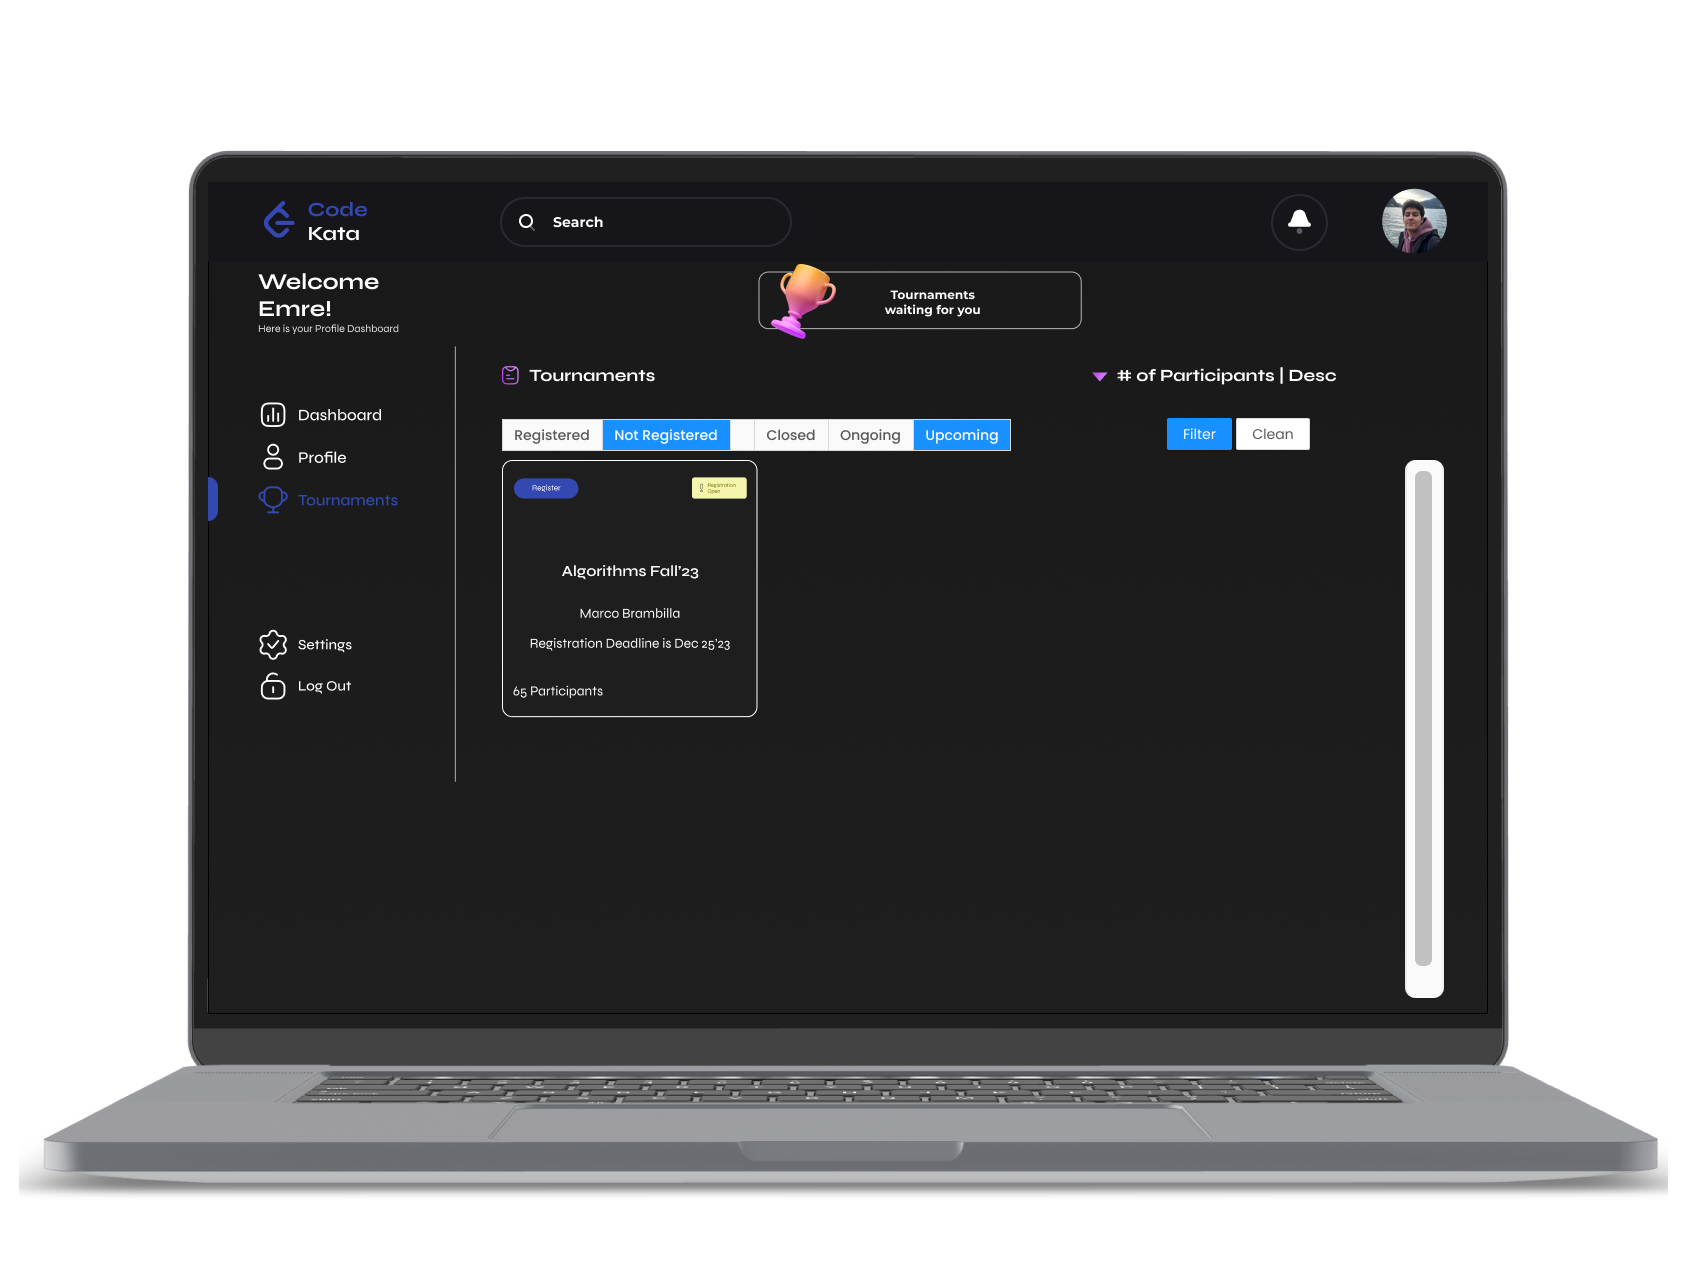
\includegraphics[scale=0.13]{Images/ui-ux/student_tournaments/student_tournaments_2.png}    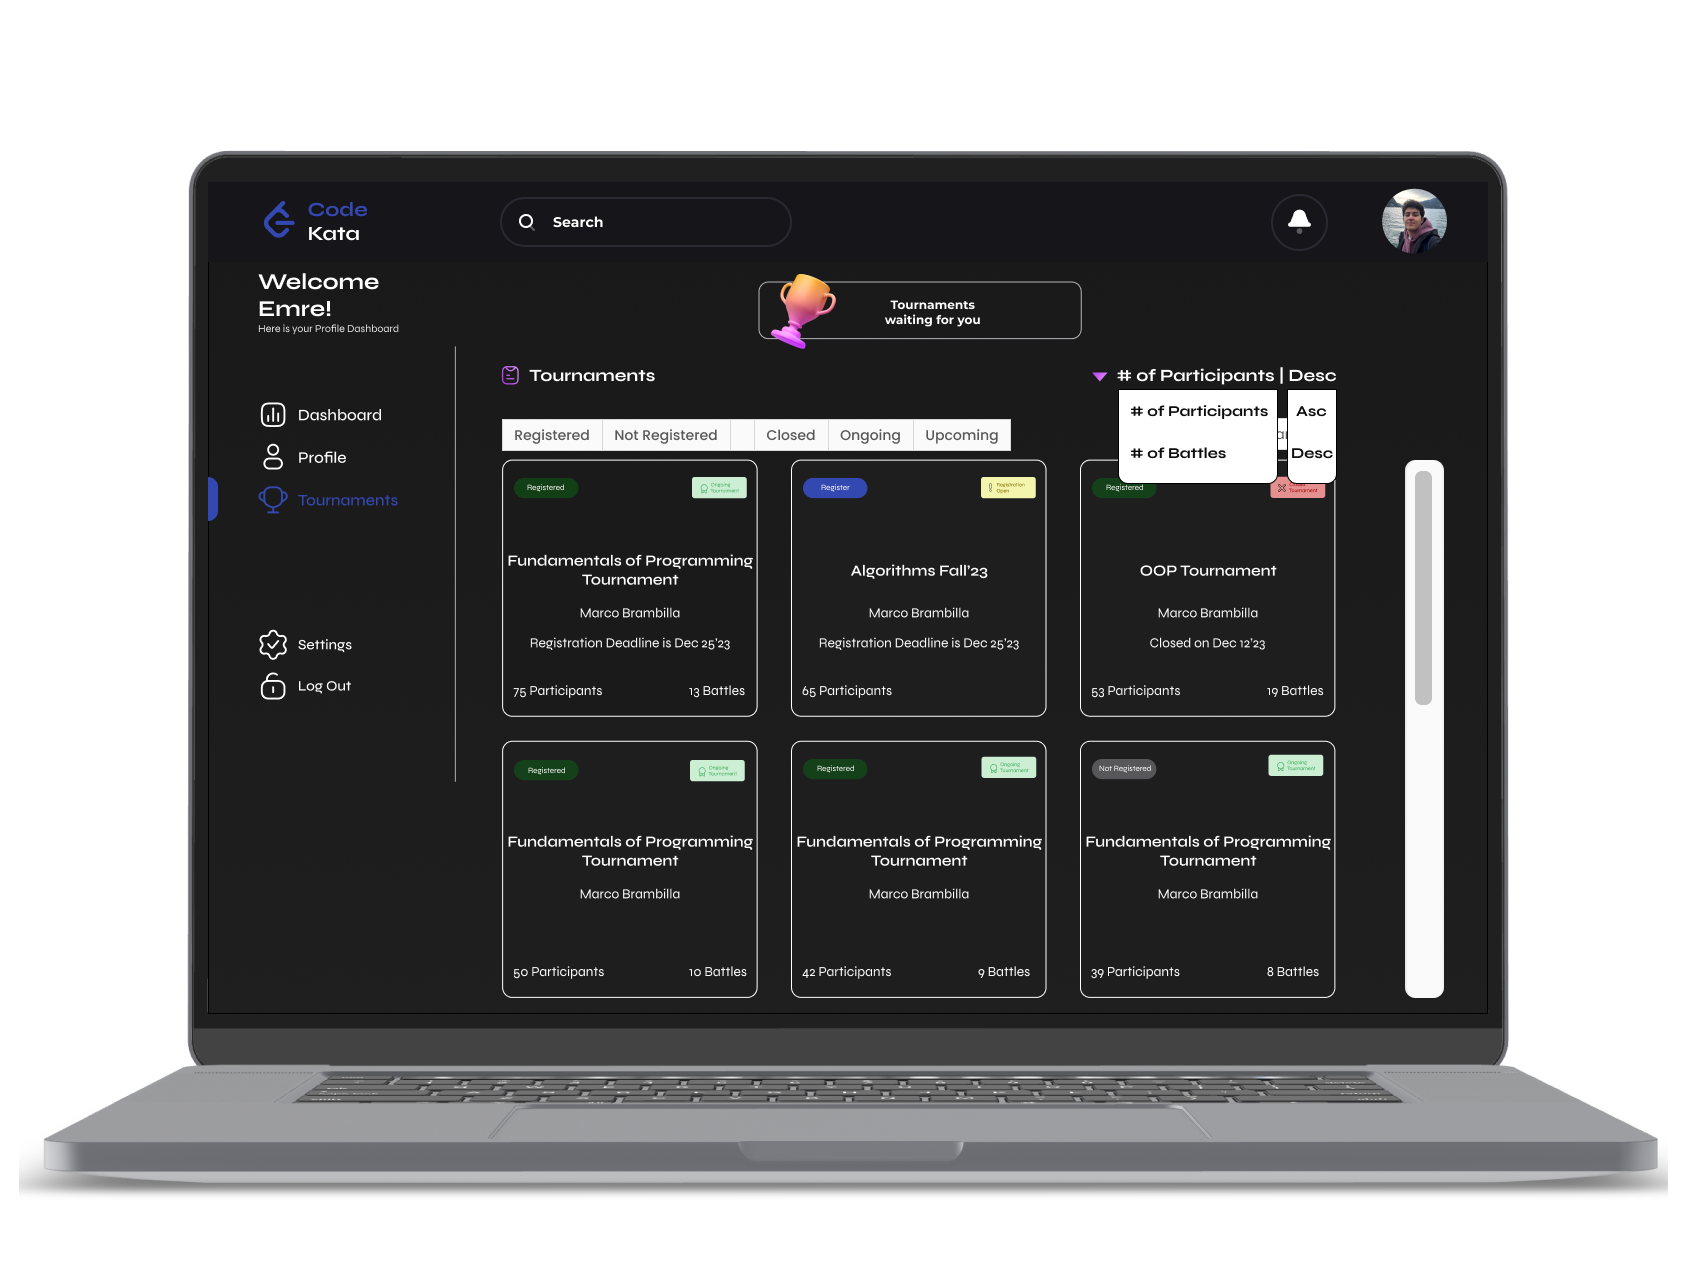
\includegraphics[scale=0.13]{Images/ui-ux/student_tournaments/student_tournaments_3.png}    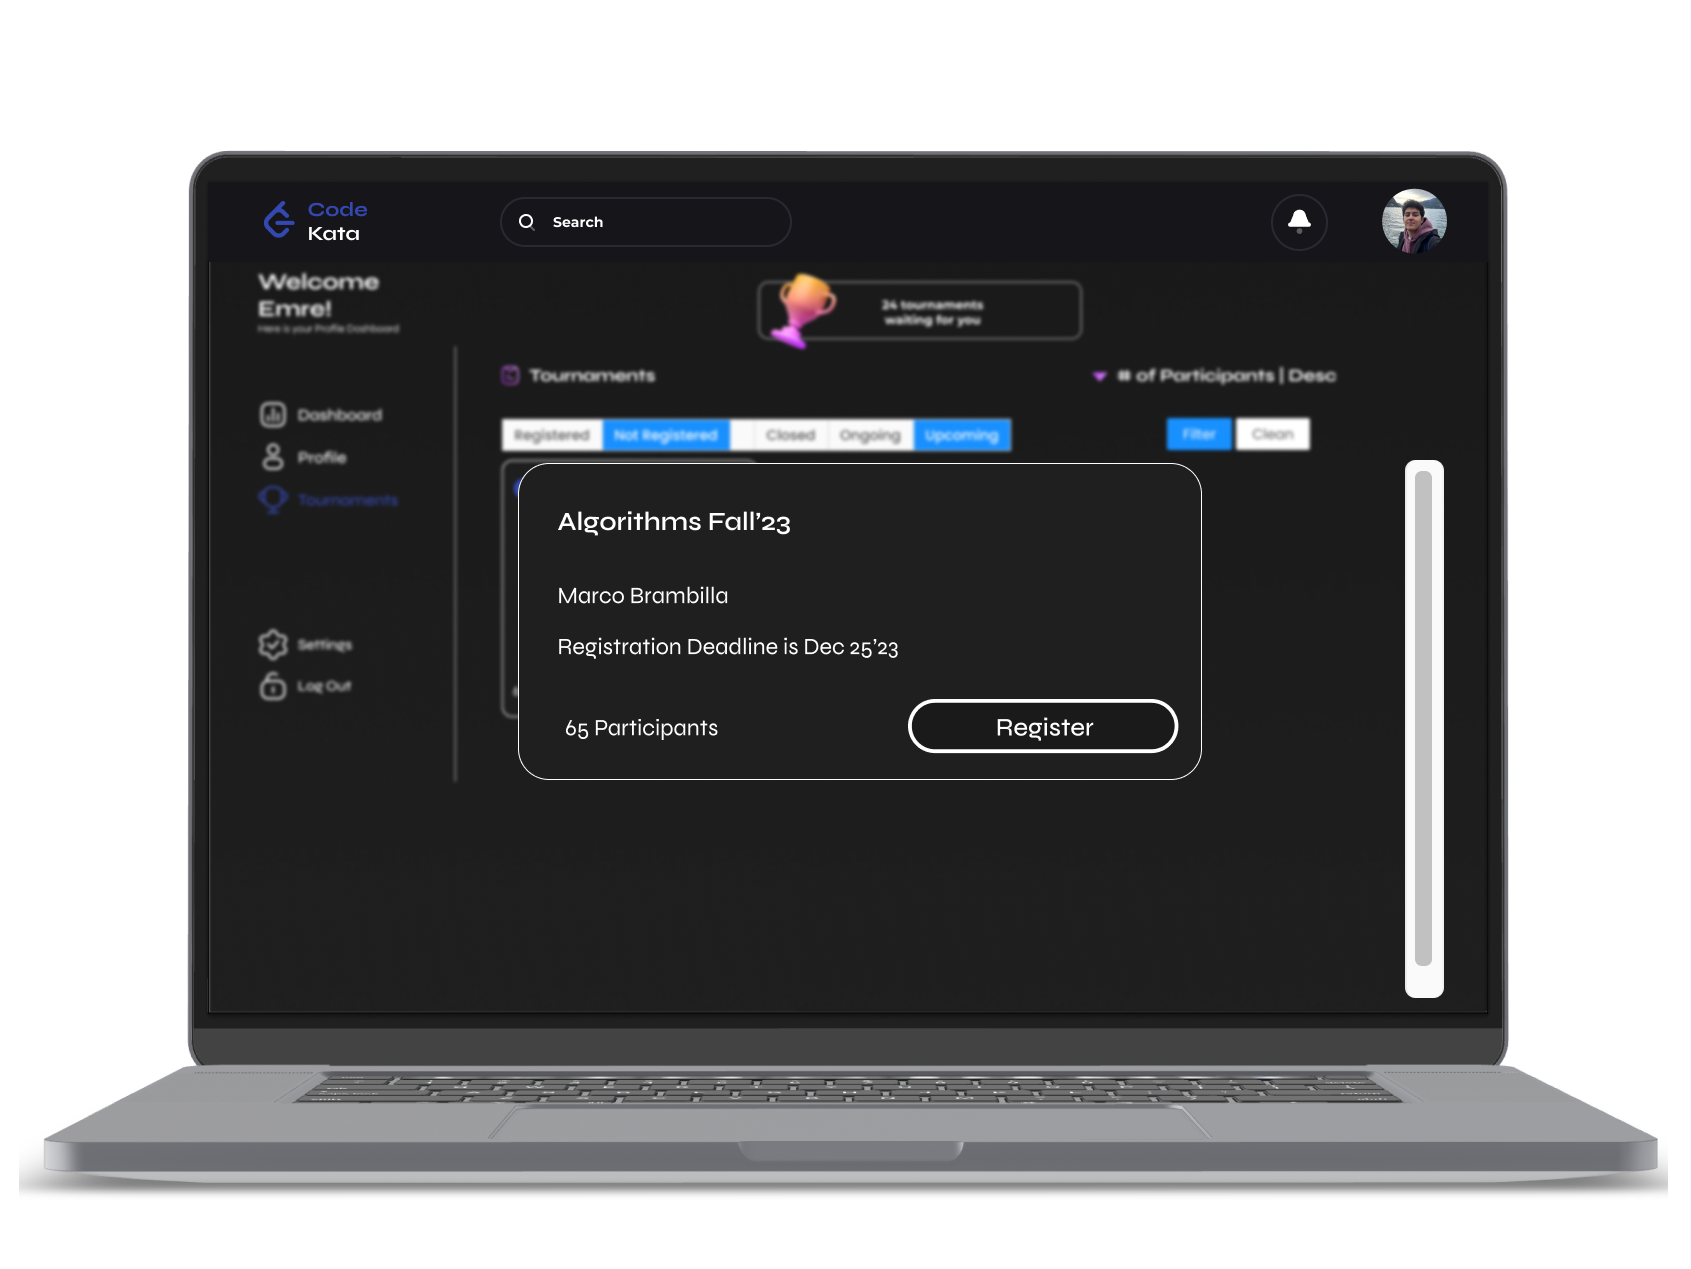
\includegraphics[scale=0.13]{Images/ui-ux/student_tournaments/student_tournaments_4.png}
        (d) Student Tournaments Page
\end{center}

\begin{center}
    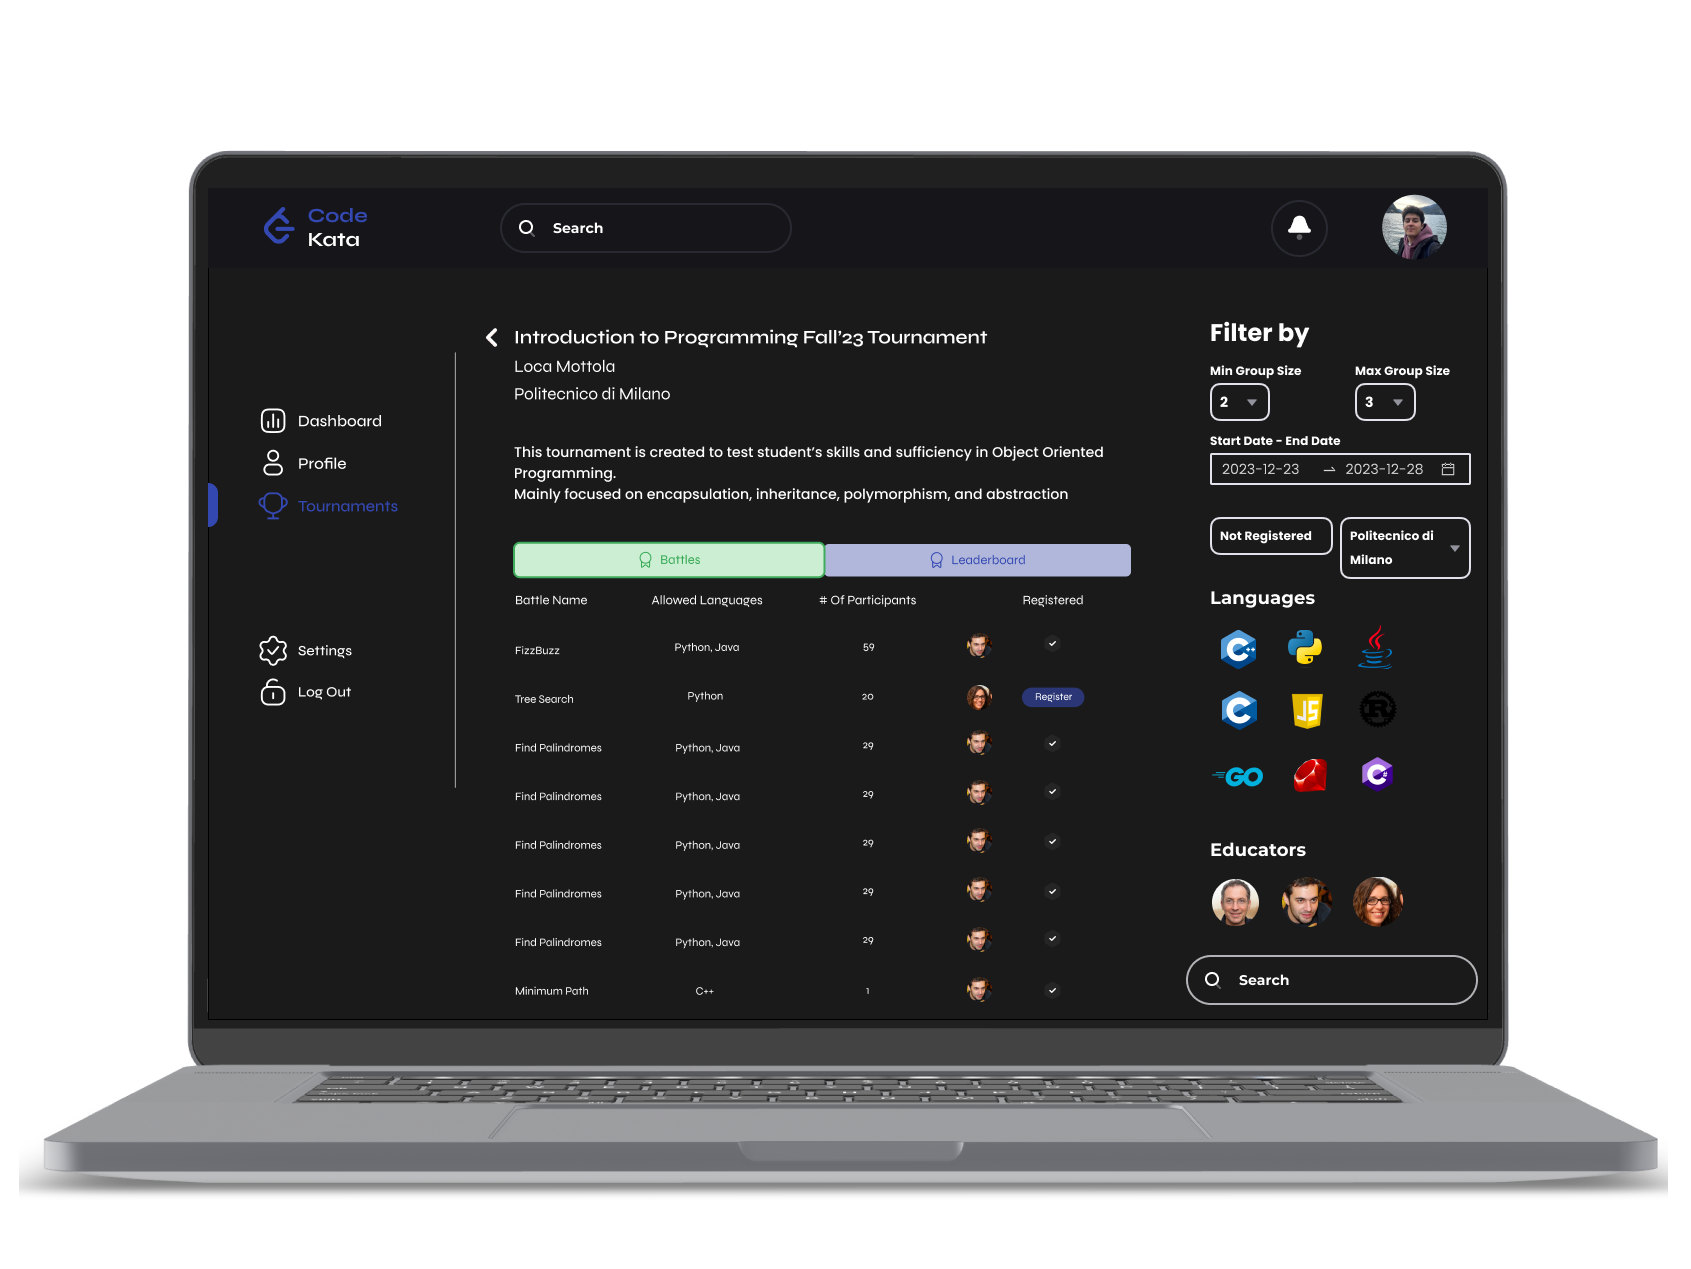
\includegraphics[scale=0.13]{Images/ui-ux/student_tournament/student_tournament_1.png}
    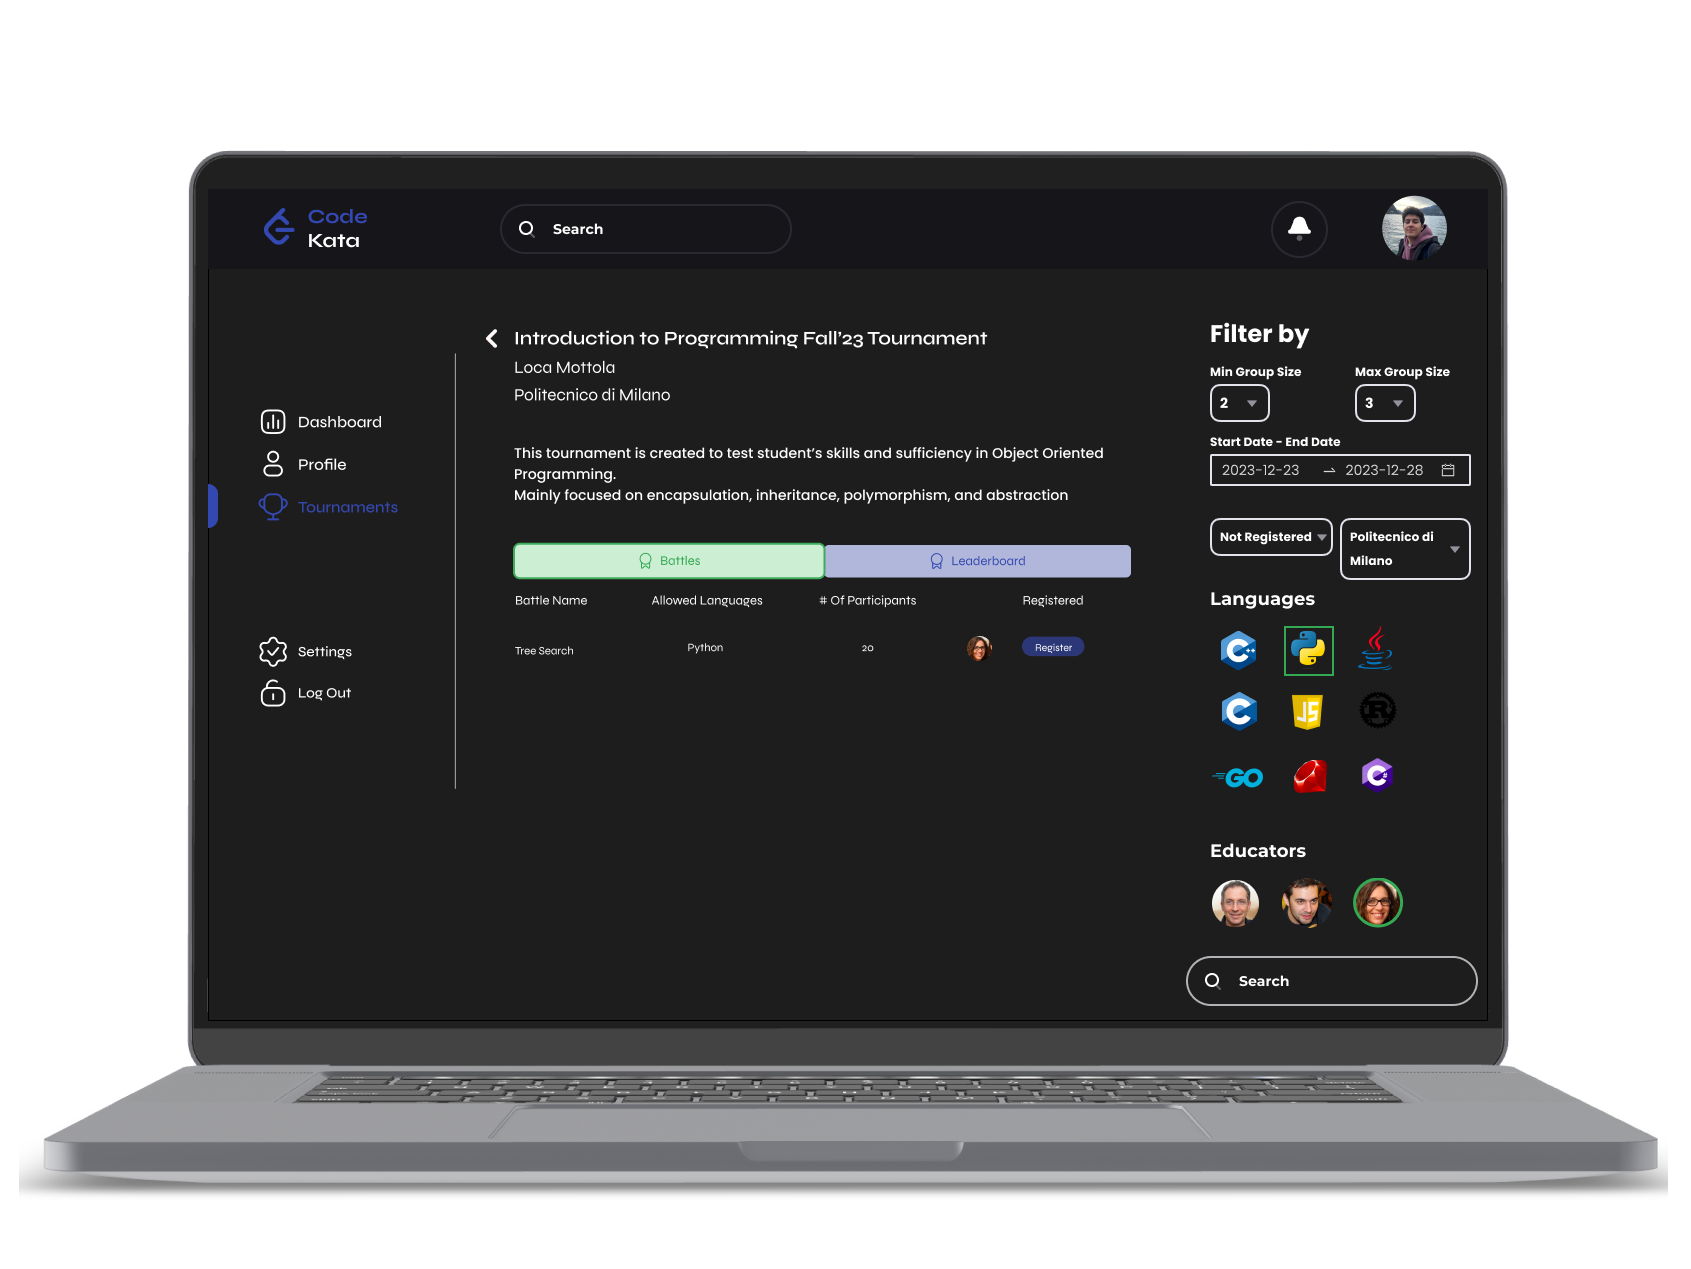
\includegraphics[scale=0.13]{Images/ui-ux/student_tournament/student_tournament_2.png}    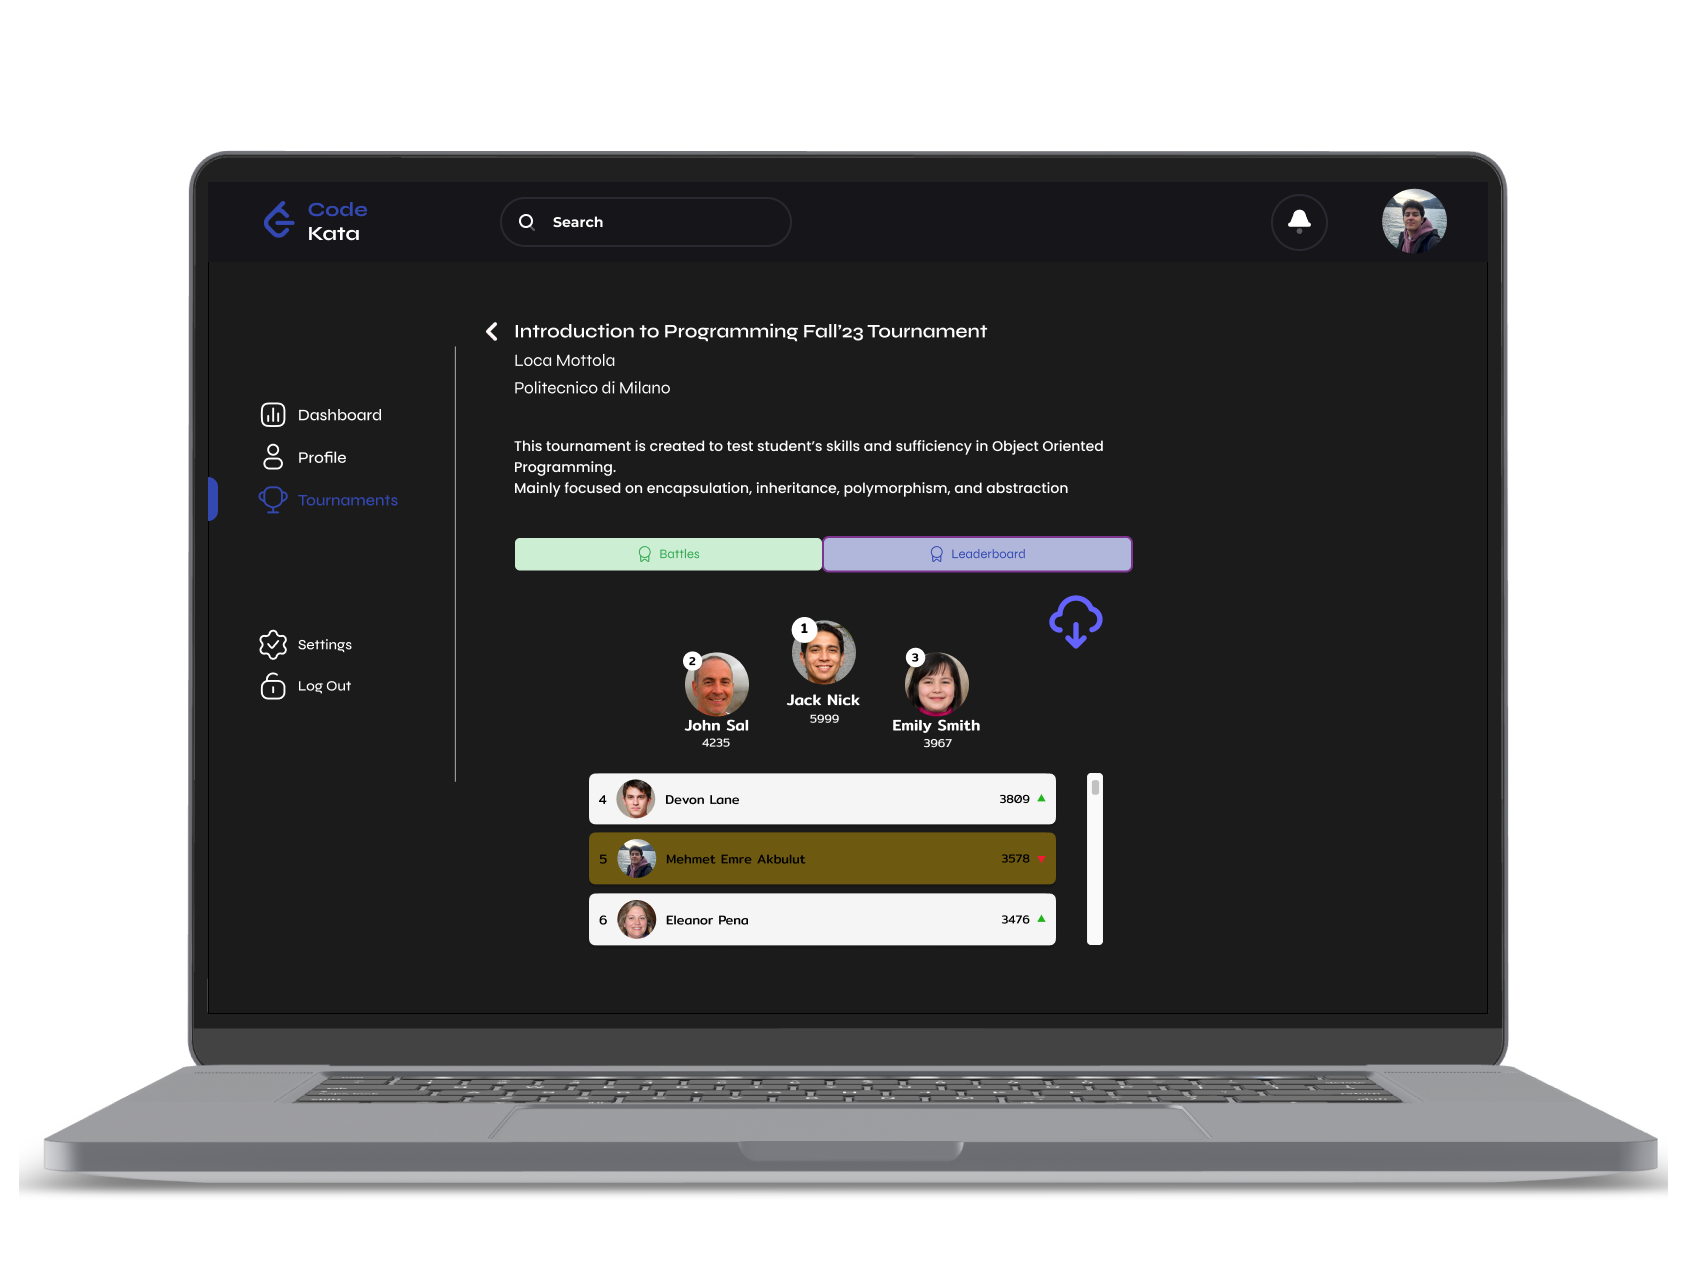
\includegraphics[scale=0.13]{Images/ui-ux/student_tournament/student_tournament_3.png} 
    \\ (e) Student visits a Tournament
\end{center}
\newpage
\begin{center}
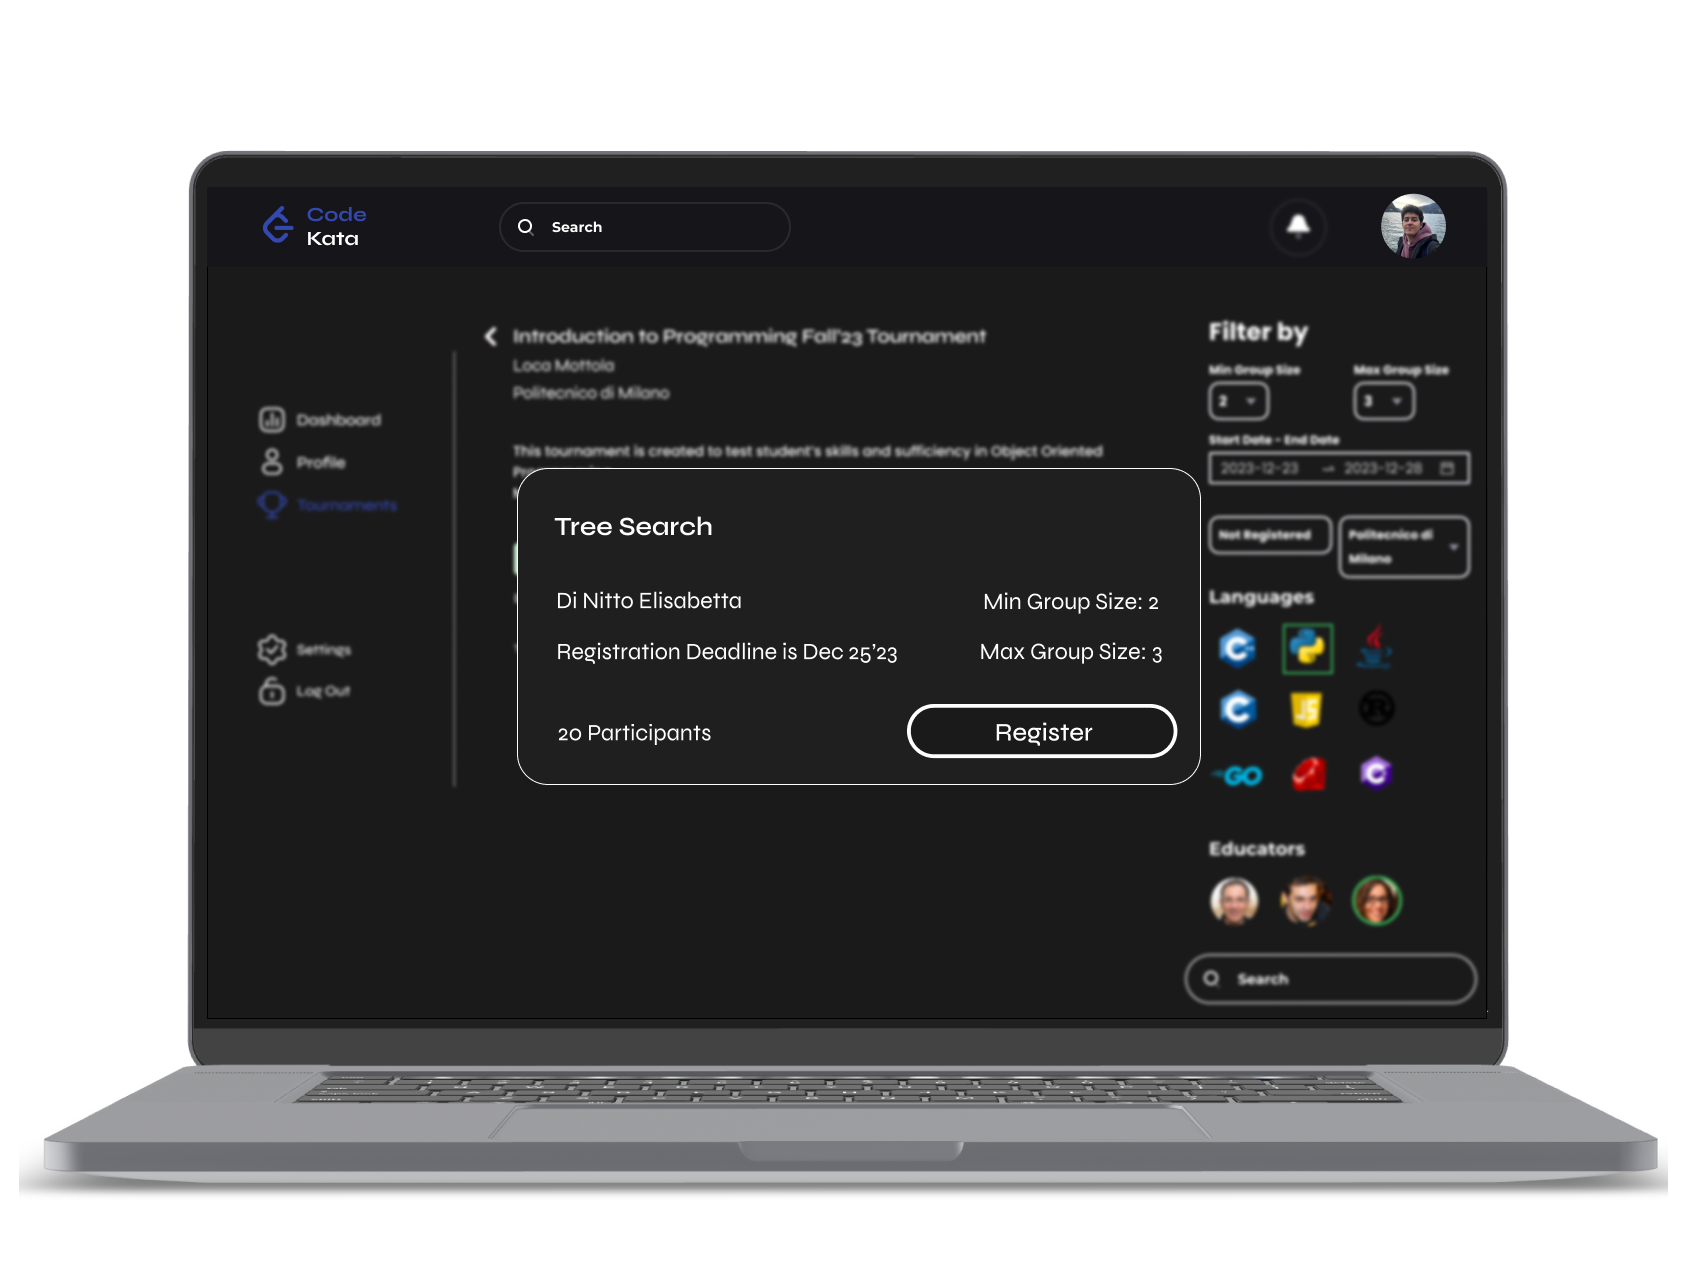
\includegraphics[scale=0.13]{Images/ui-ux/student_battle_register/student_battle_register_1.png}
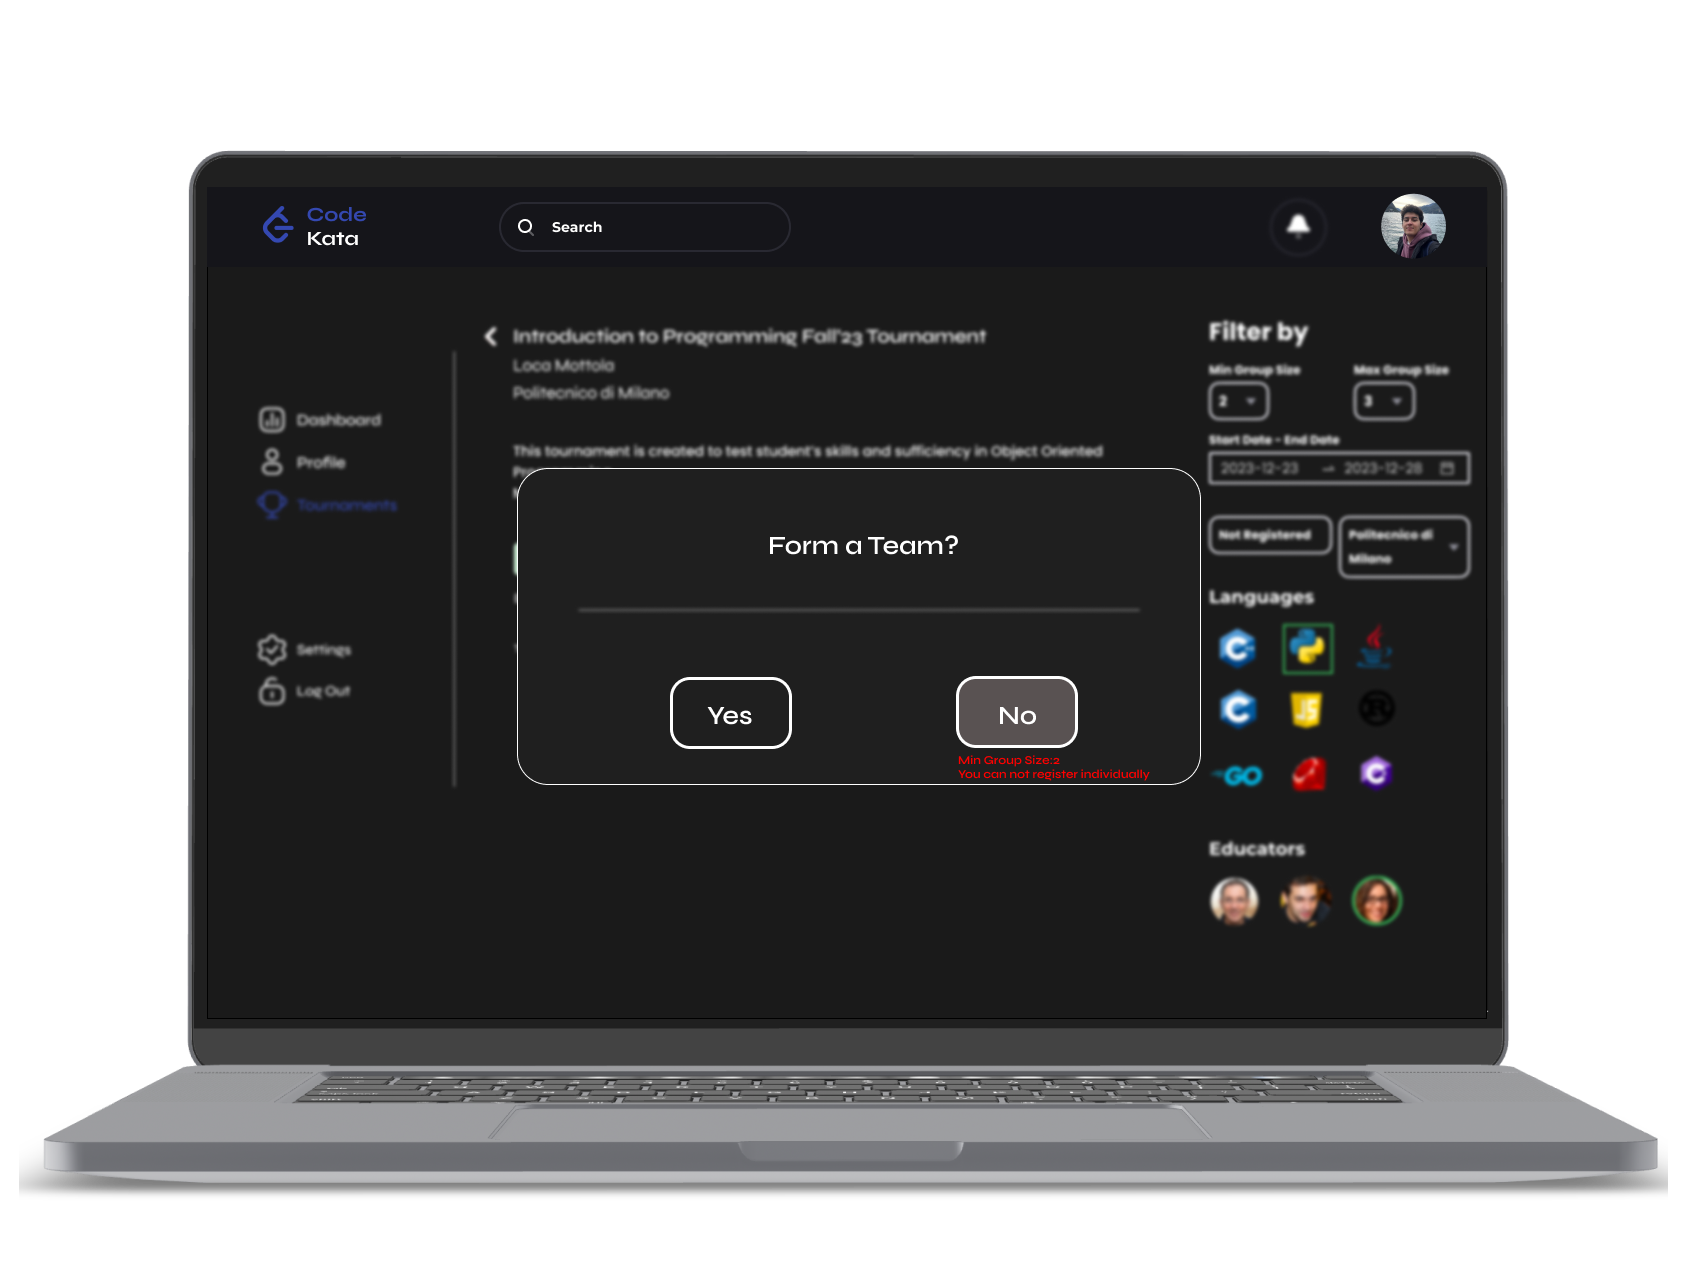
\includegraphics[scale=0.13]{Images/ui-ux/student_battle_register/student_battle_register_2.png}
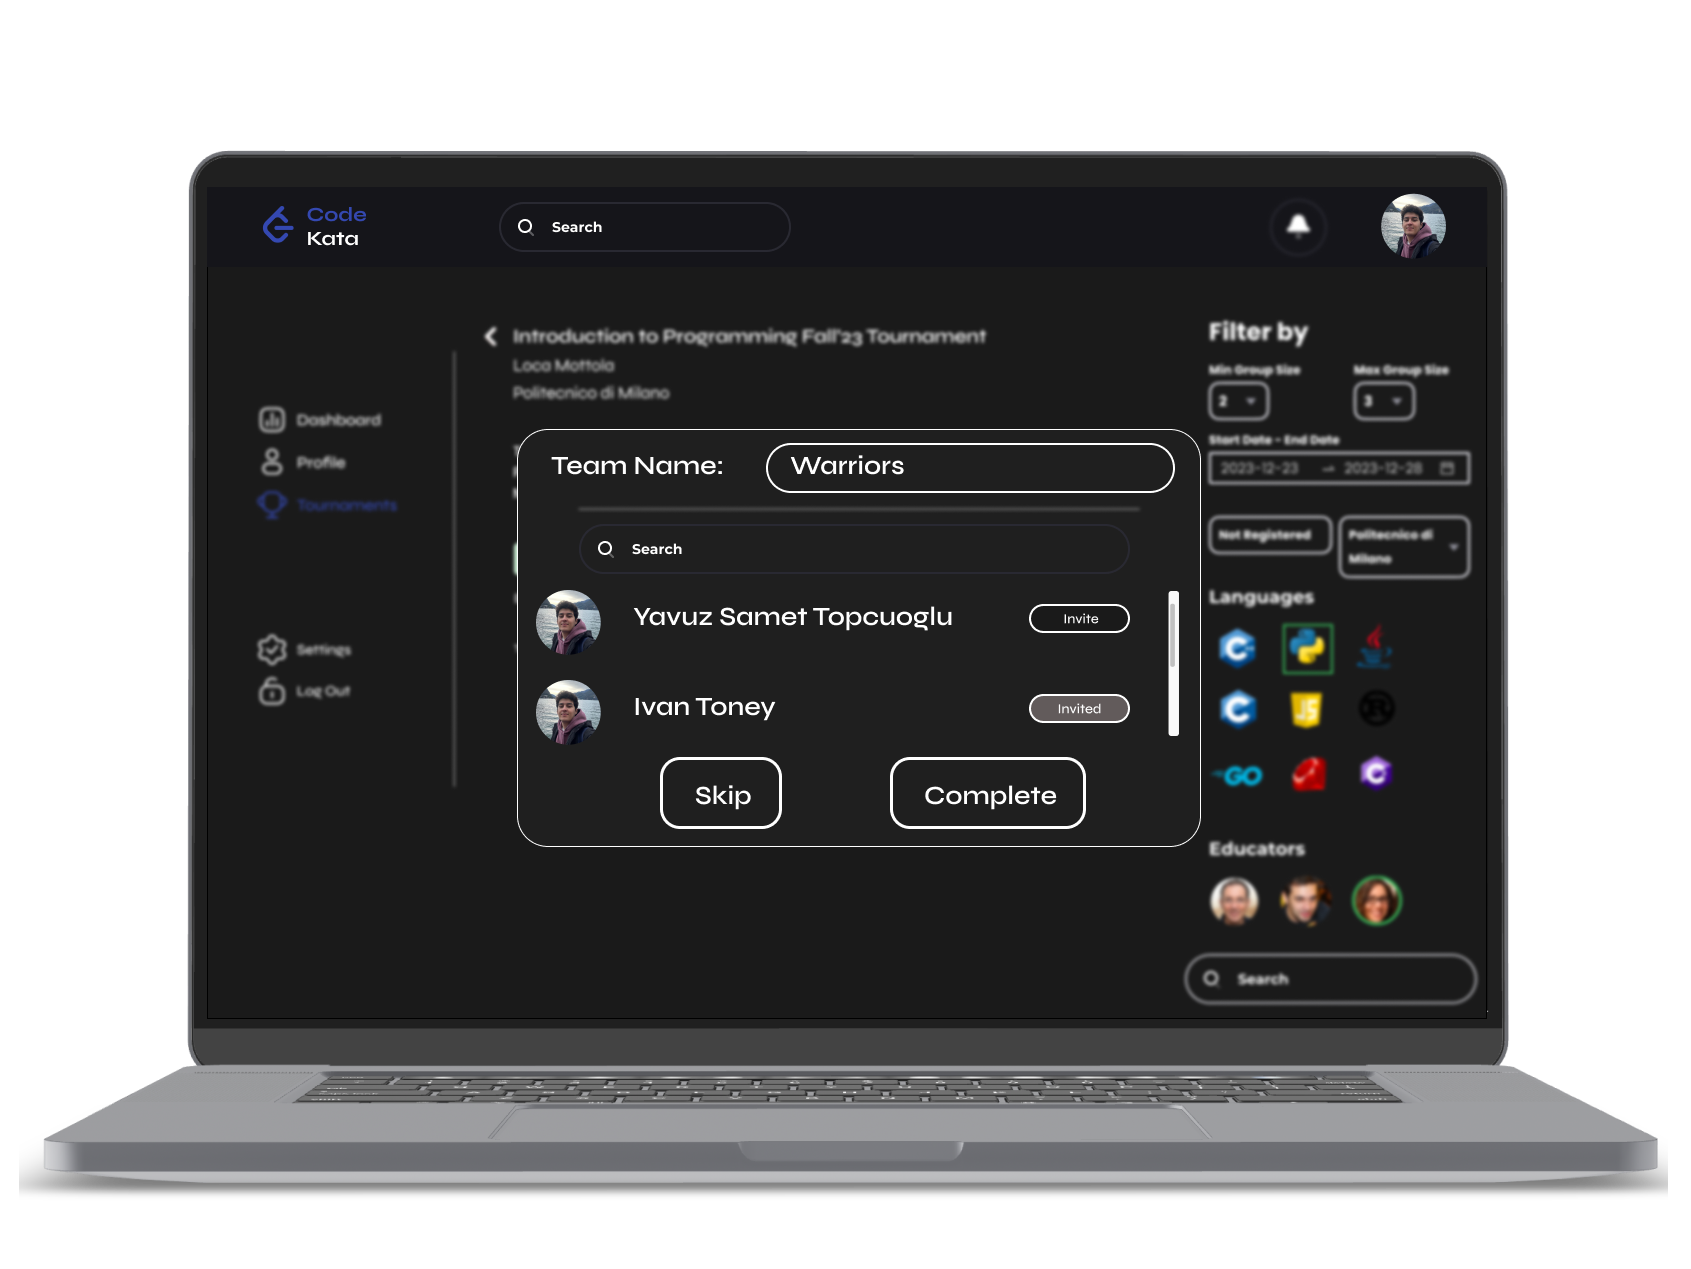
\includegraphics[scale=0.13]{Images/ui-ux/student_battle_register/student_battle_register_3.png}
\\ (f) Student Registers Battle
\end{center}
\newpage
\begin{center}
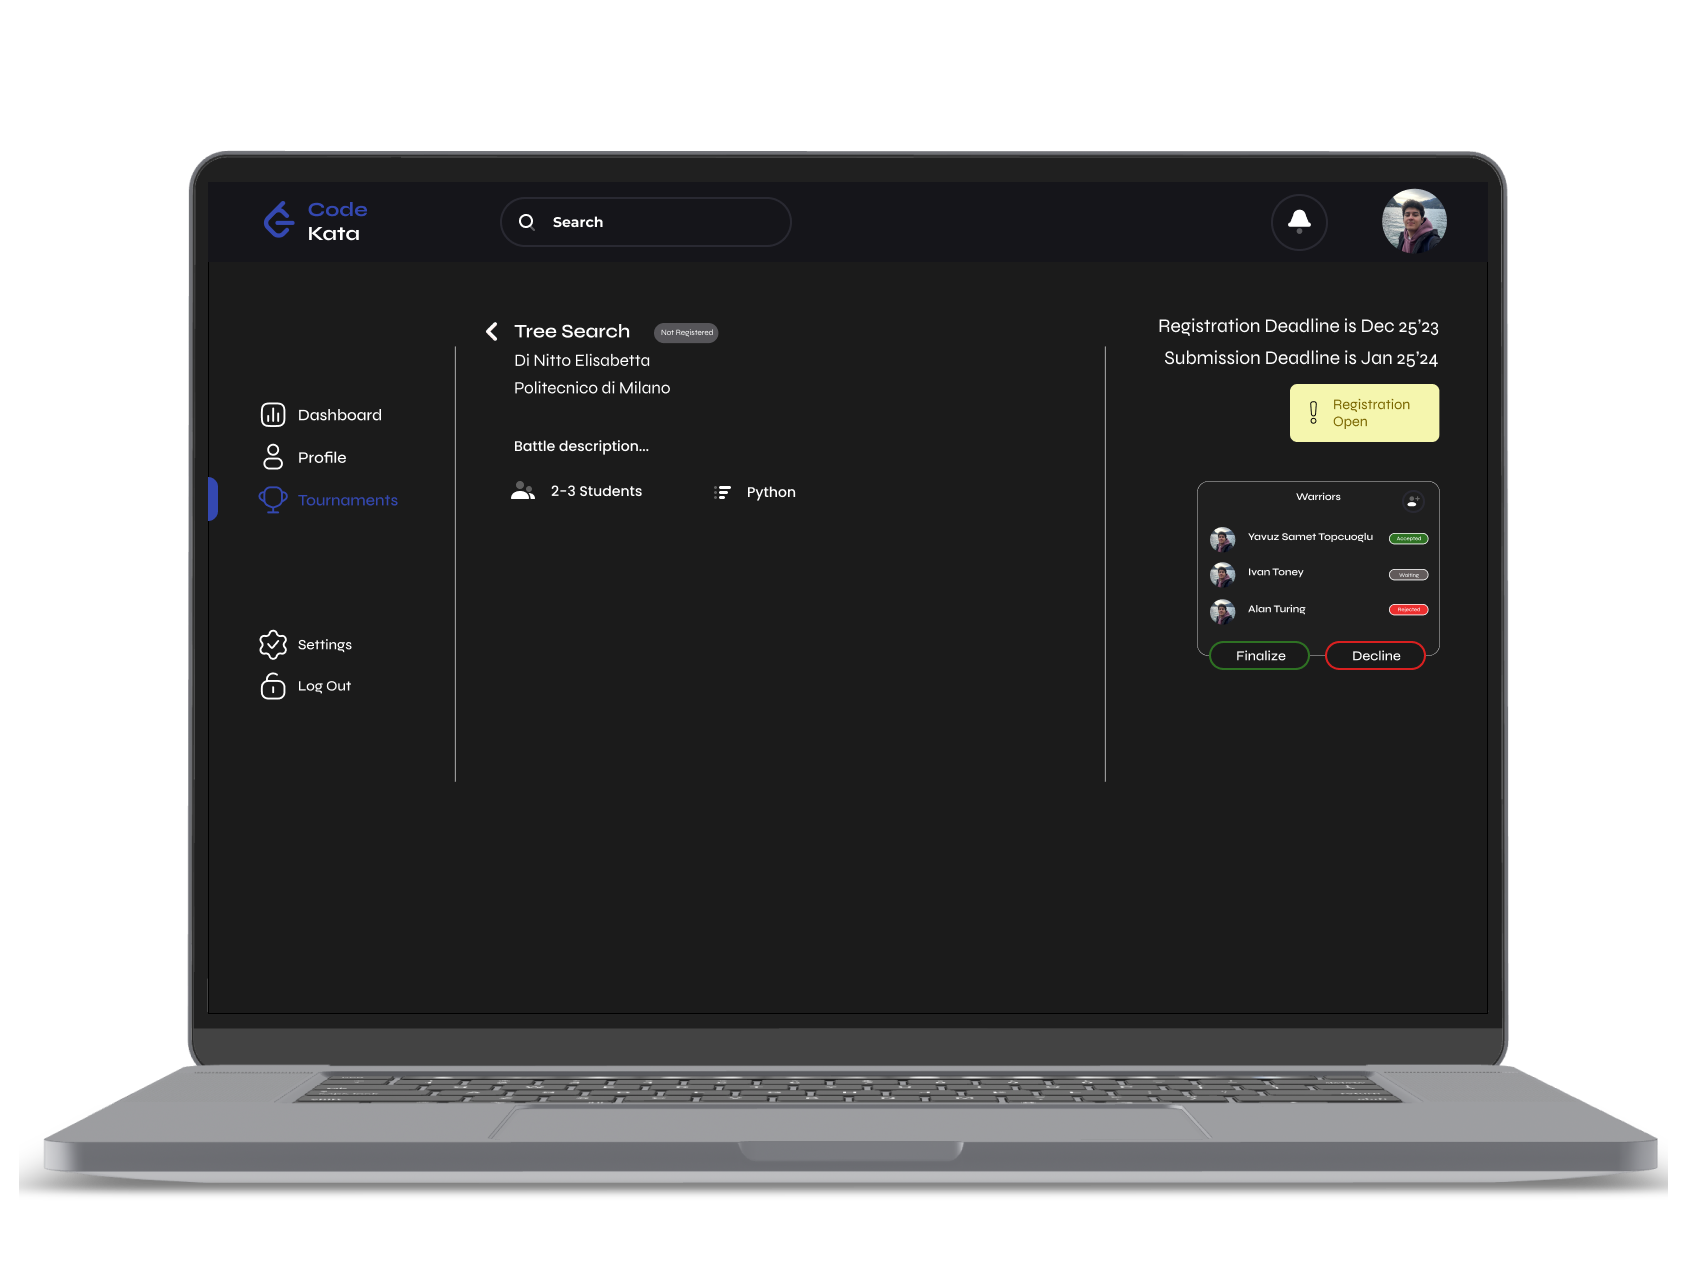
\includegraphics[scale=0.13]{Images/ui-ux/student_battle/student_battle_1.png}
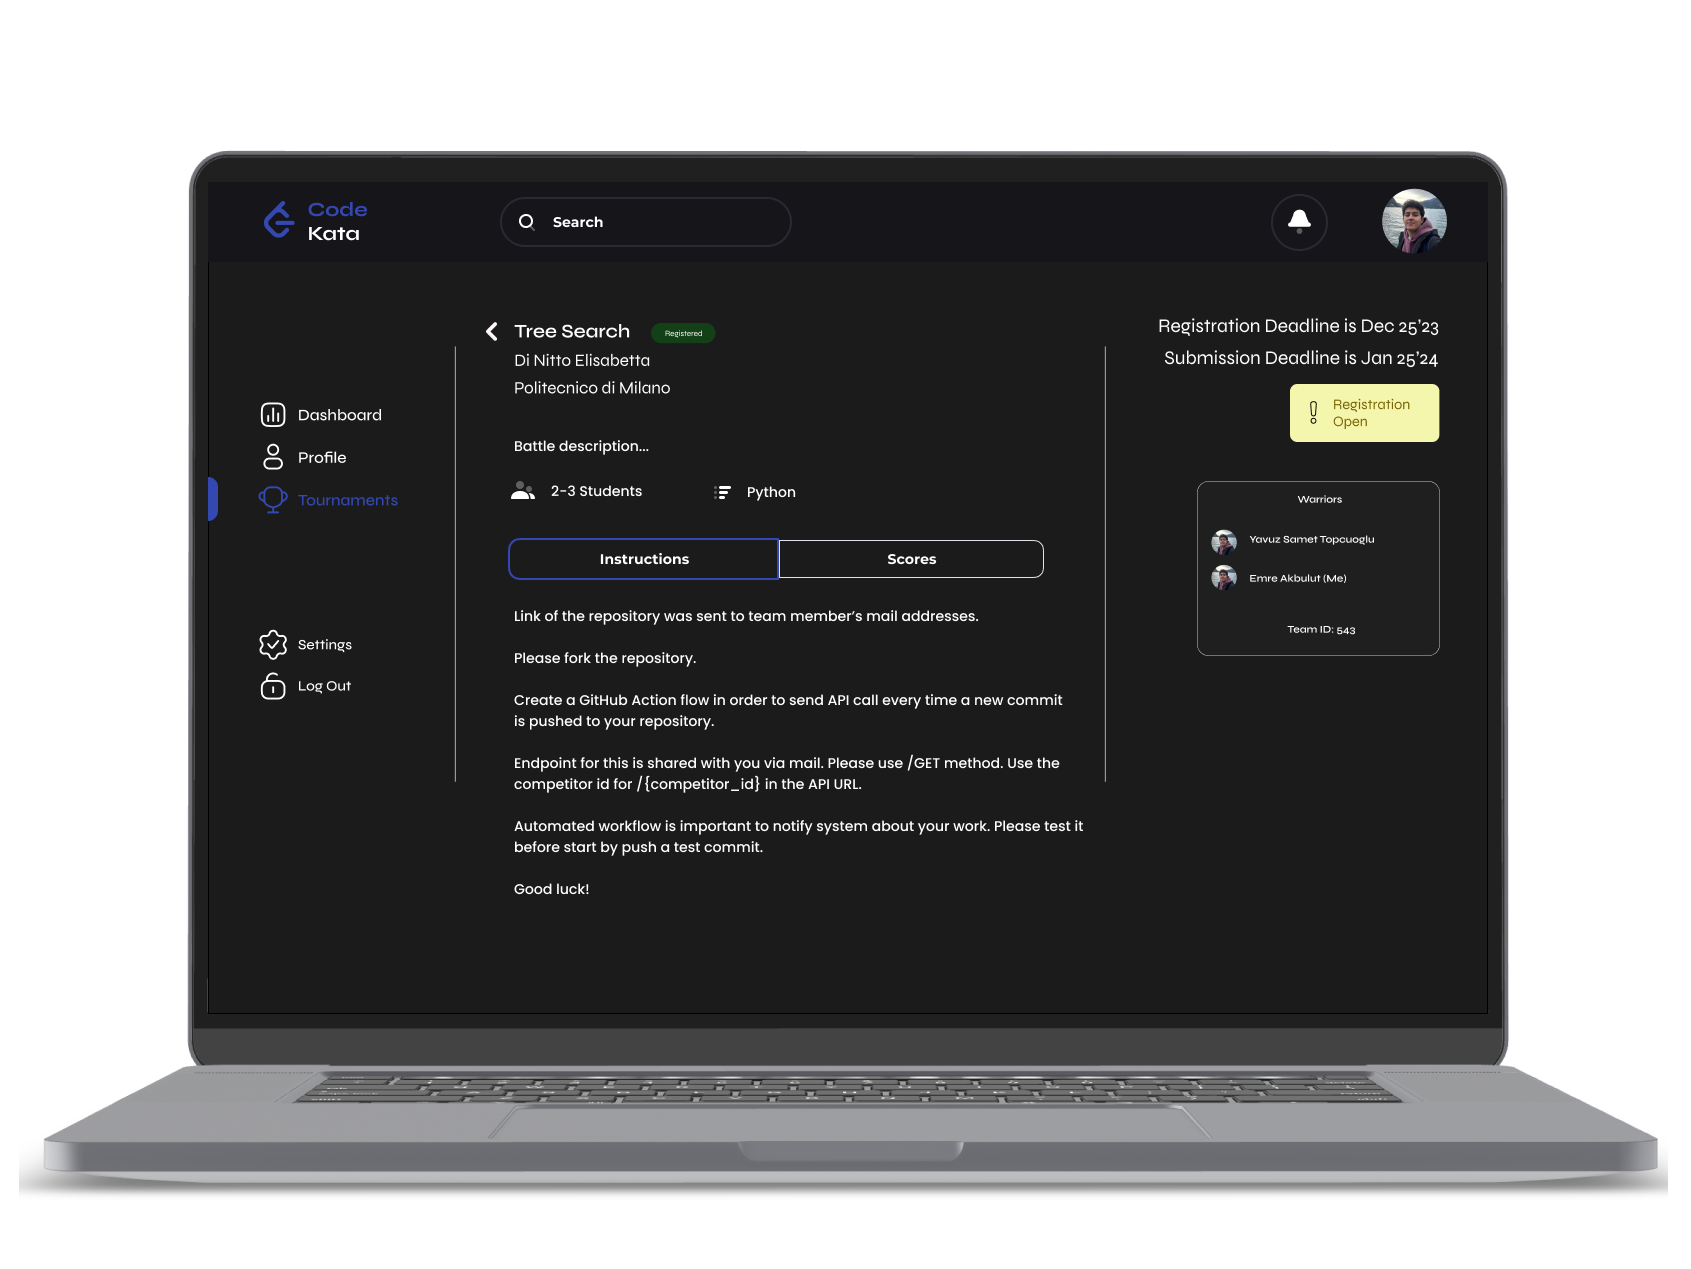
\includegraphics[scale=0.13]{Images/ui-ux/student_battle/student_battle_2.png}
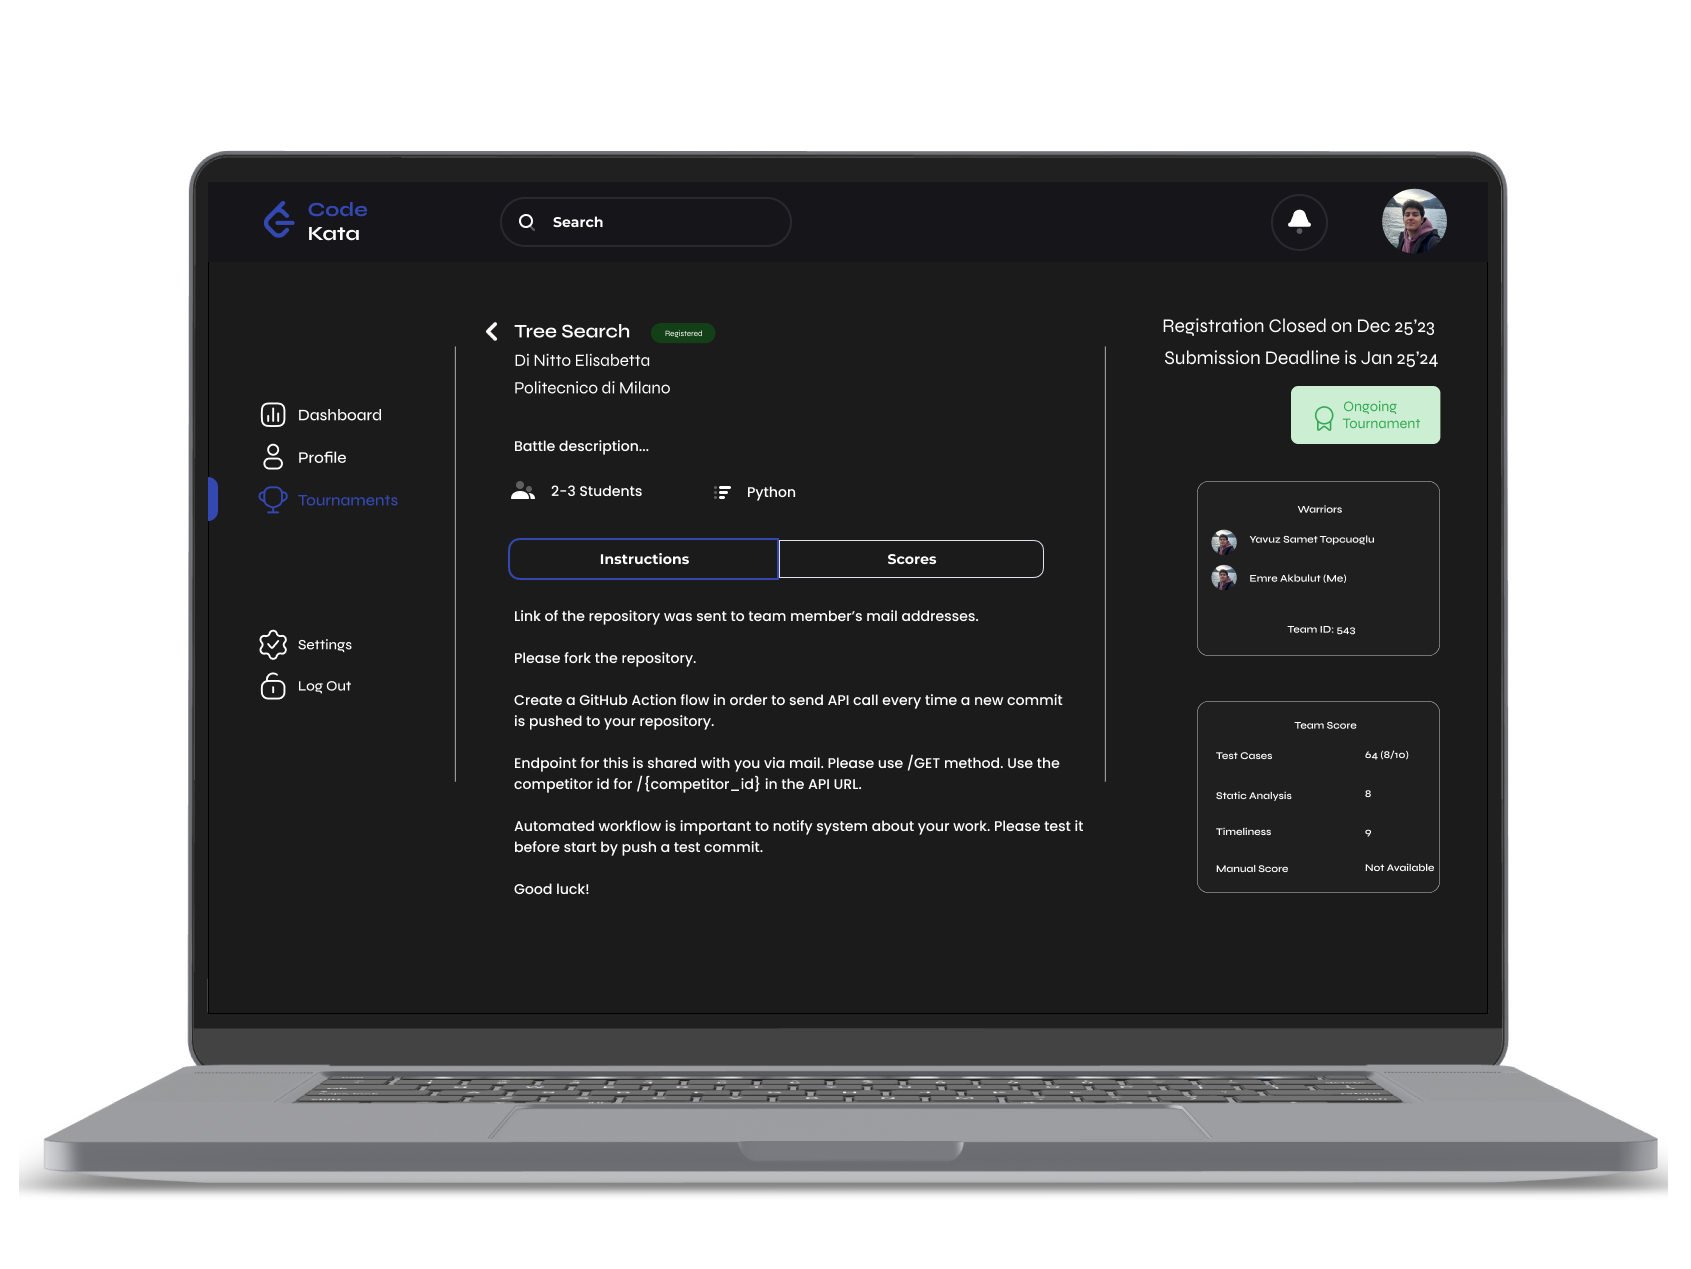
\includegraphics[scale=0.13]{Images/ui-ux/student_battle/student_battle_3.png}
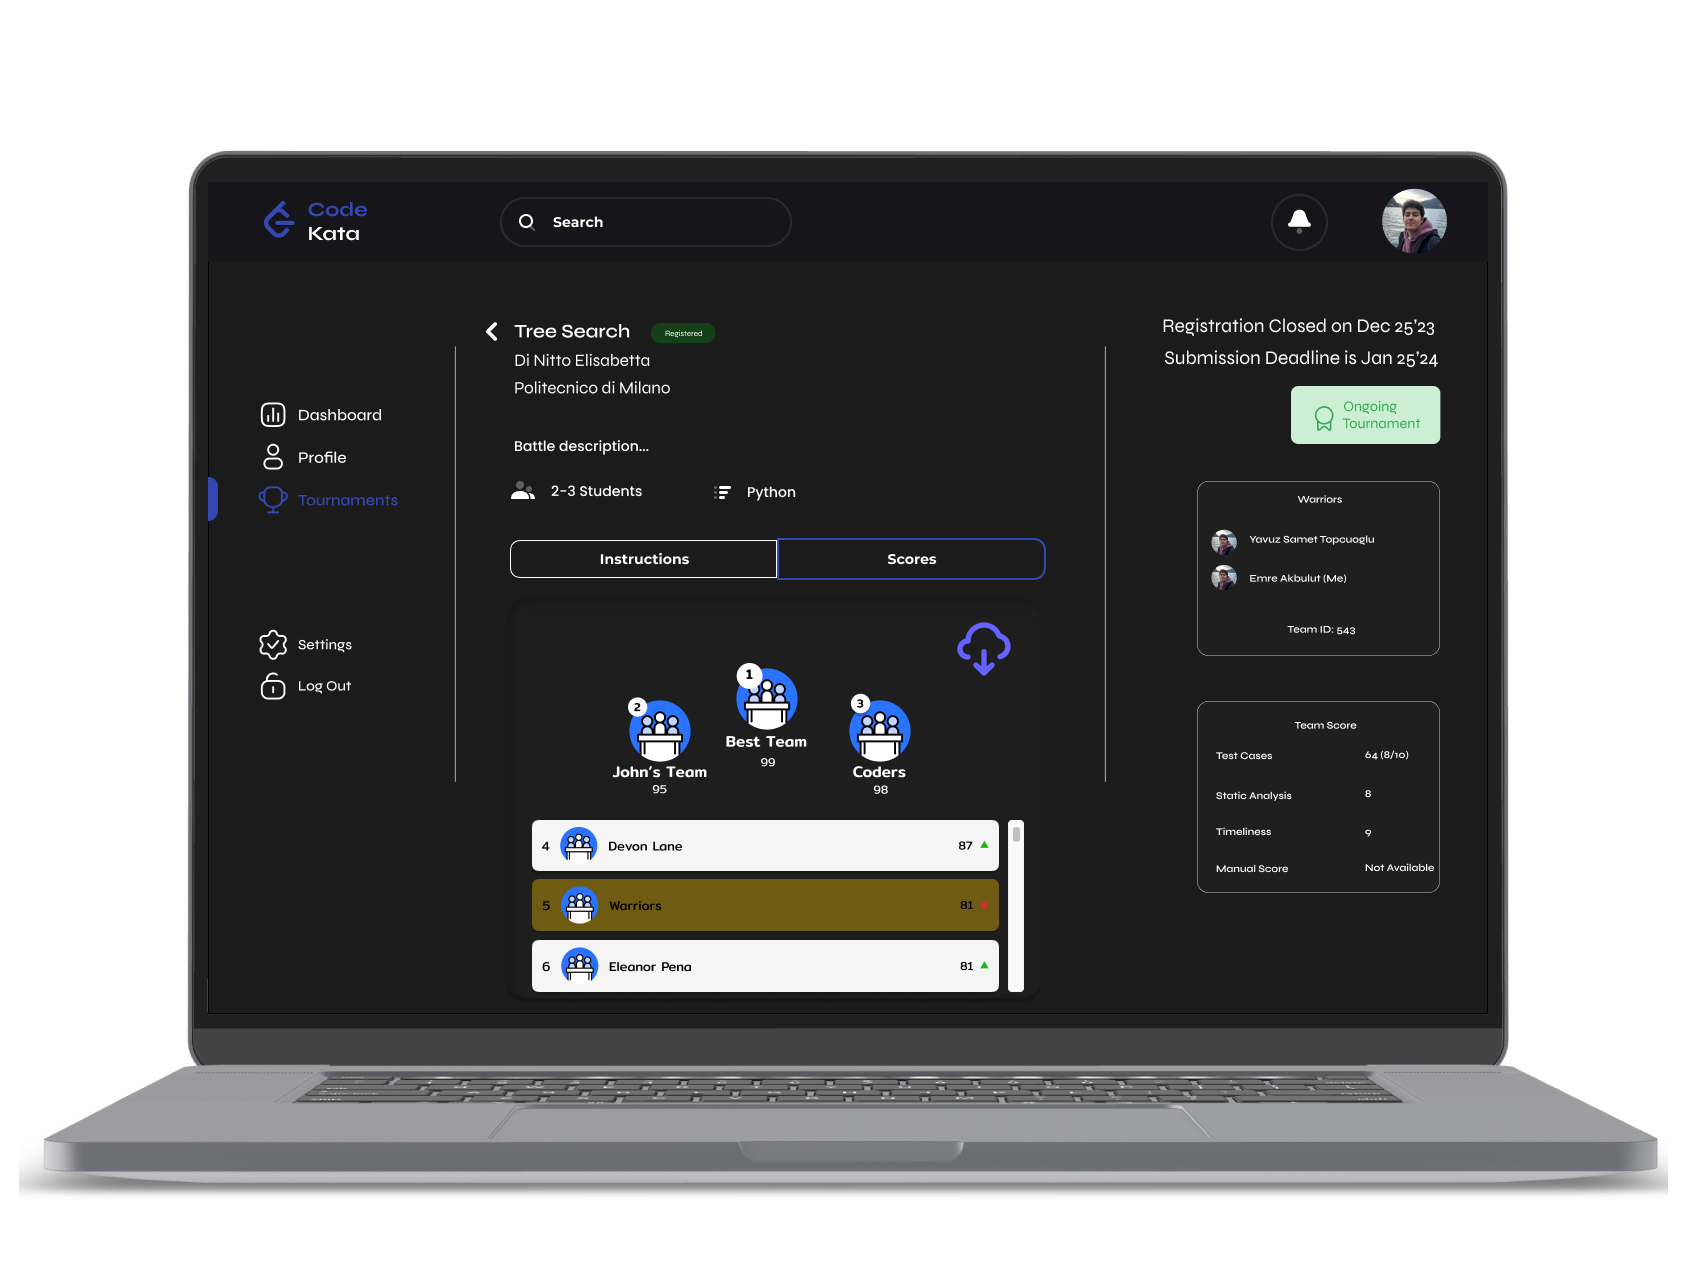
\includegraphics[scale=0.13]{Images/ui-ux/student_battle/student_battle_4.png}
      (g) Battle Screen for Student
\end{center}

\begin{center}
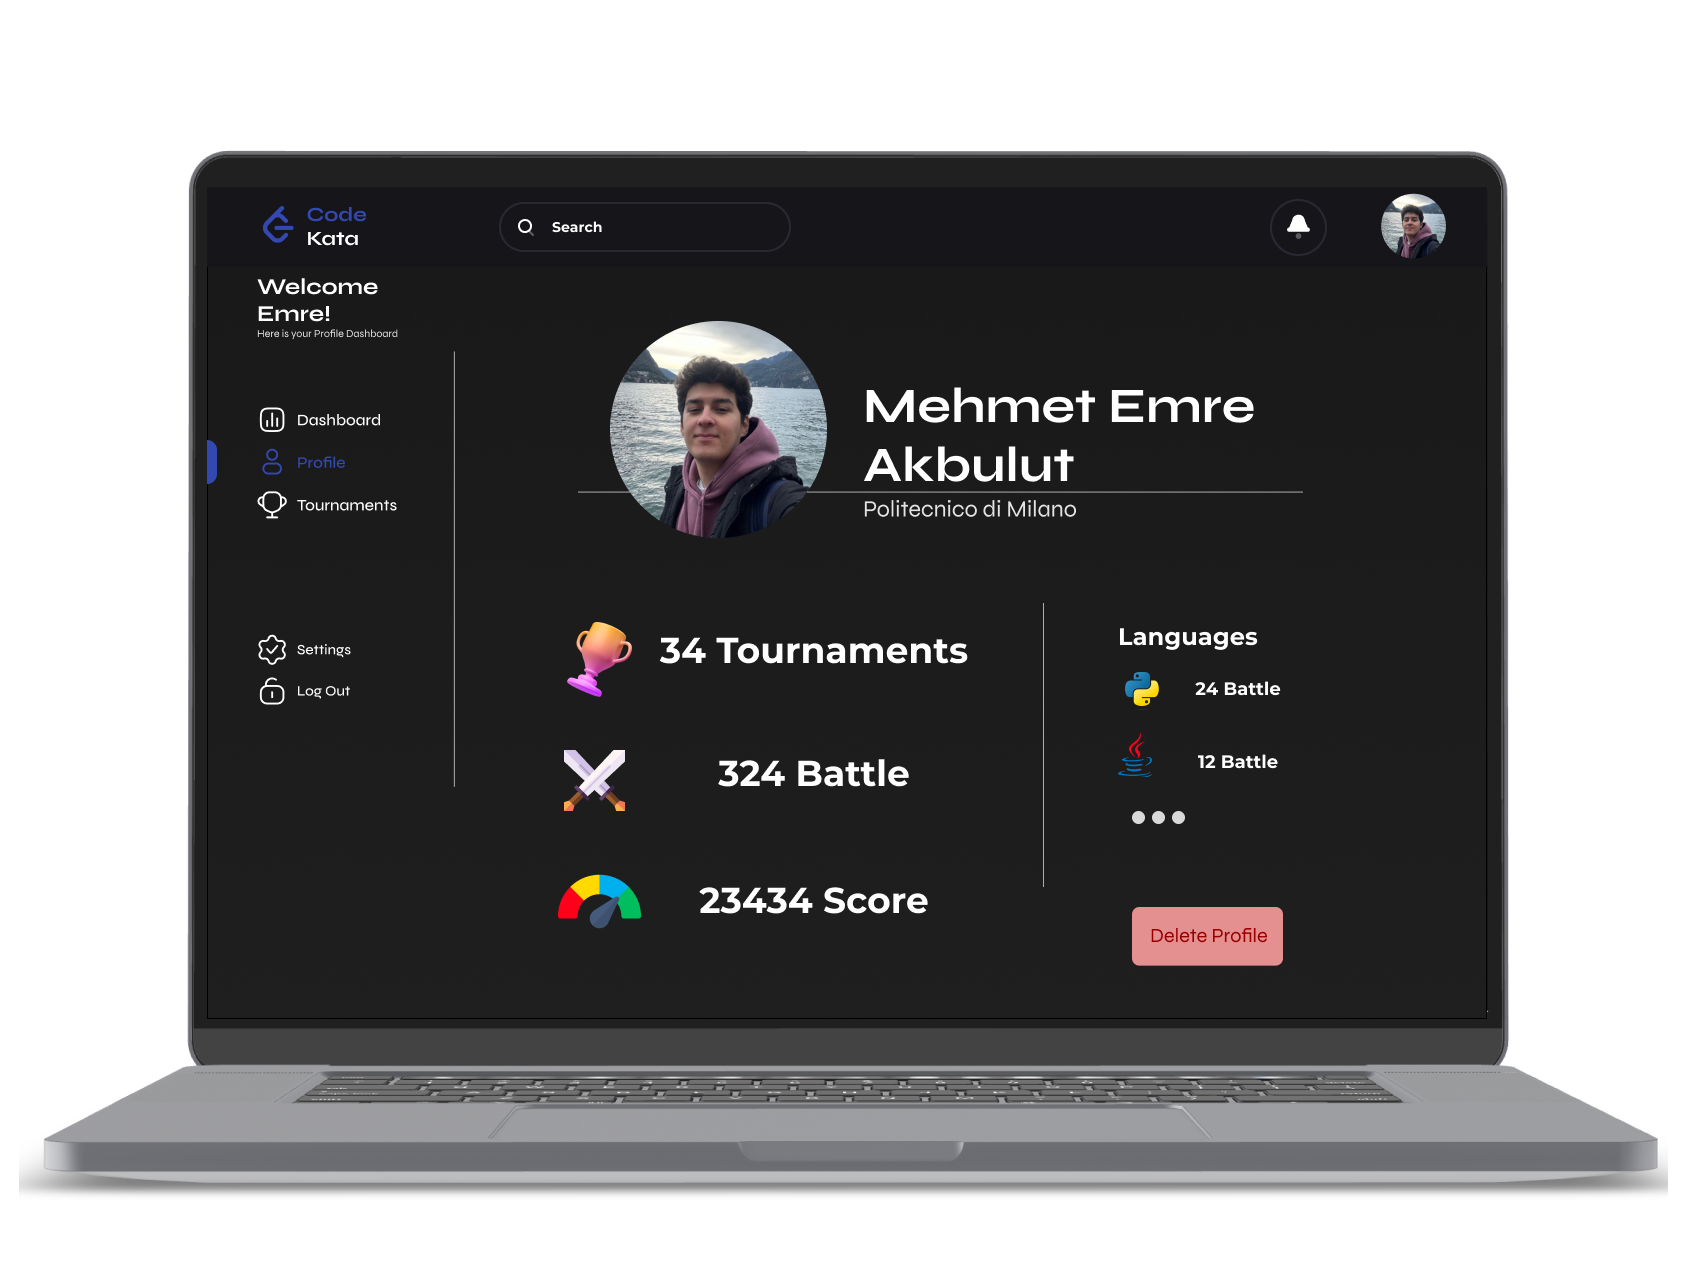
\includegraphics[scale=0.13]{Images/ui-ux/student_profile_settings/student_profile.png}
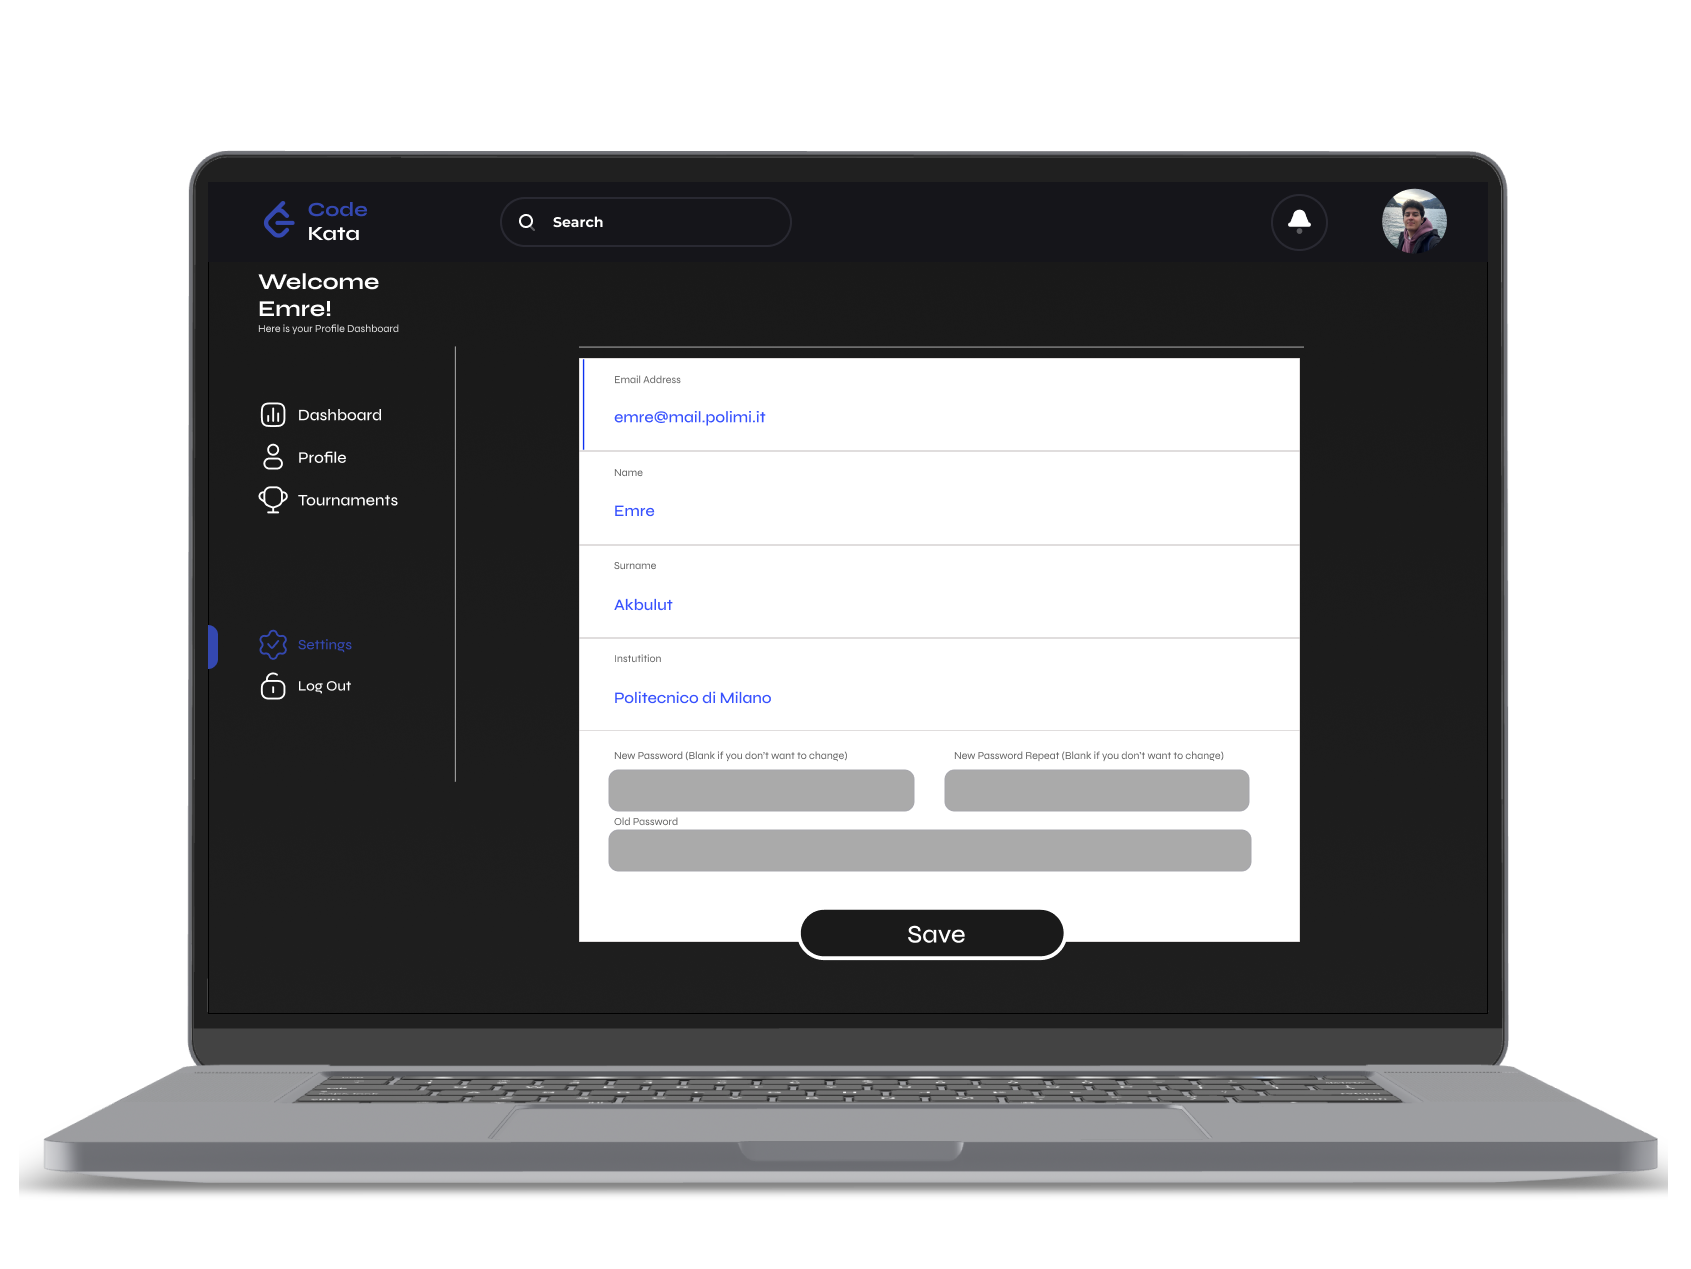
\includegraphics[scale=0.13]{Images/ui-ux/student_profile_settings/student_settings.png}
        (h) Profile and Settings for Student
\end{center}
\newpage
\begin{center}
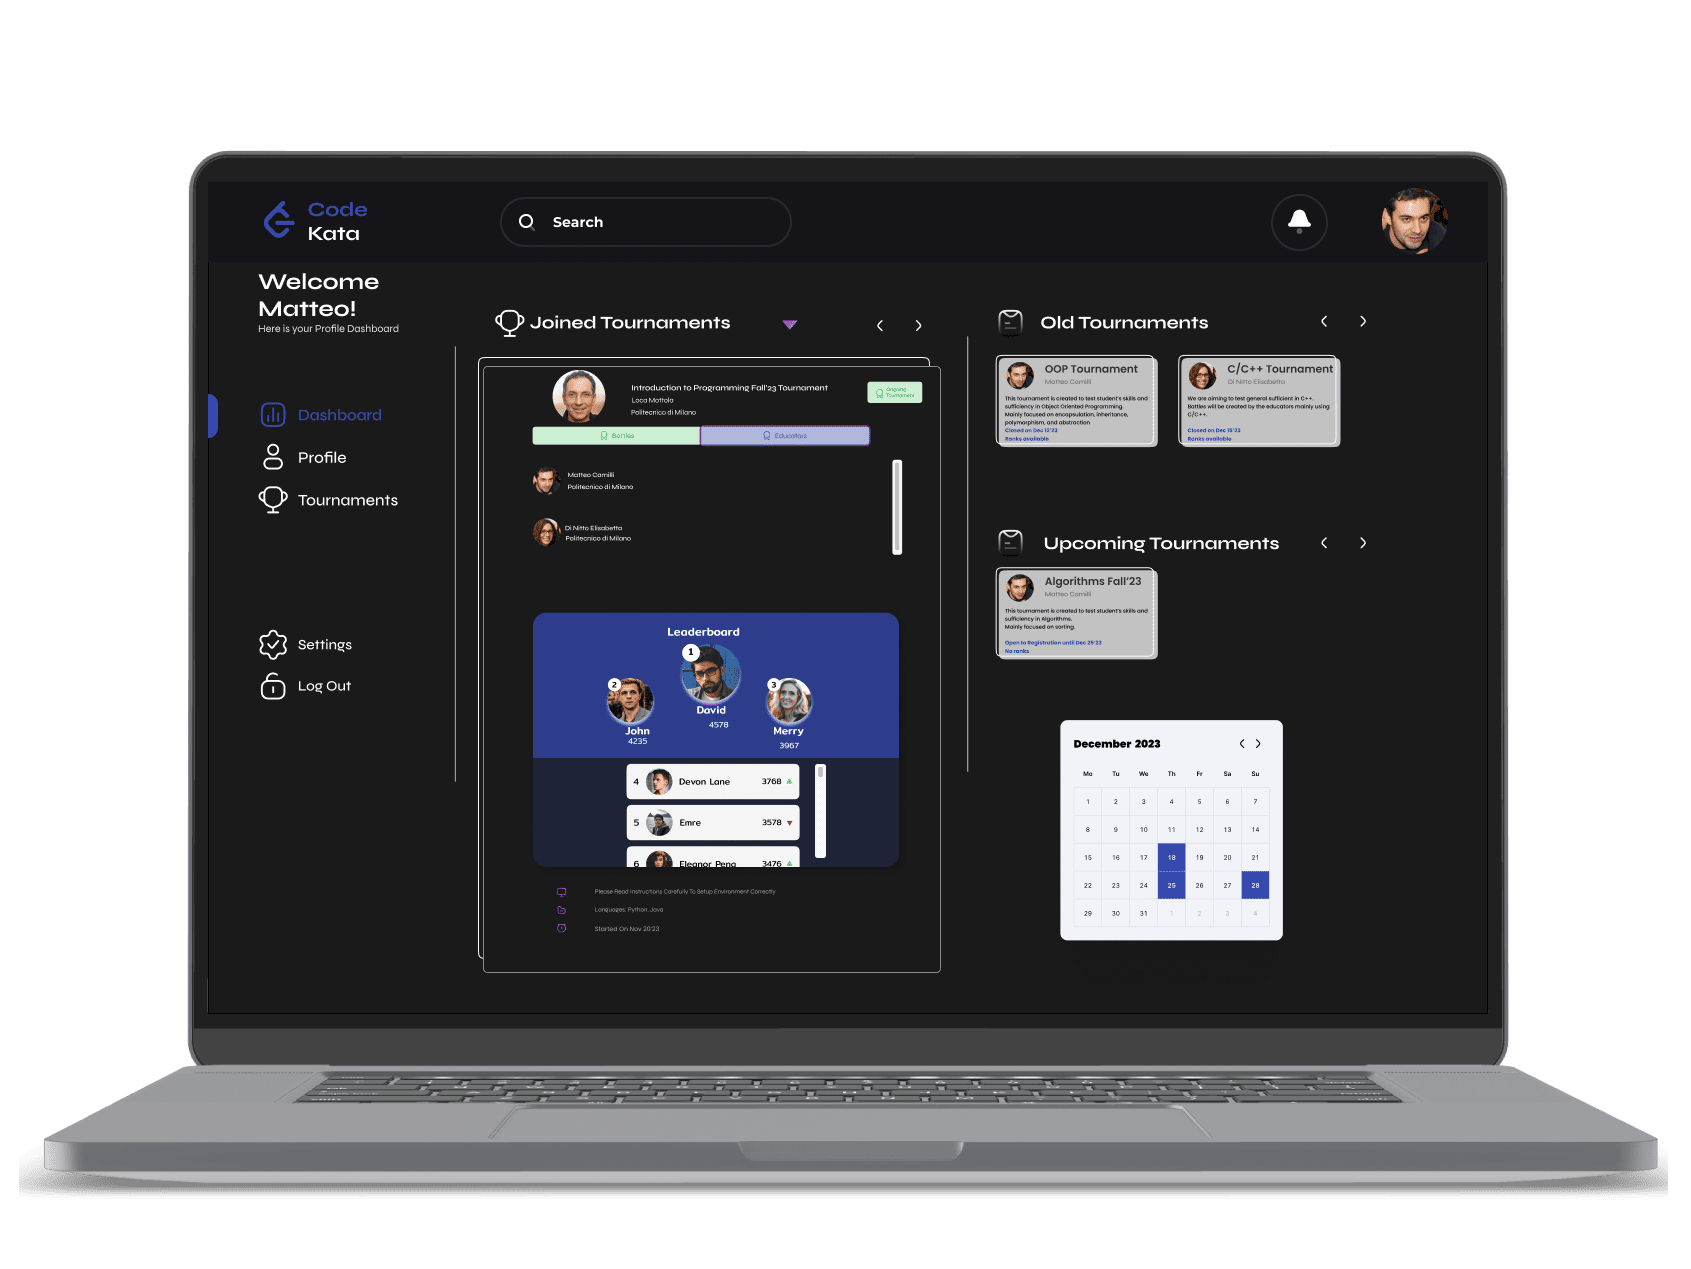
\includegraphics[scale=0.13]{Images/ui-ux/educator_dashboard/educator_dashboard_1.png}
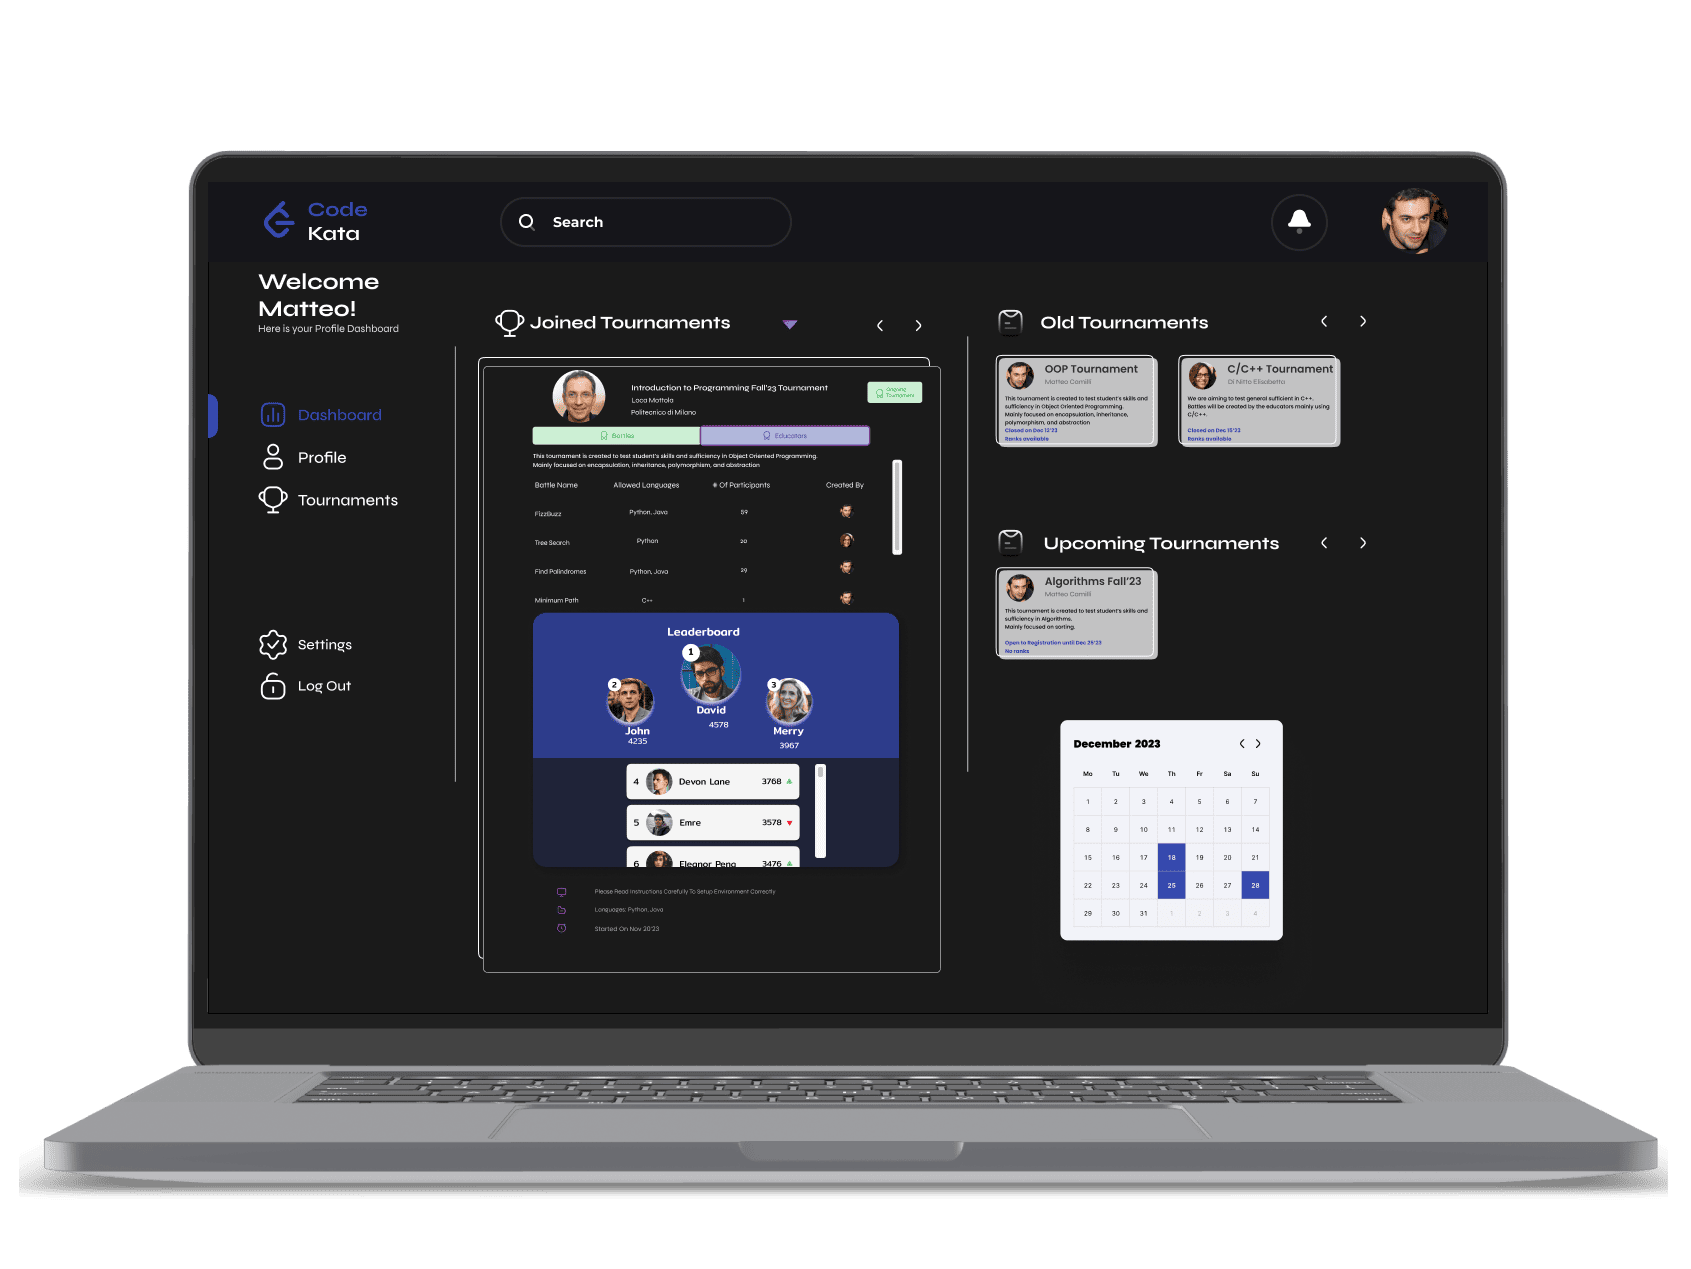
\includegraphics[scale=0.13]{Images/ui-ux/educator_dashboard/educator_dashboard_2.png}
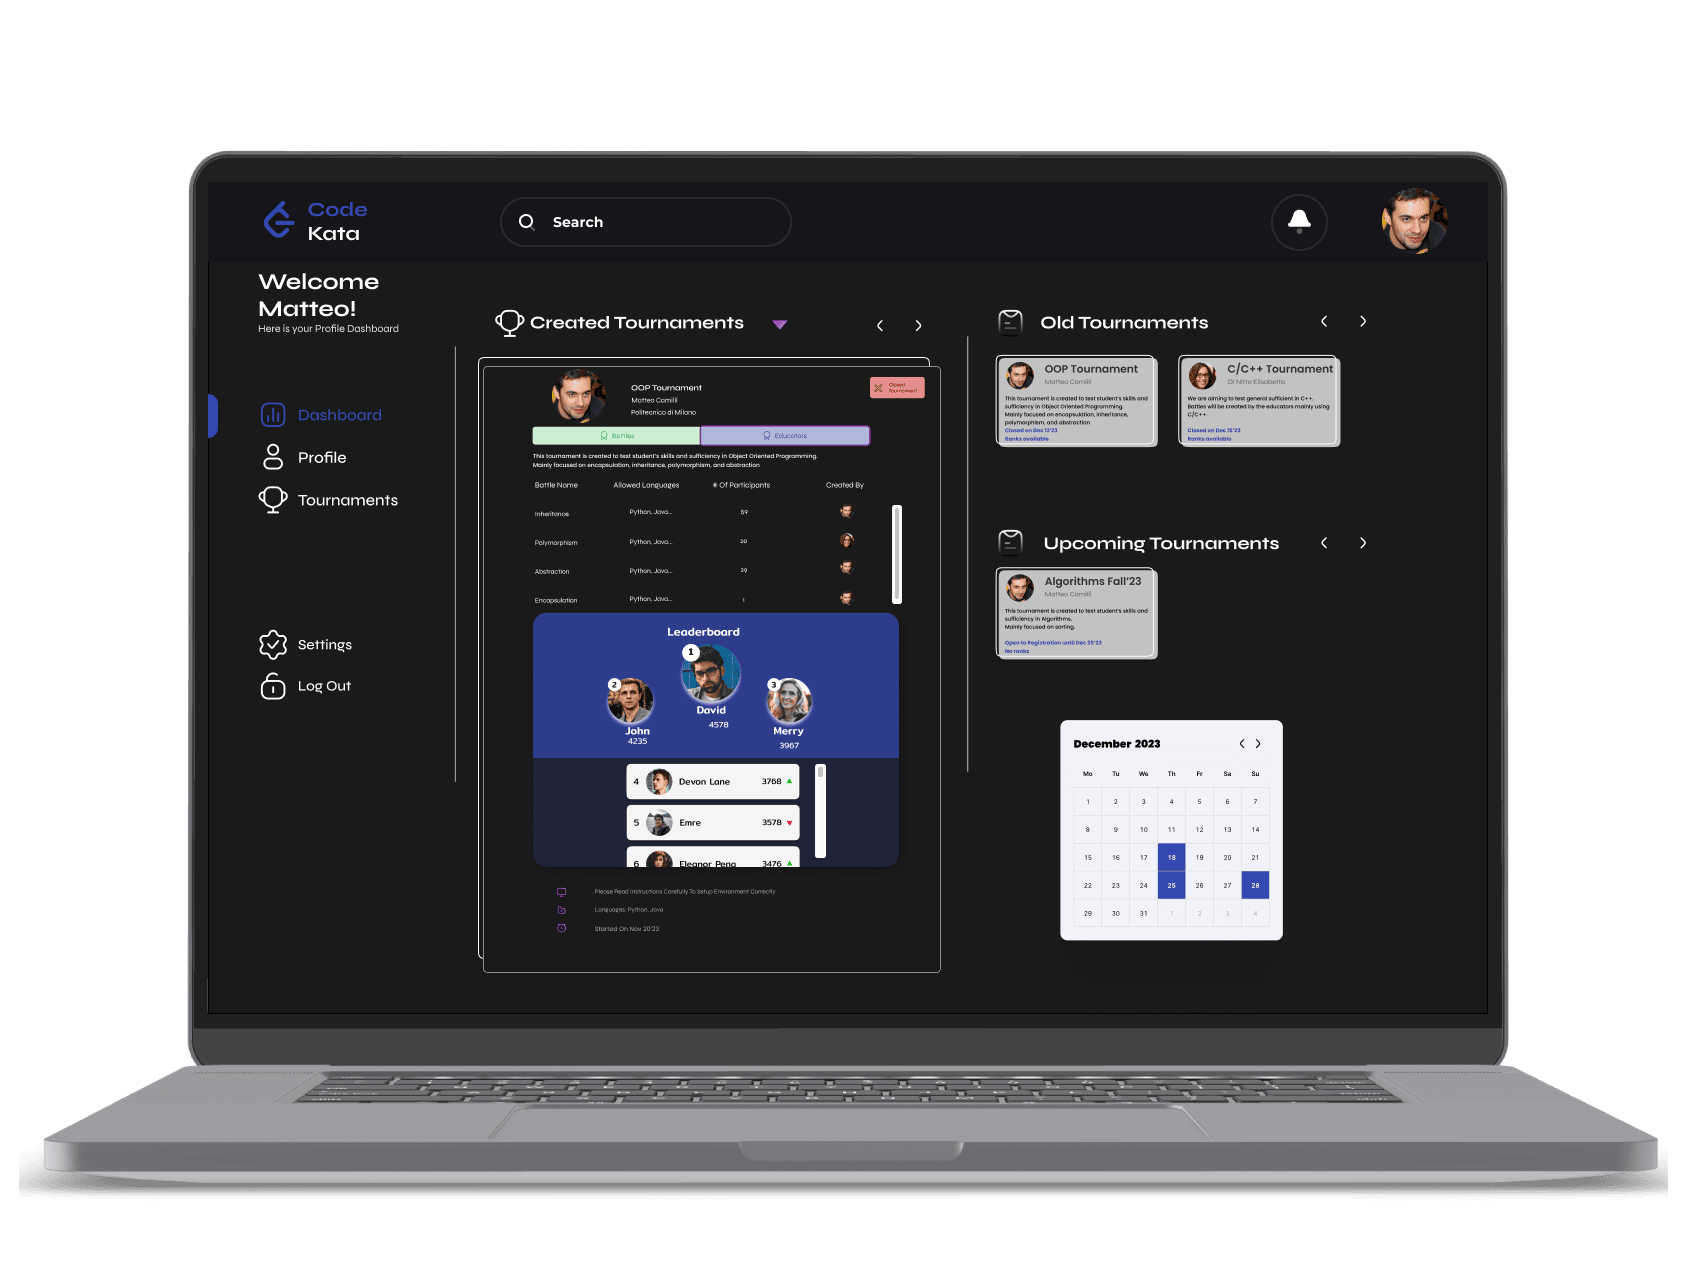
\includegraphics[scale=0.13]{Images/ui-ux/educator_dashboard/educator_dashboard_3.png}
\\ (i) Educator Dashboard
\end{center}
\begin{center}
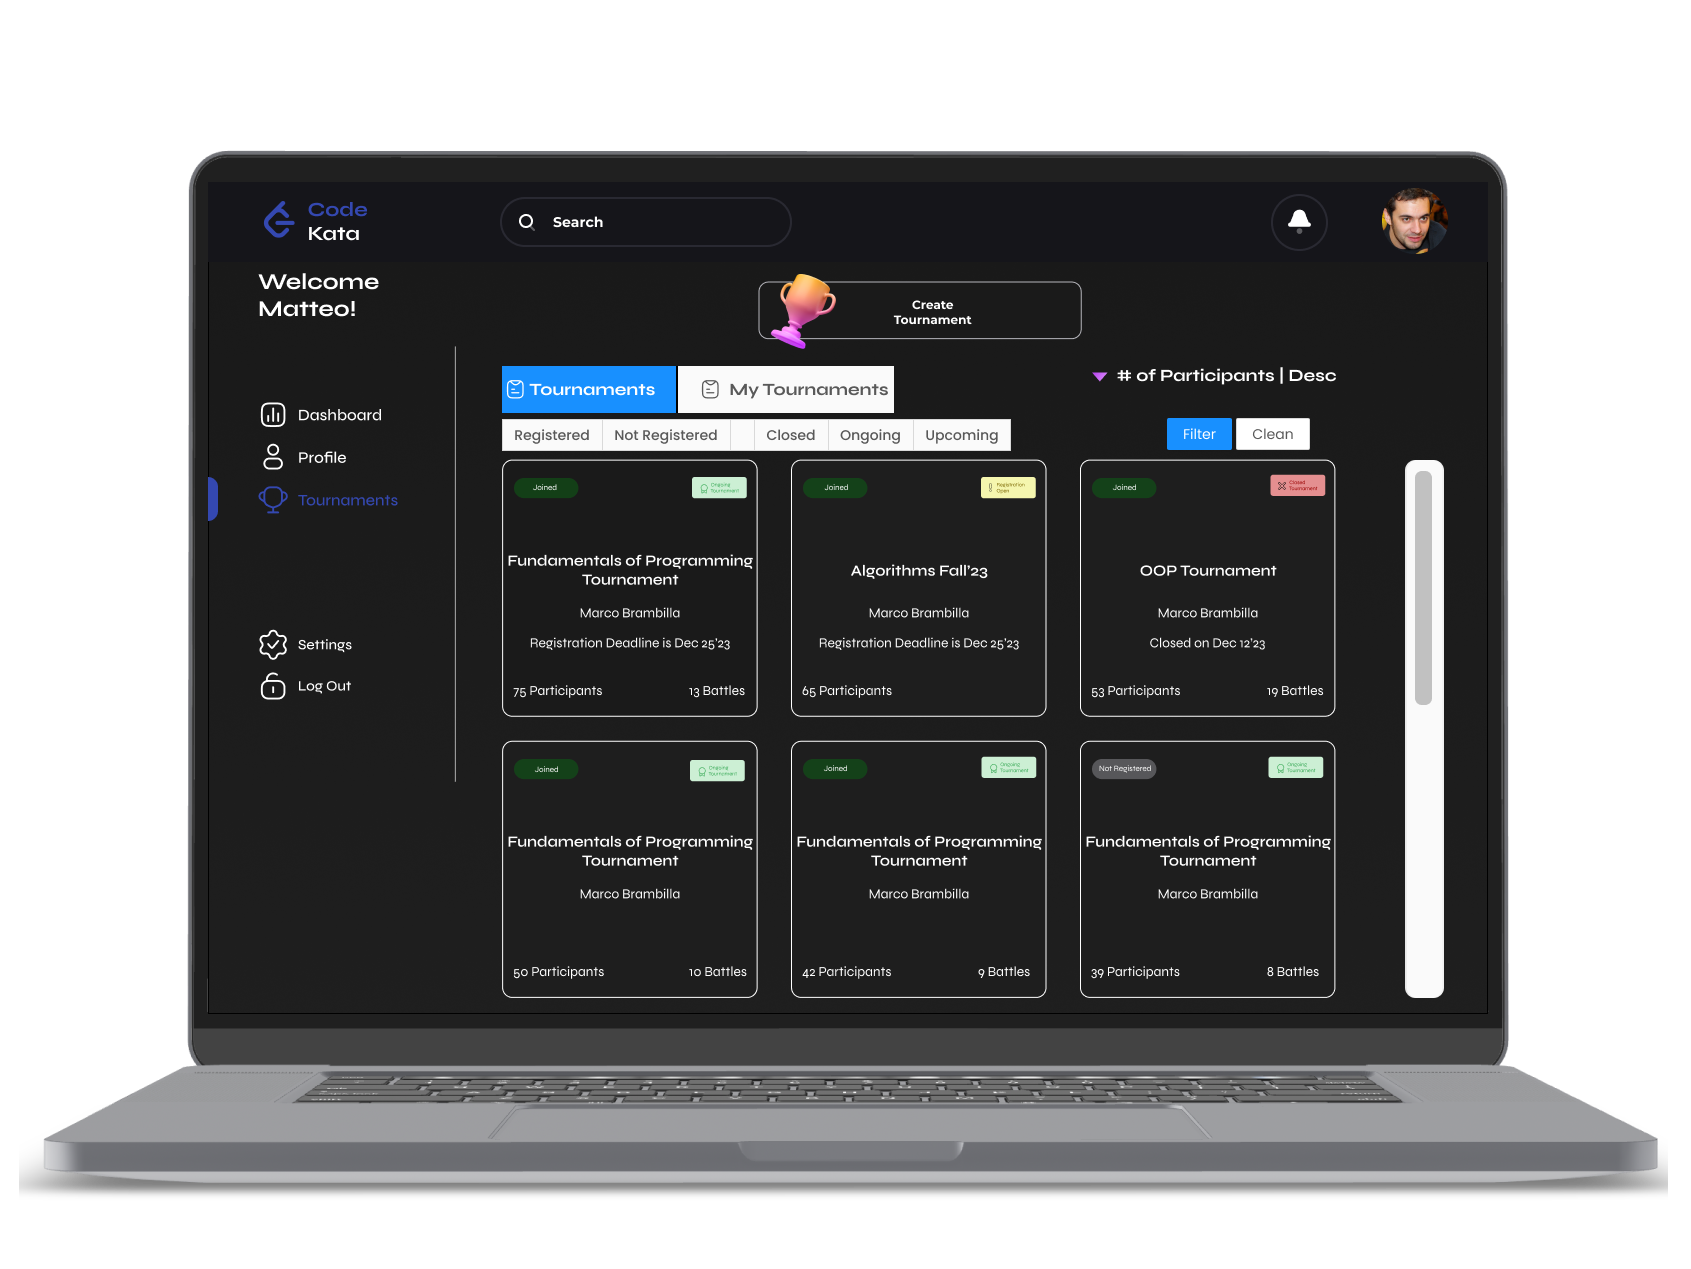
\includegraphics[scale=0.13]{Images/ui-ux/educator_tournaments/educator_tournaments_1.png}
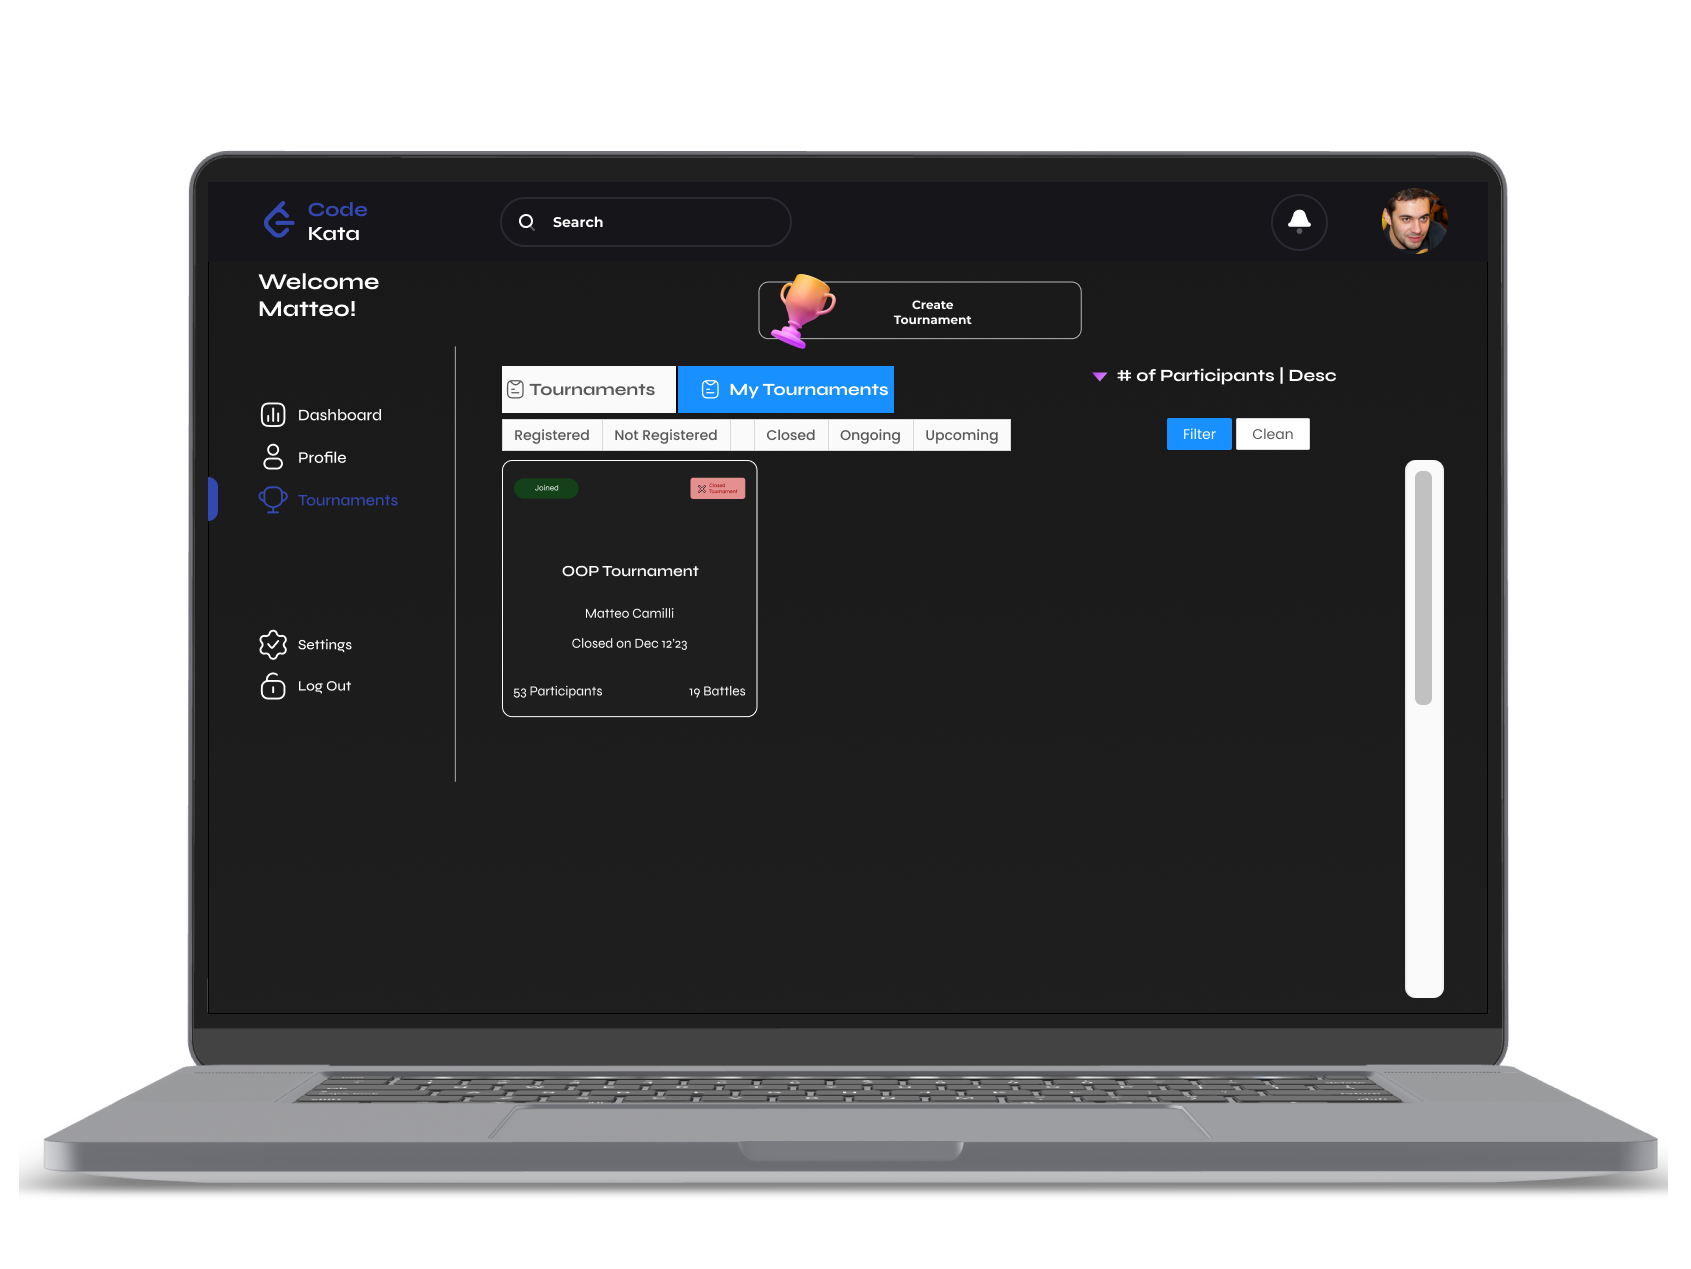
\includegraphics[scale=0.13]{Images/ui-ux/educator_tournaments/educator_tournaments_2.png}
        (j) Educator Tournaments
\end{center}
\begin{center}
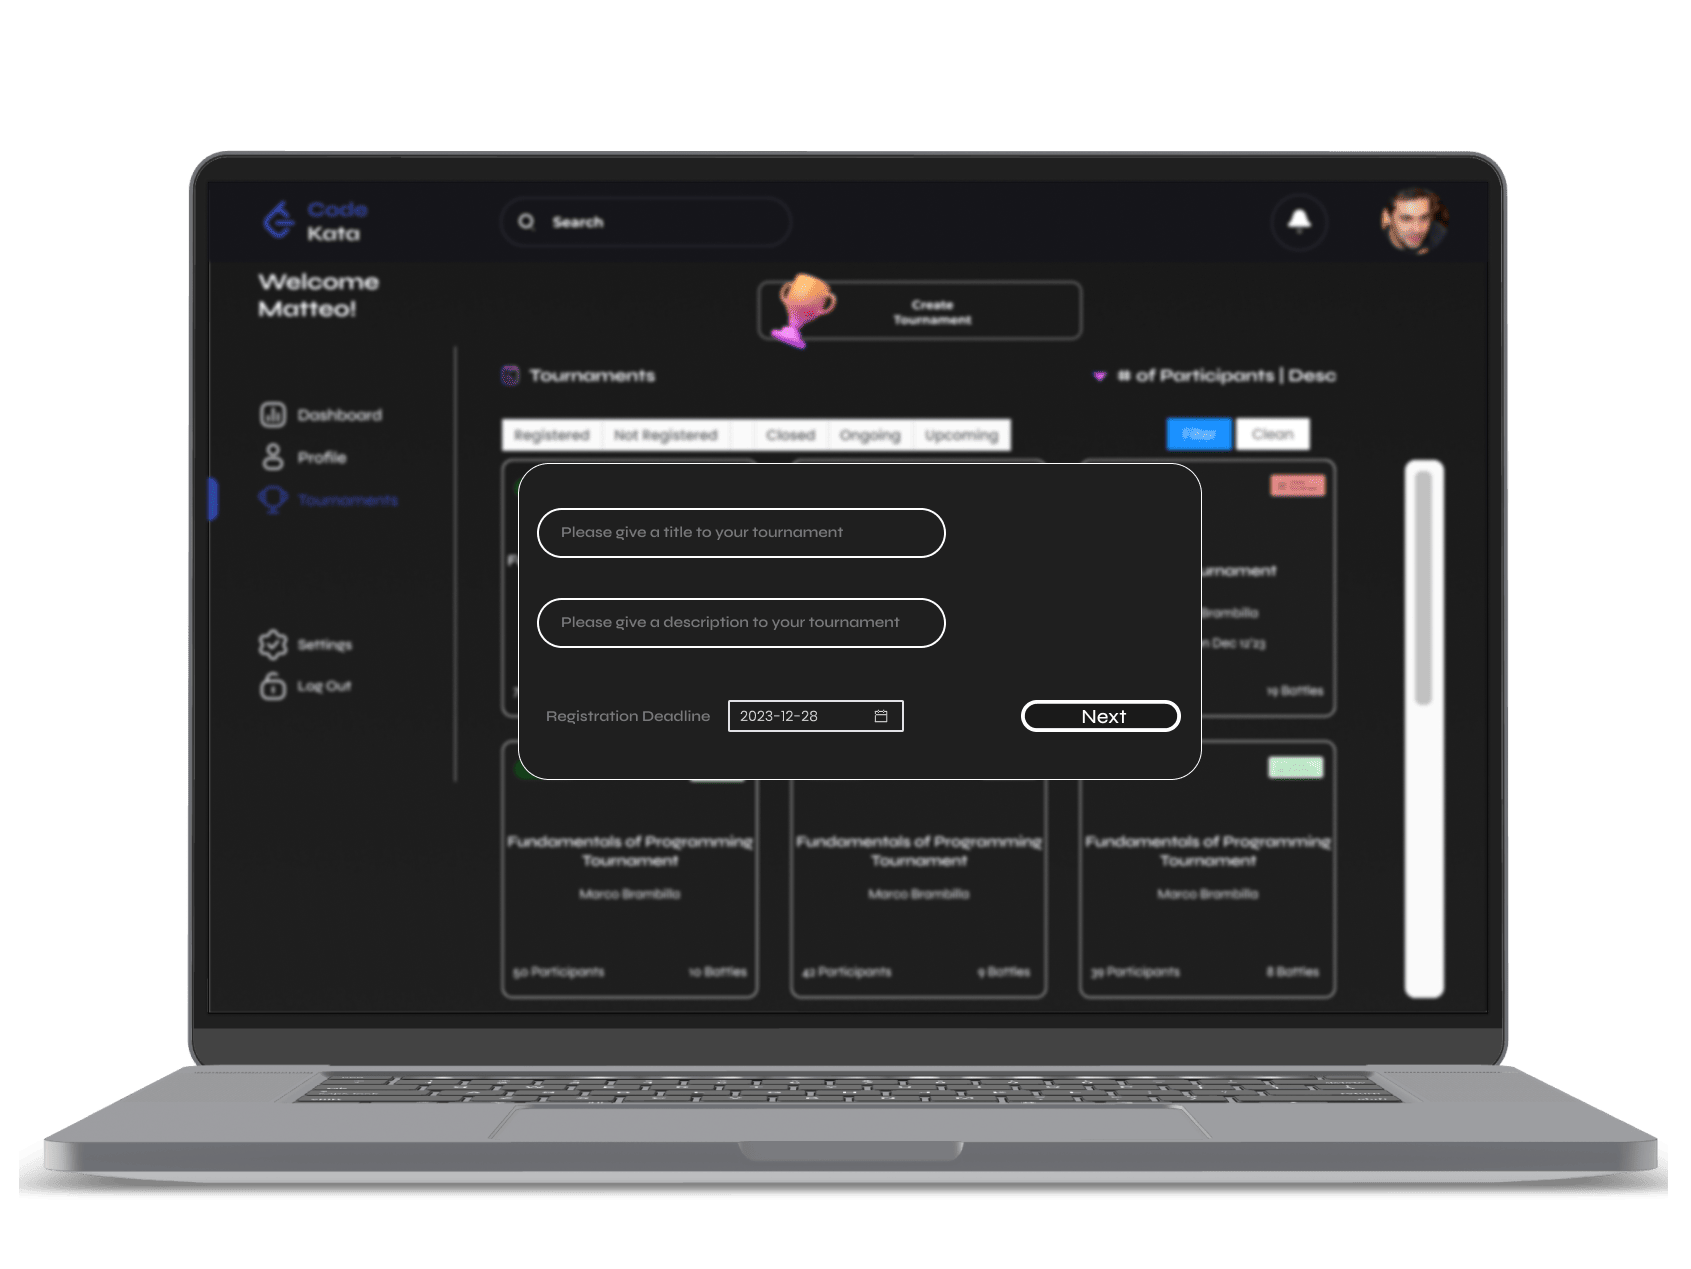
\includegraphics[scale=0.13]{Images/ui-ux/educator_create_tournament/educator_create_tournament_1.png}
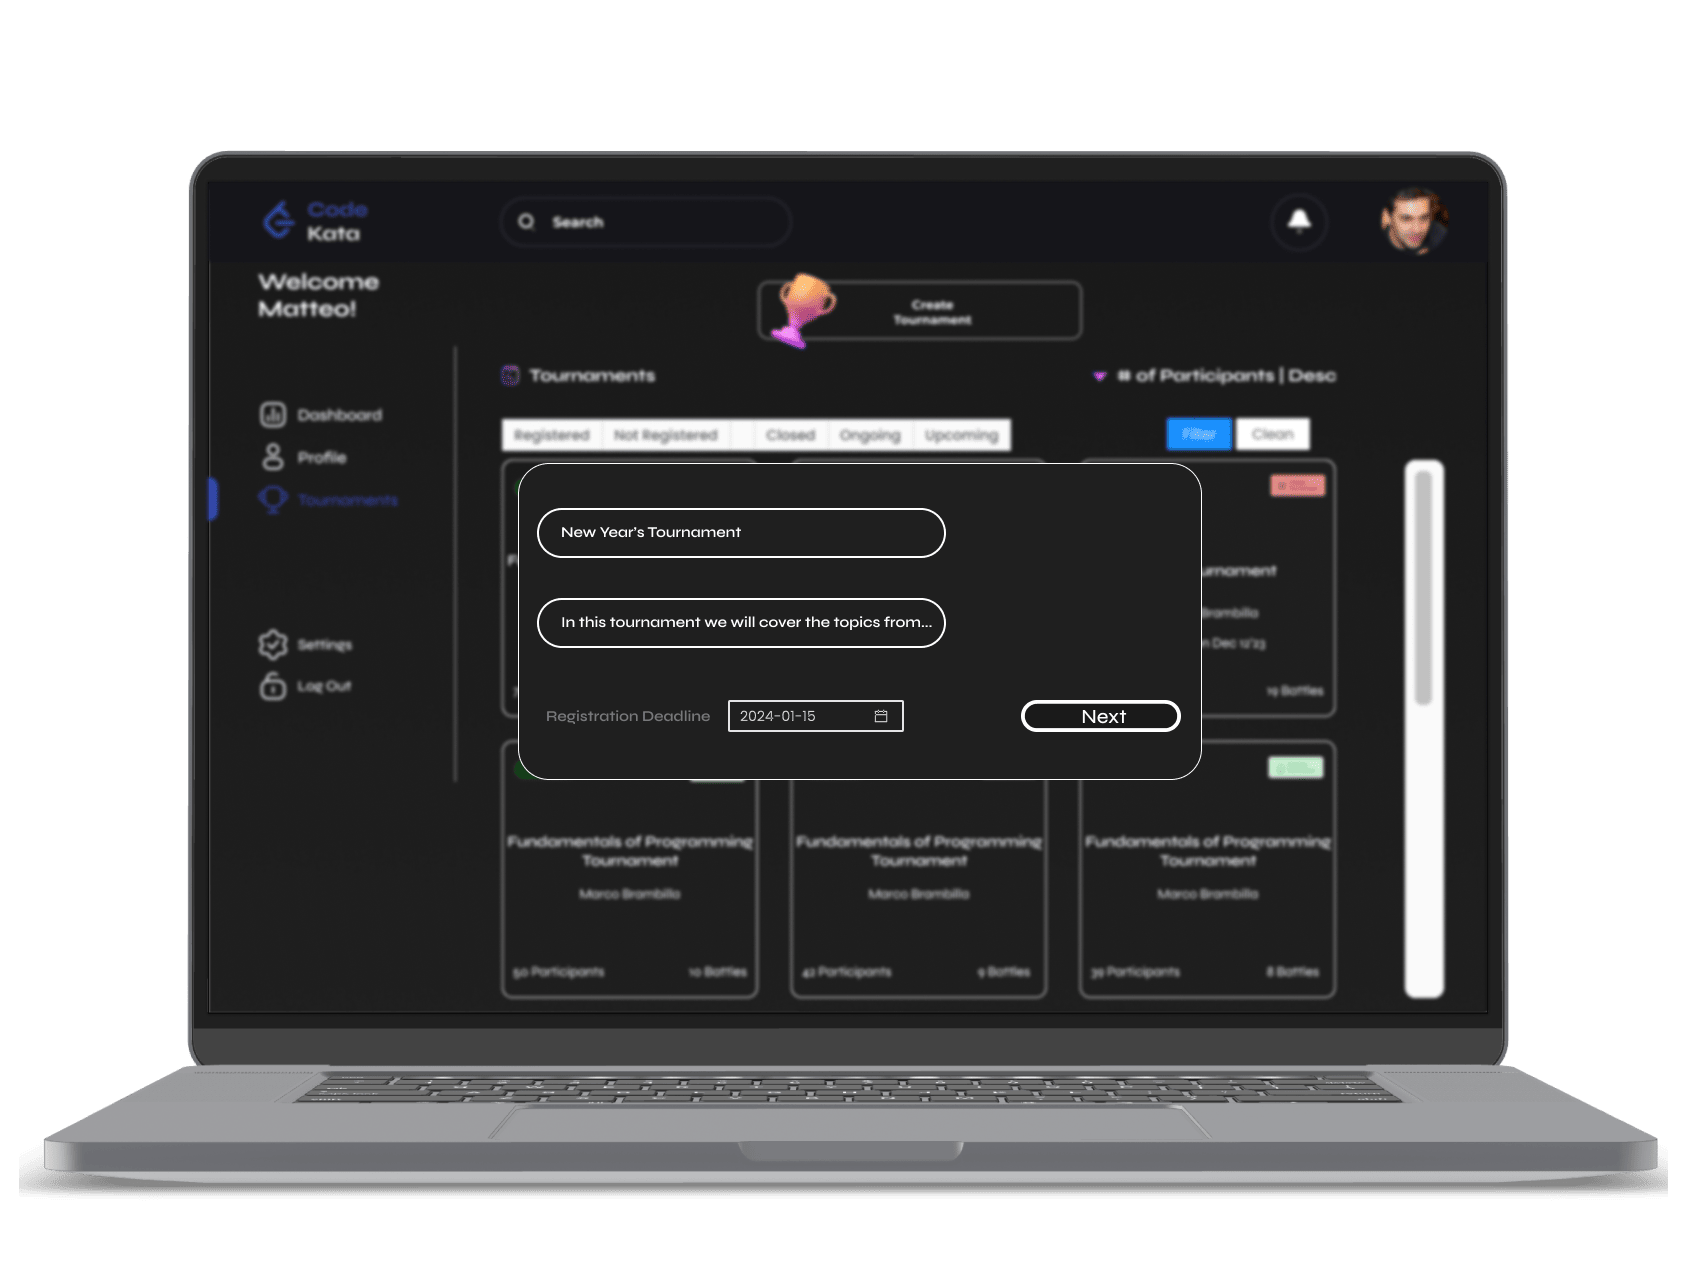
\includegraphics[scale=0.13]{Images/ui-ux/educator_create_tournament/educator_create_tournament_2.png}
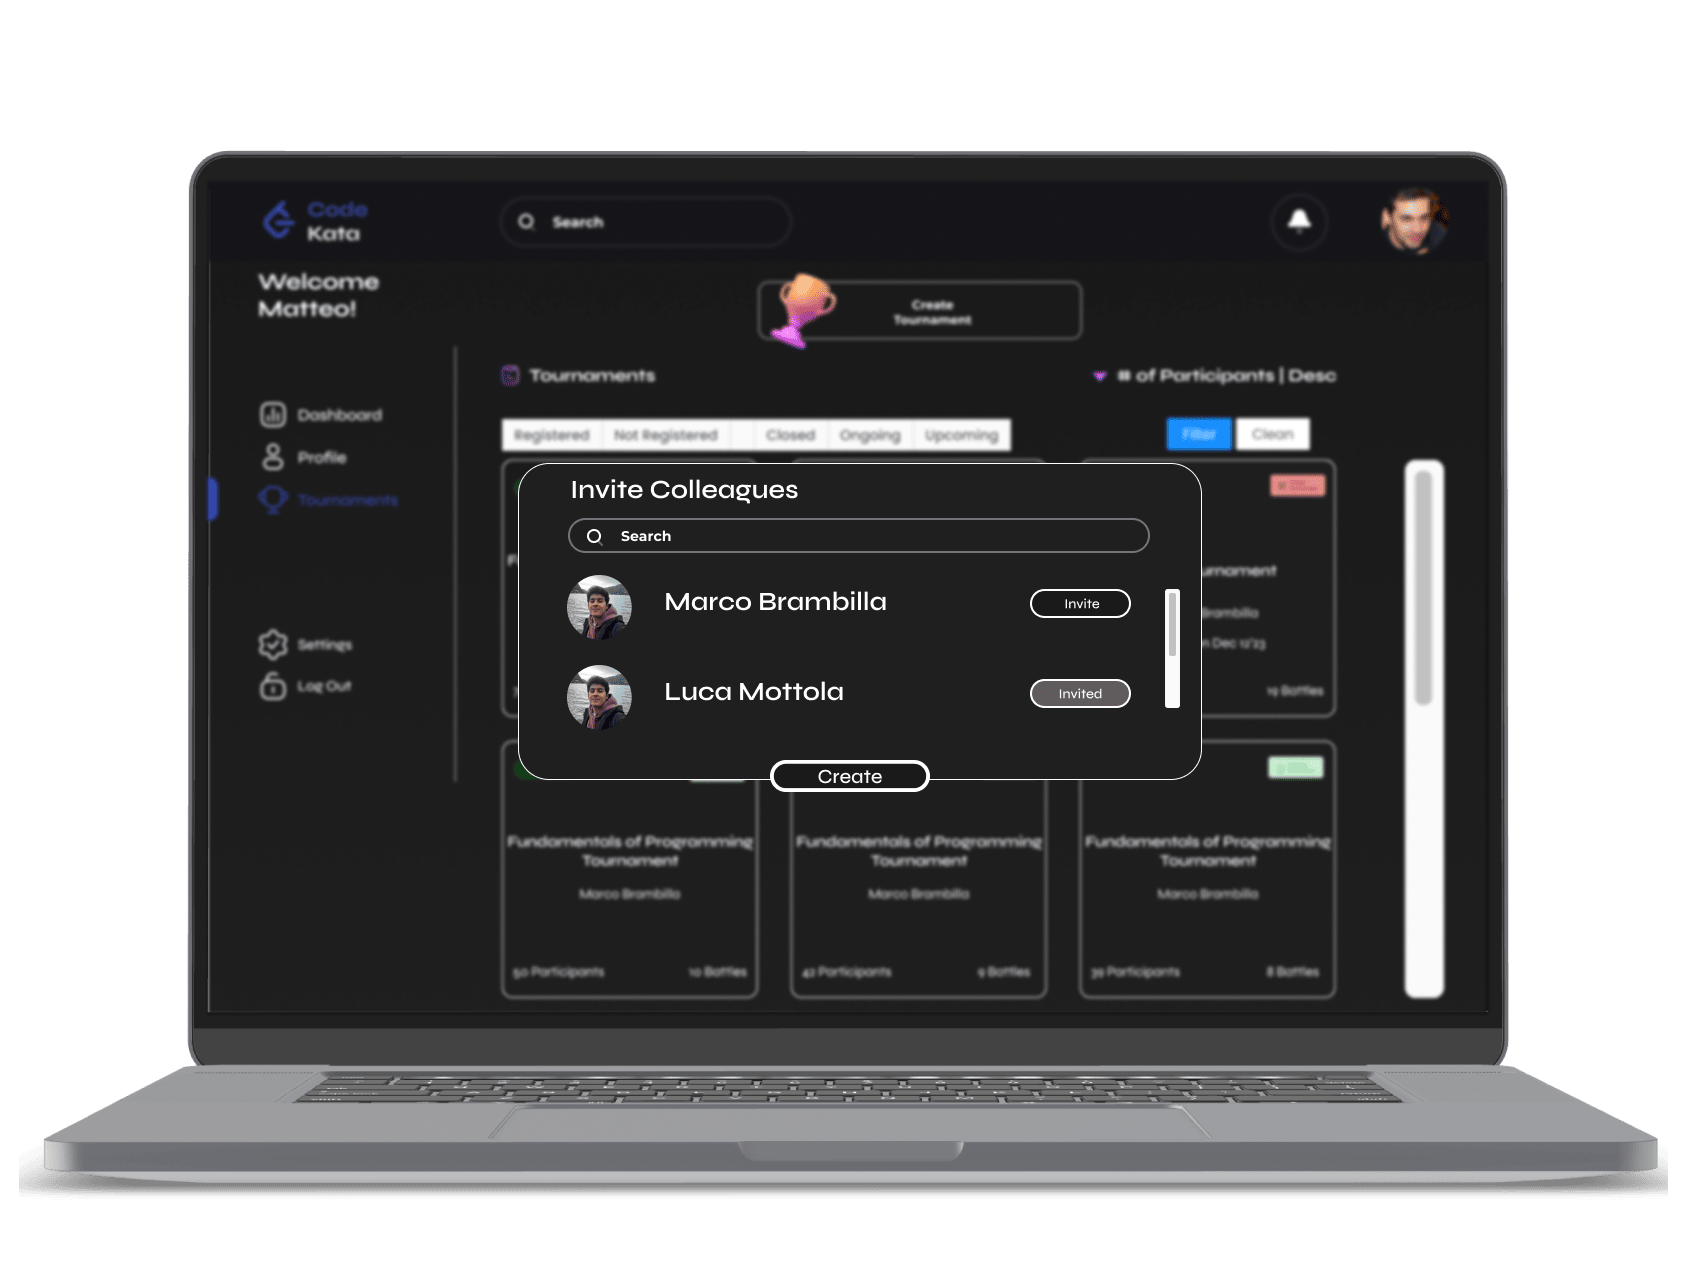
\includegraphics[scale=0.13]{Images/ui-ux/educator_create_tournament/educator_create_tournament_3.png}
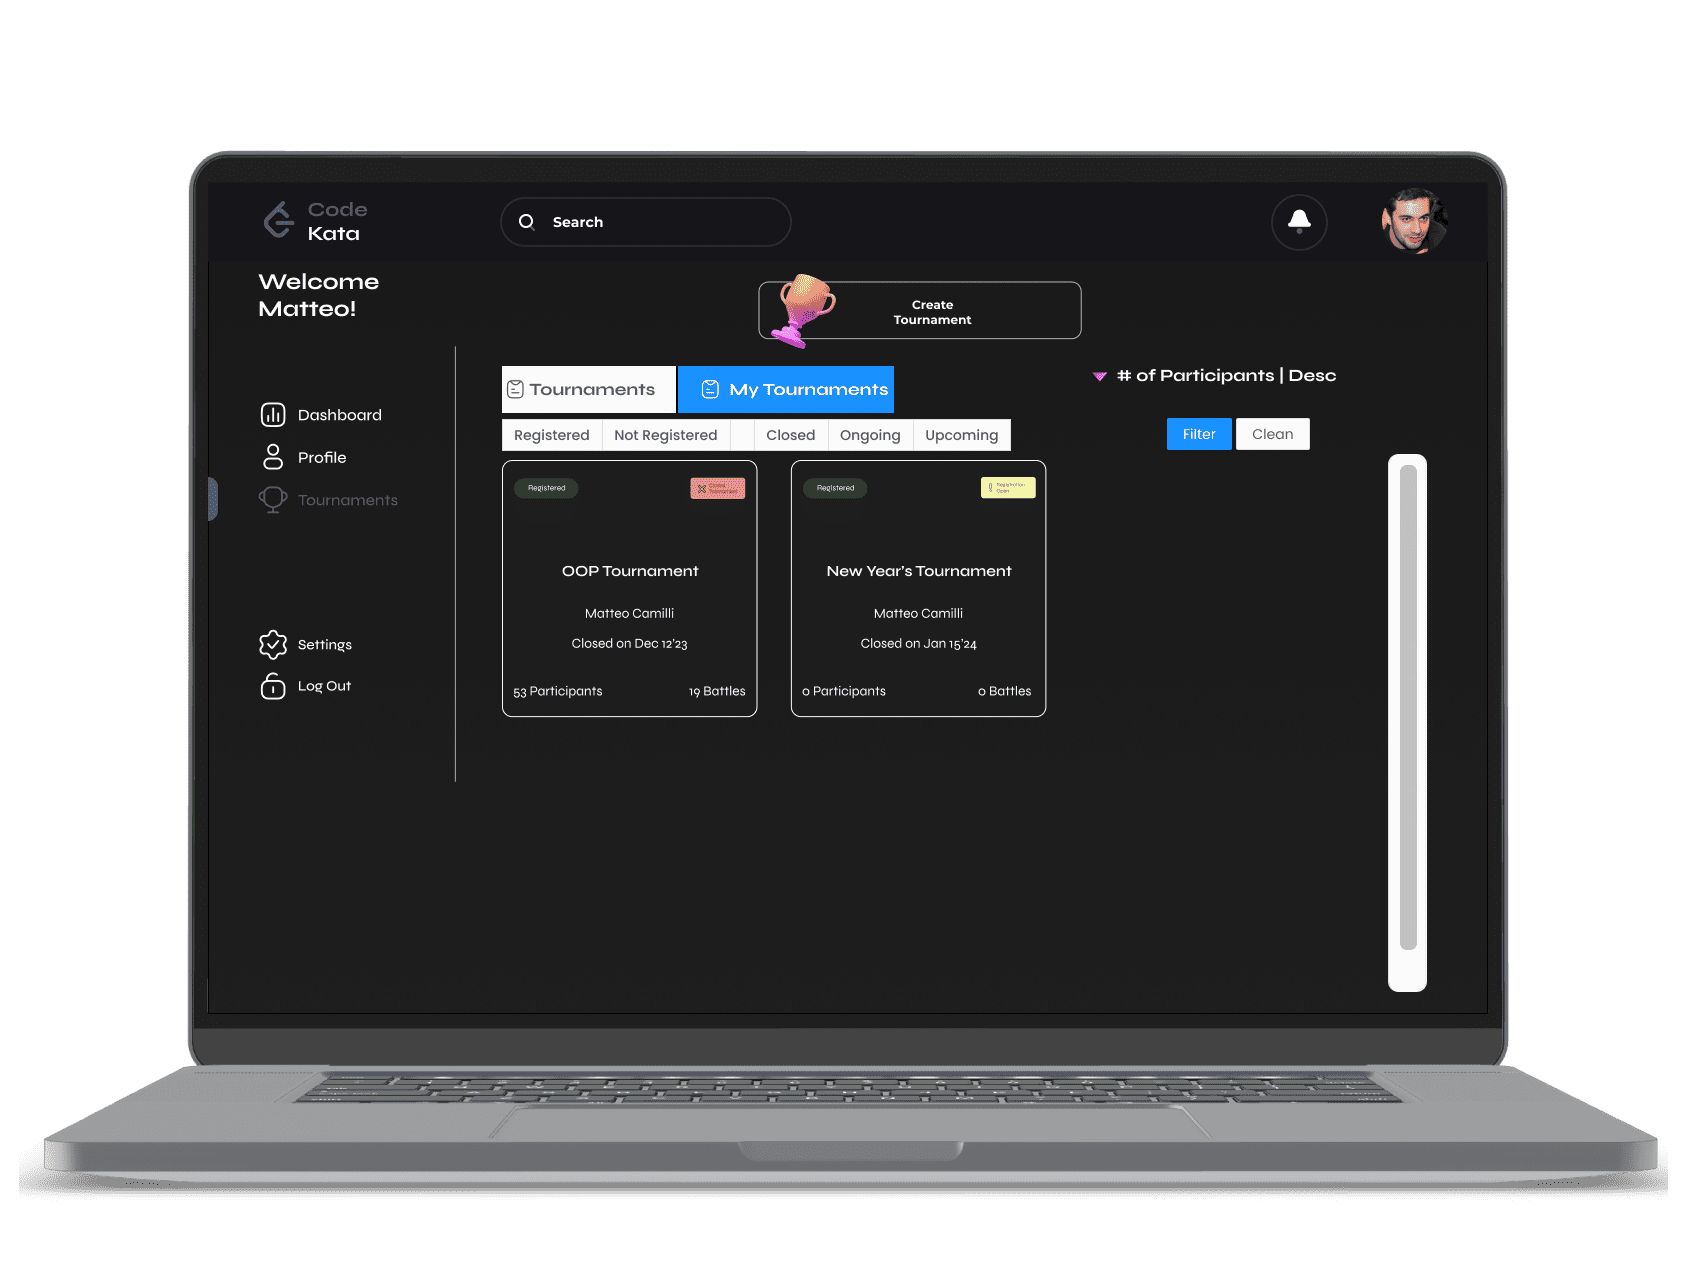
\includegraphics[scale=0.13]{Images/ui-ux/educator_create_tournament/educator_create_tournament_4.png}
        (k) Educator Creates Tournament
\end{center}
\newpage
\begin{center}
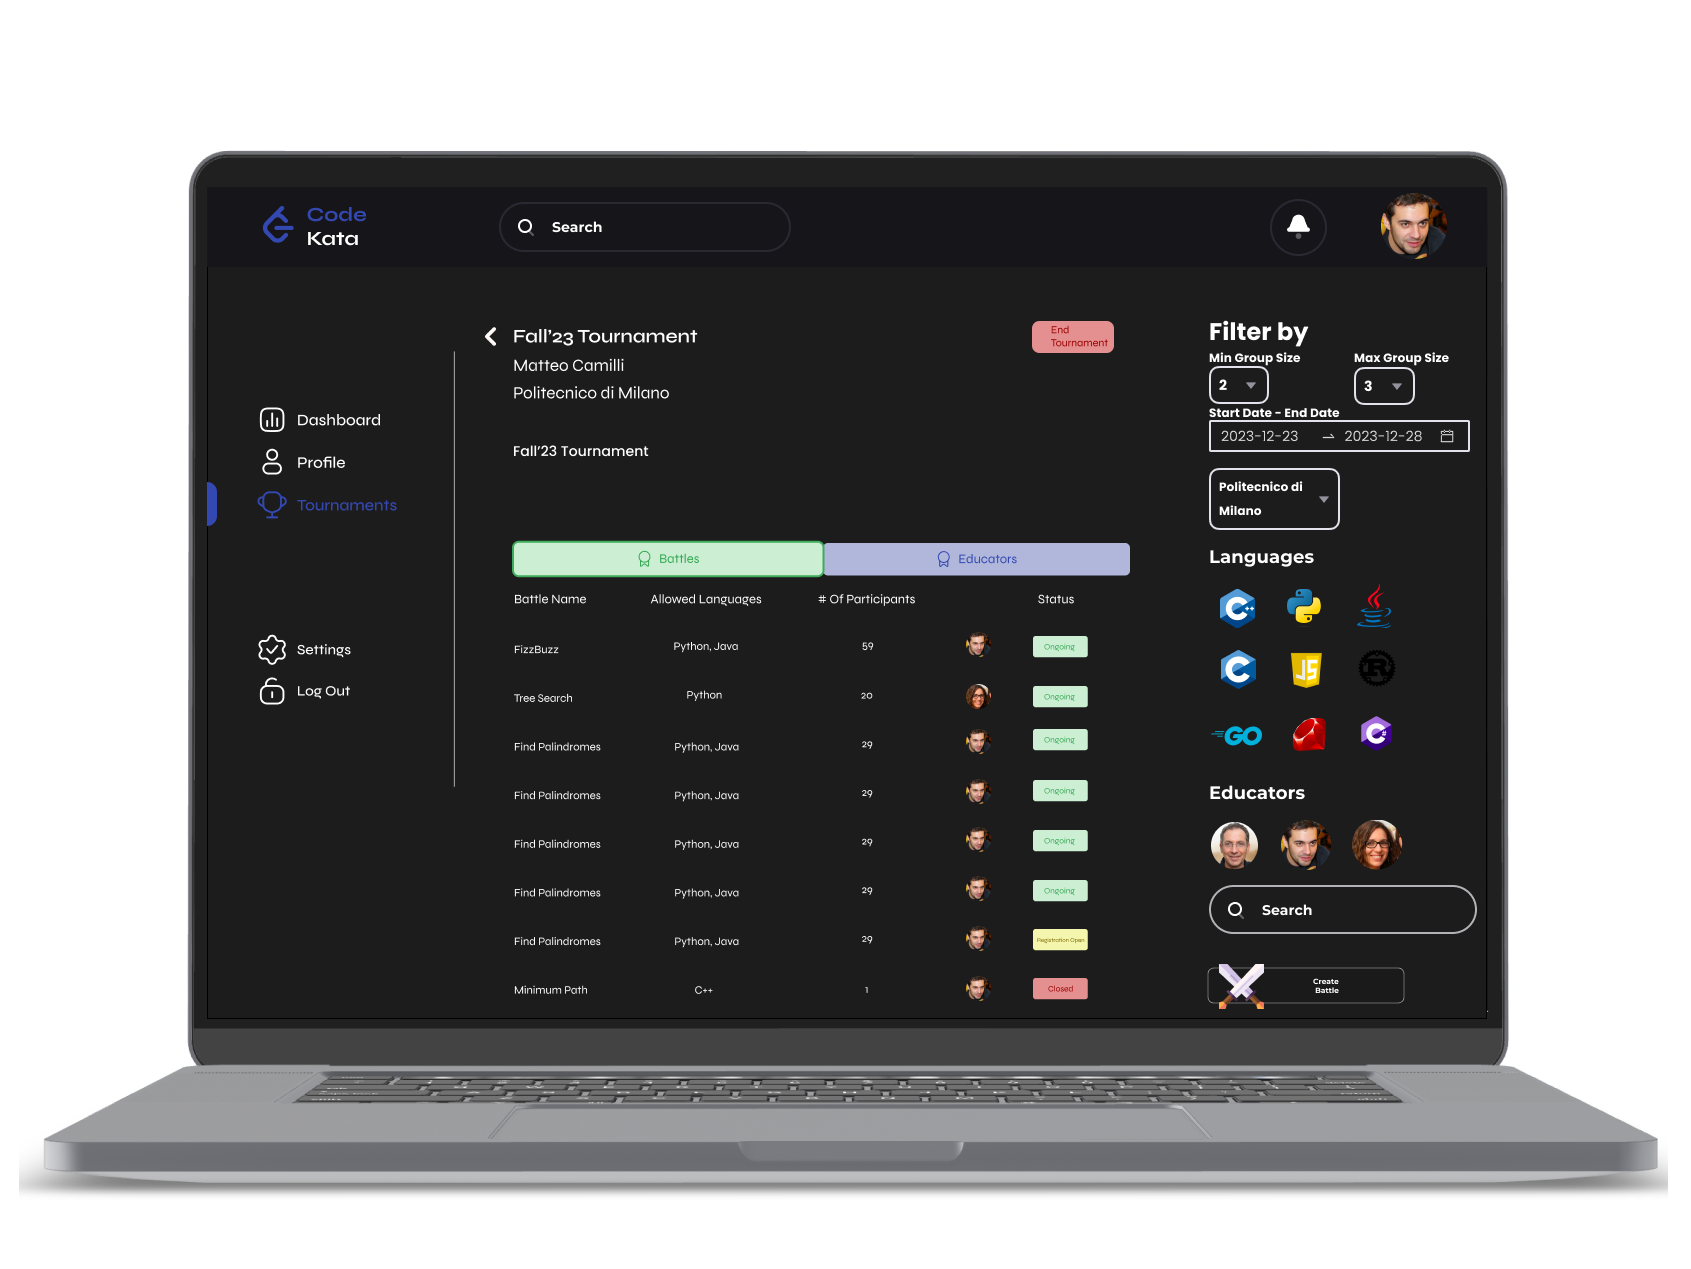
\includegraphics[scale=0.13]{Images/ui-ux/educator_creates_battle/educator_creates_battle_1.png}
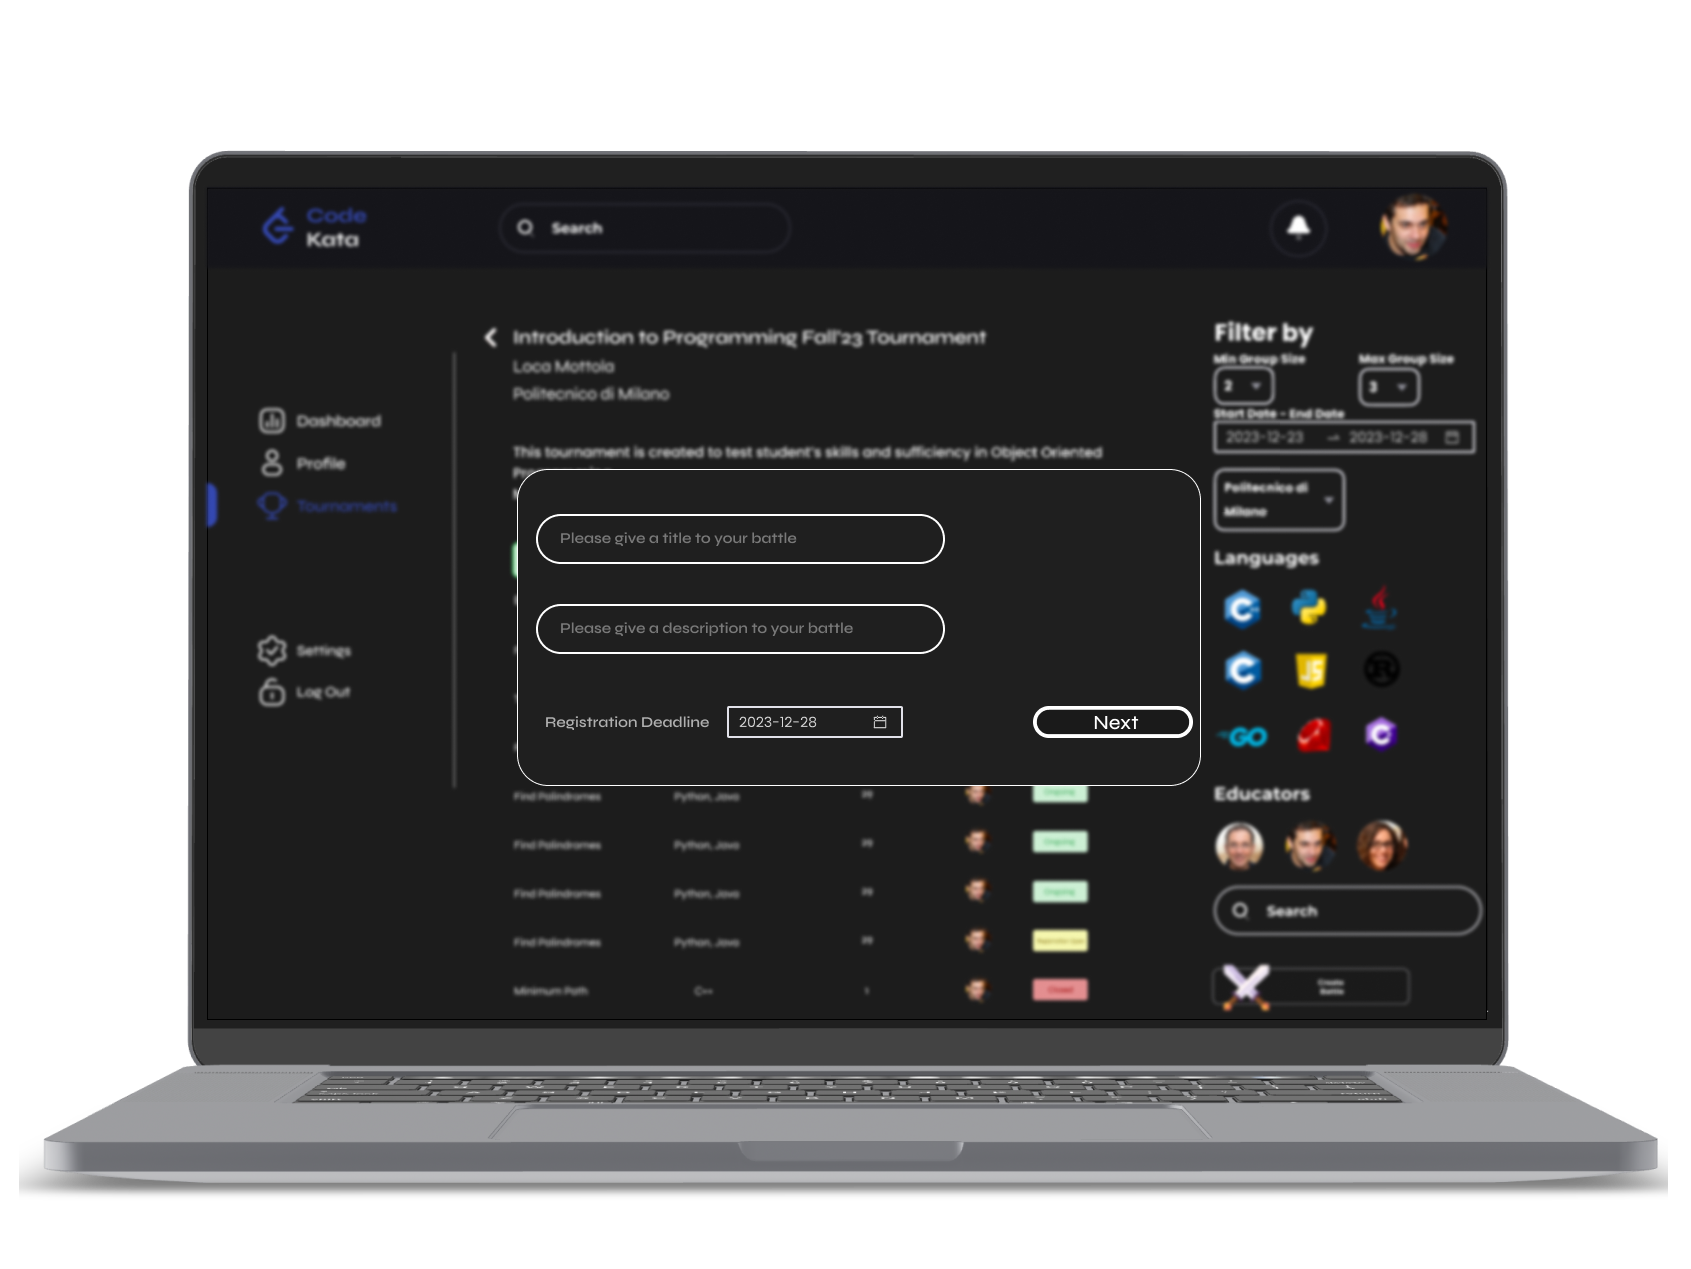
\includegraphics[scale=0.13]{Images/ui-ux/educator_creates_battle/educator_creates_battle_2.png}
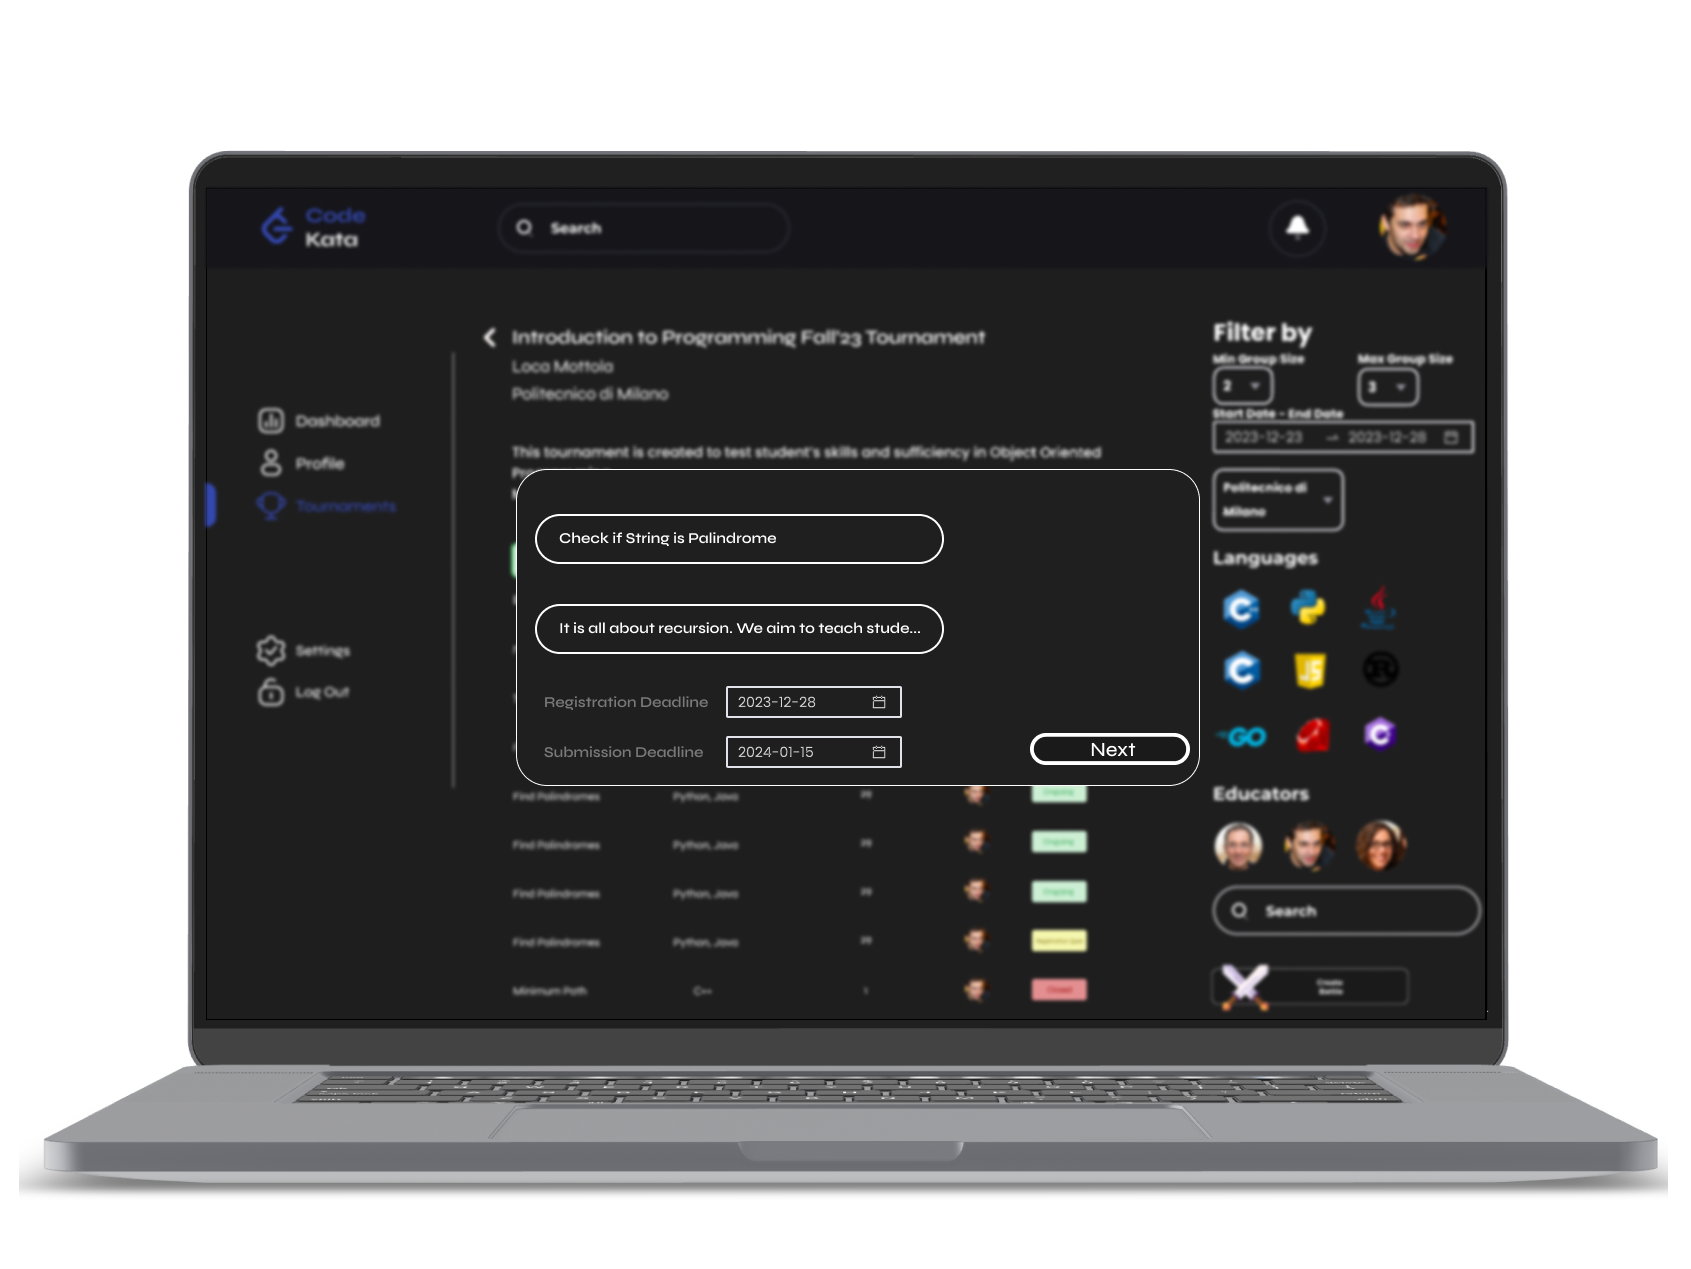
\includegraphics[scale=0.13]{Images/ui-ux/educator_creates_battle/educator_creates_battle_3.png}
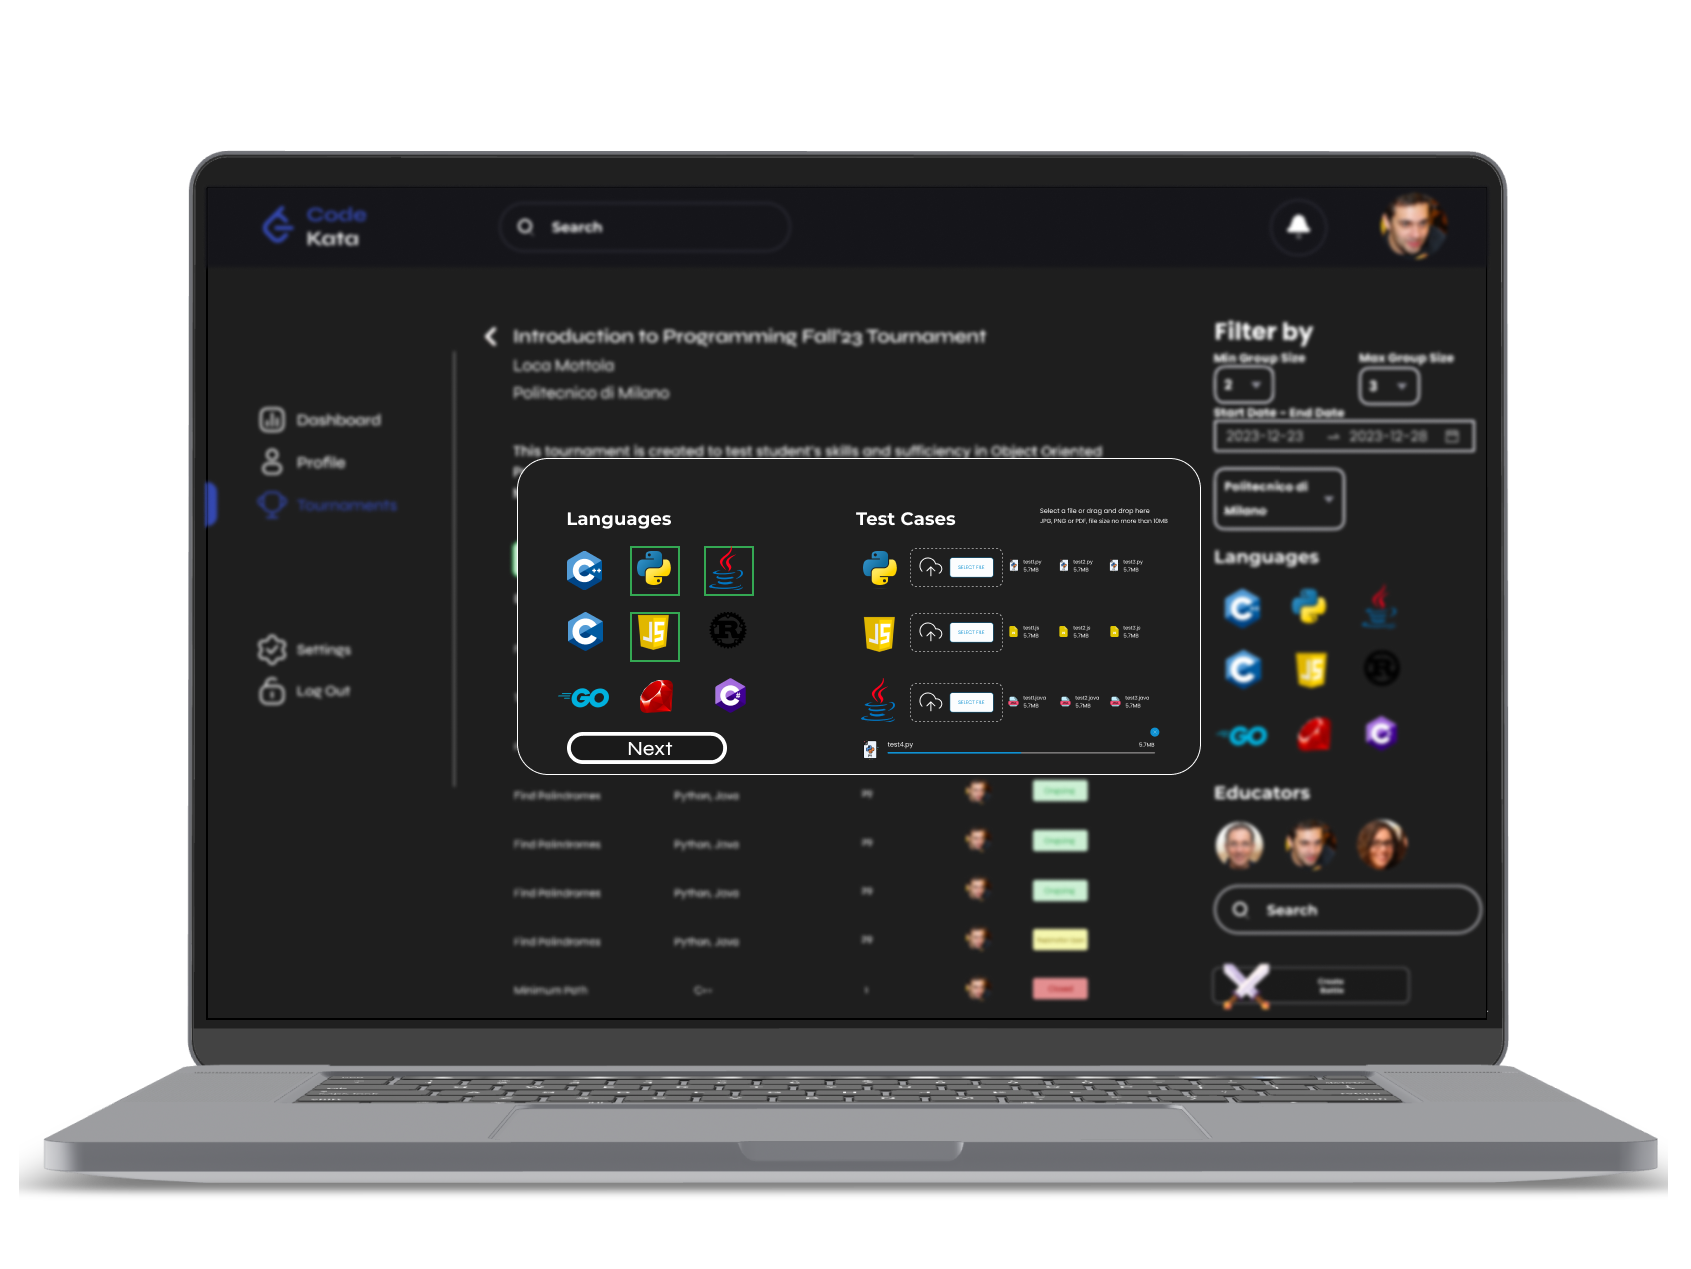
\includegraphics[scale=0.13]{Images/ui-ux/educator_creates_battle/educator_creates_battle_4.png}
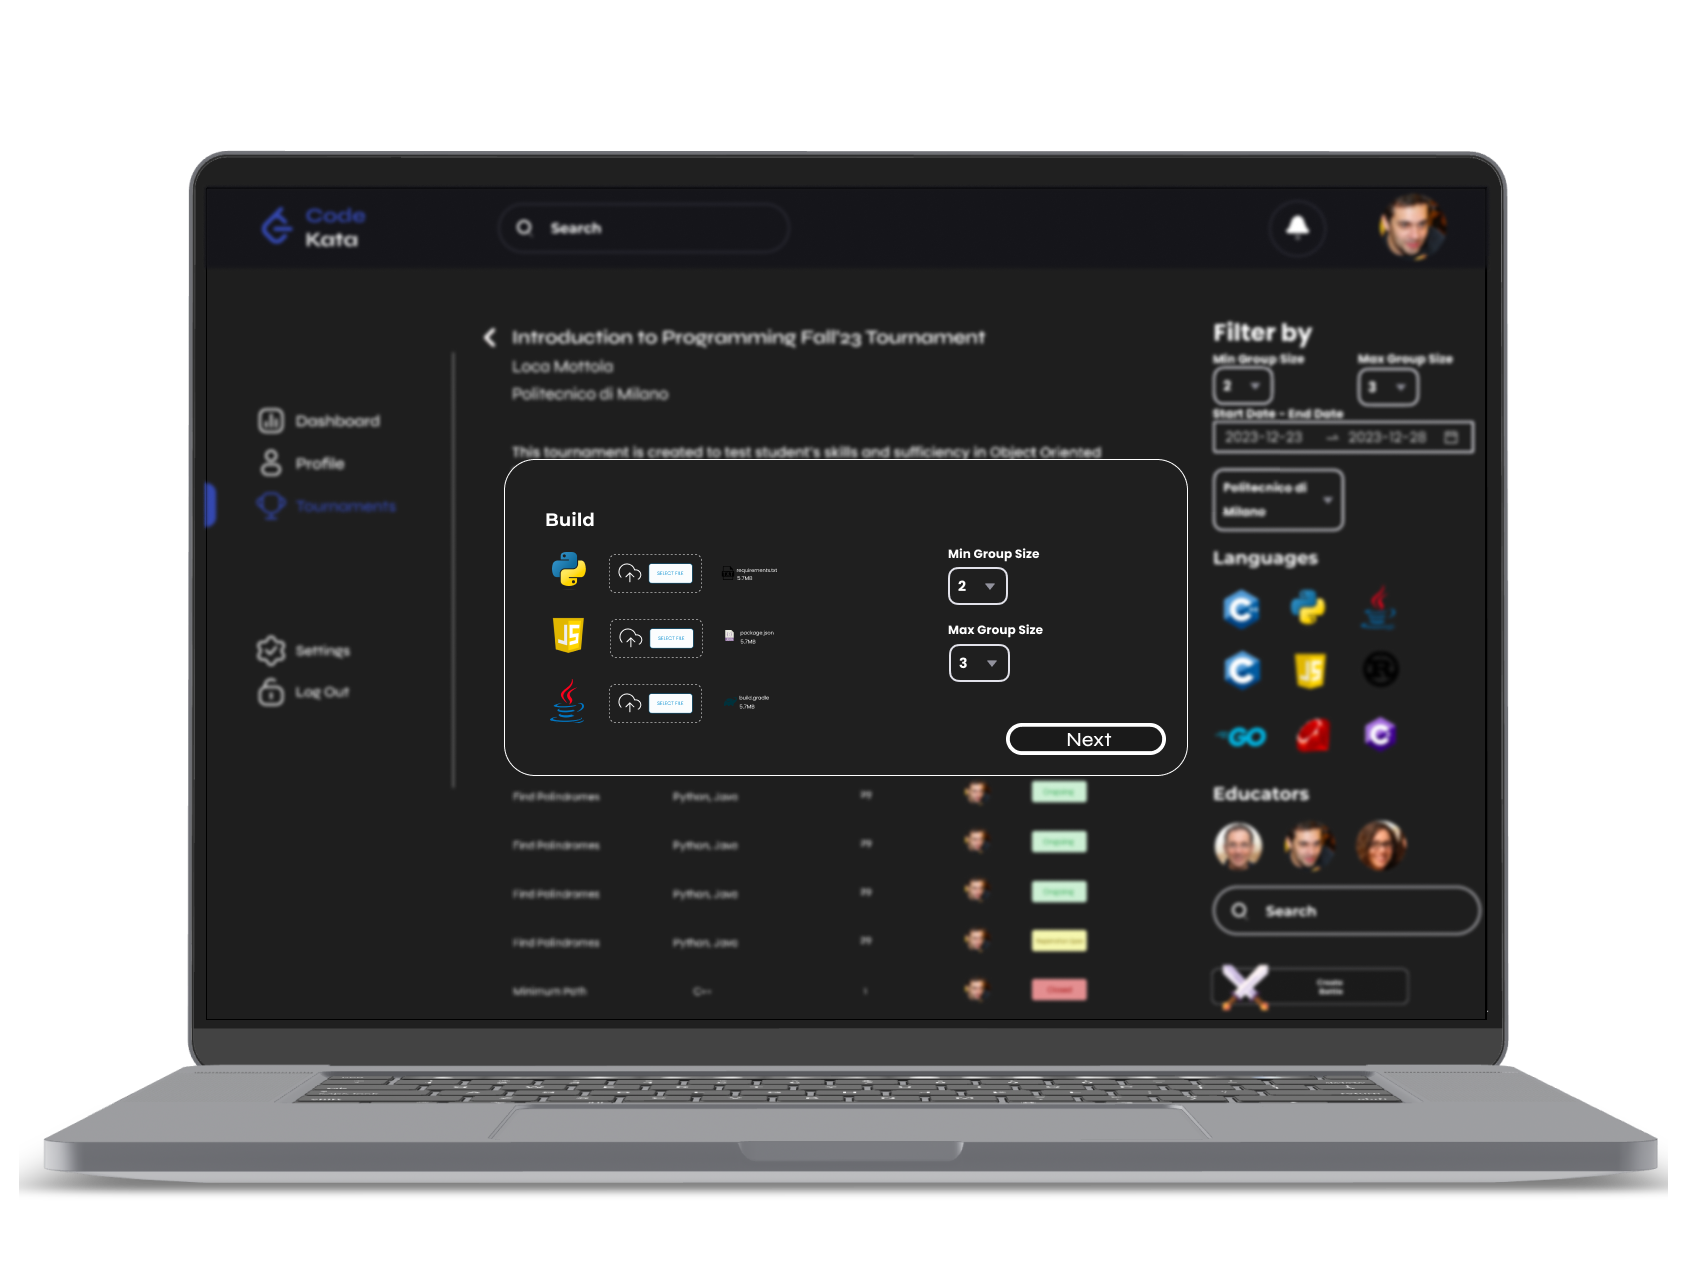
\includegraphics[scale=0.13]{Images/ui-ux/educator_creates_battle/educator_creates_battle_5.png}
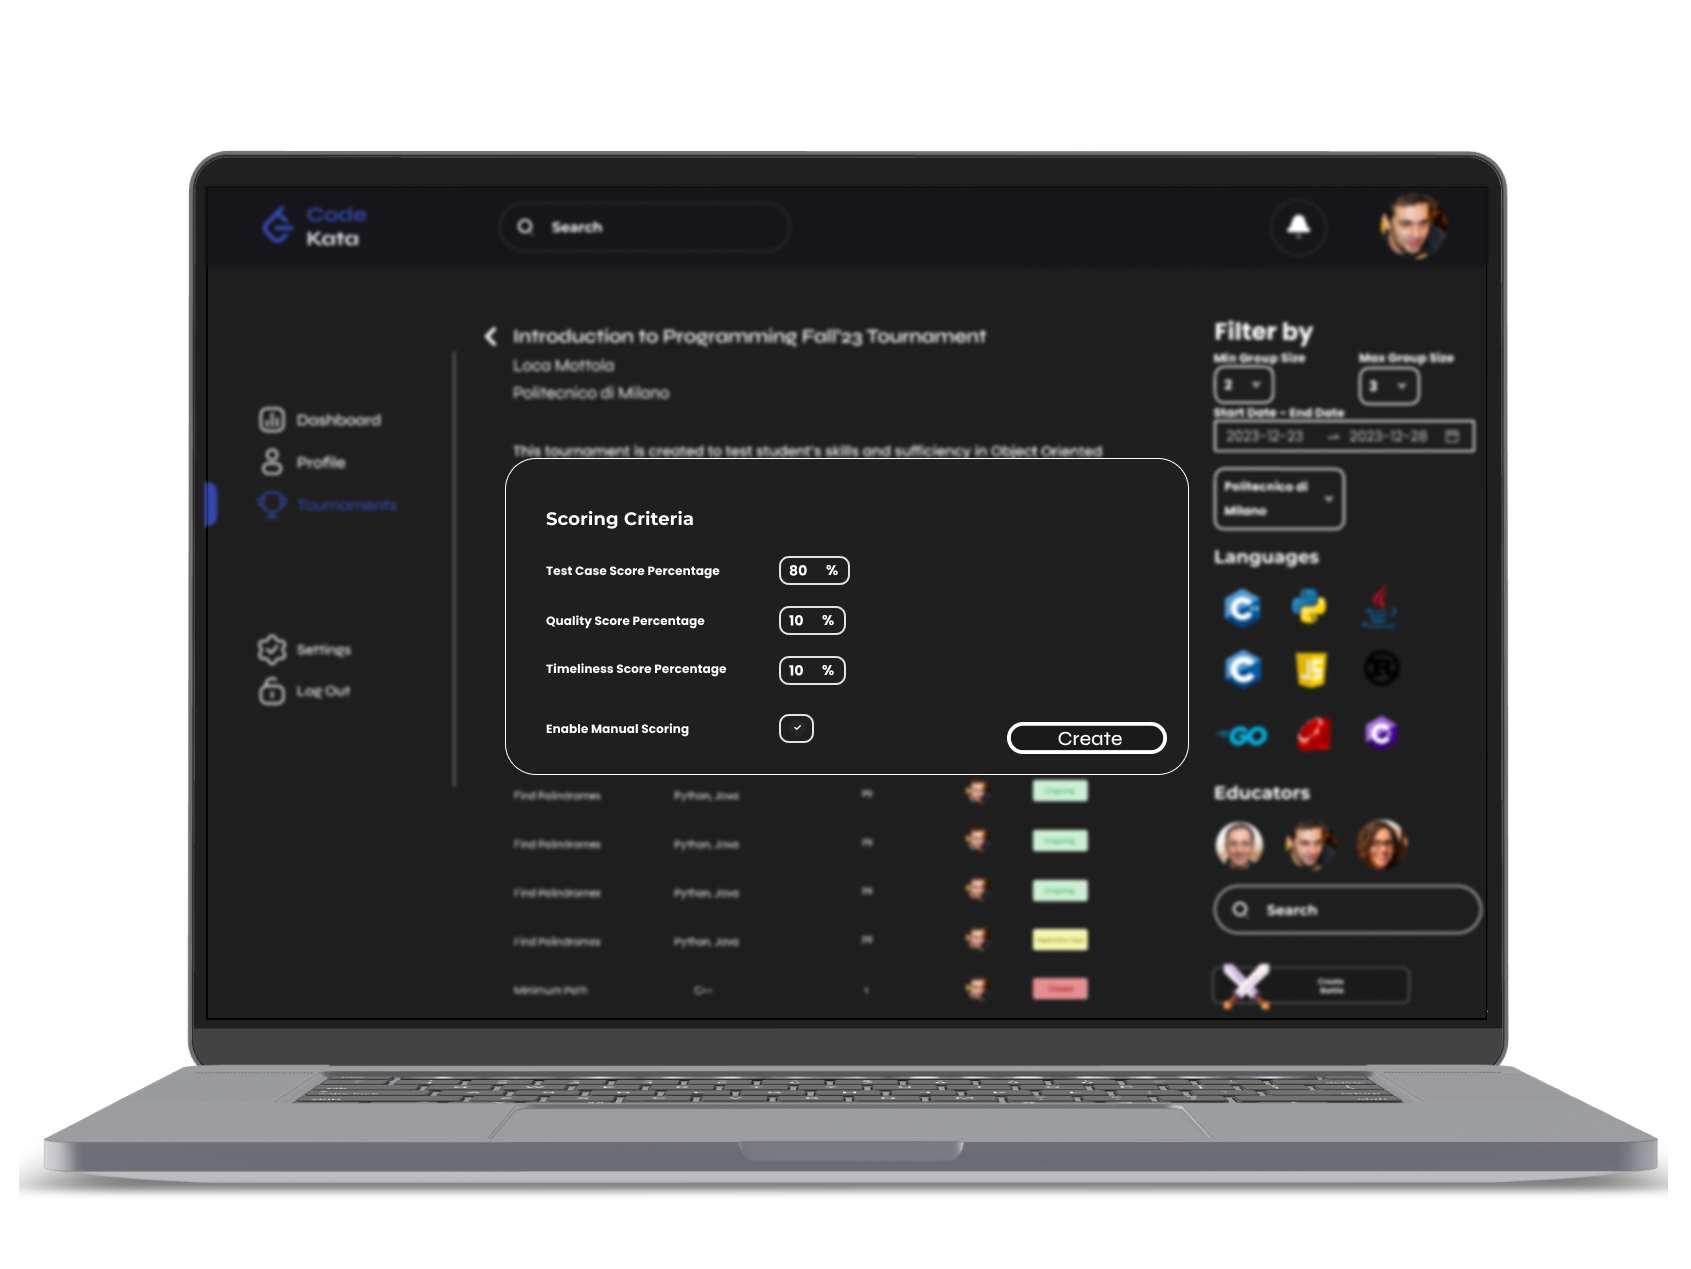
\includegraphics[scale=0.13]{Images/ui-ux/educator_creates_battle/educator_creates_battle_6.png}
        (l) Educator Creates Battle
\end{center}
\newpage
\begin{center}
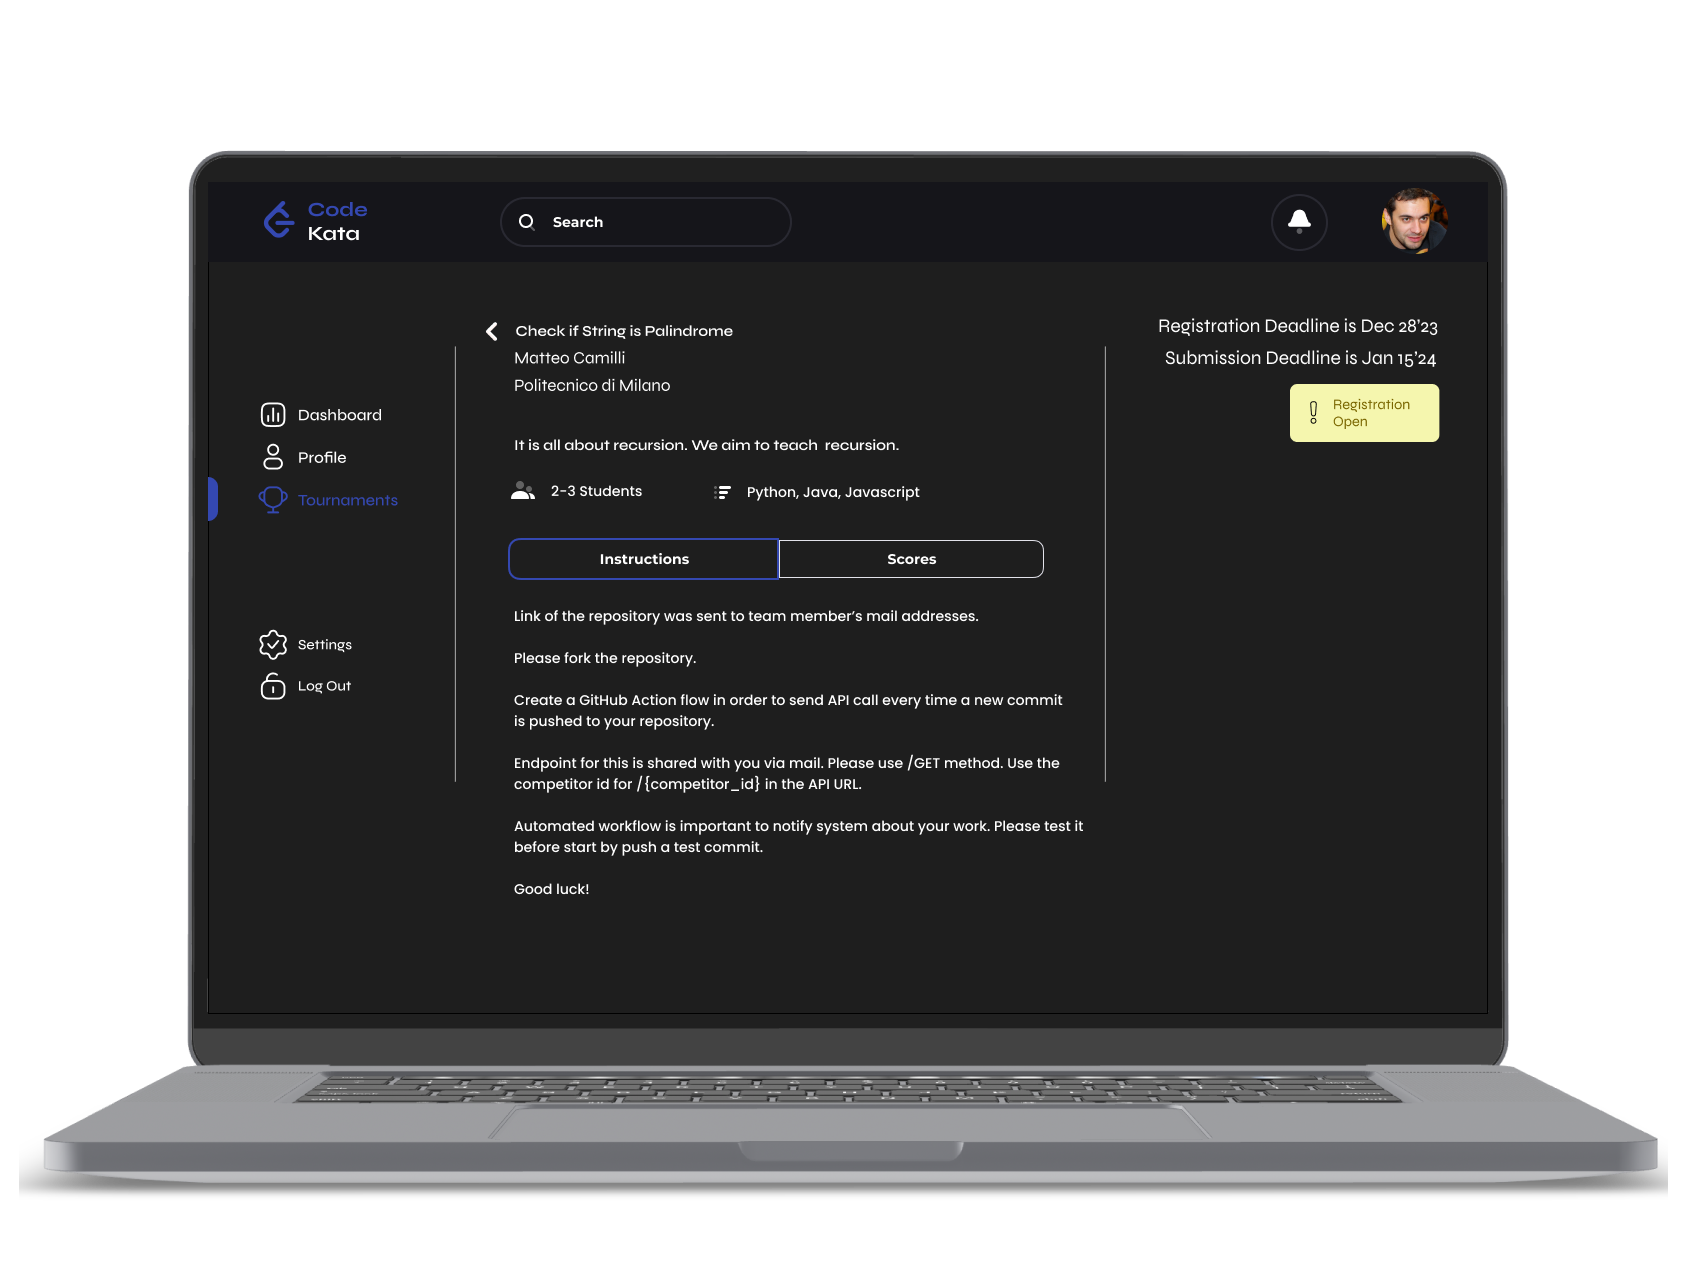
\includegraphics[scale=0.13]{Images/ui-ux/educator_battle/educator_battle_1.png}
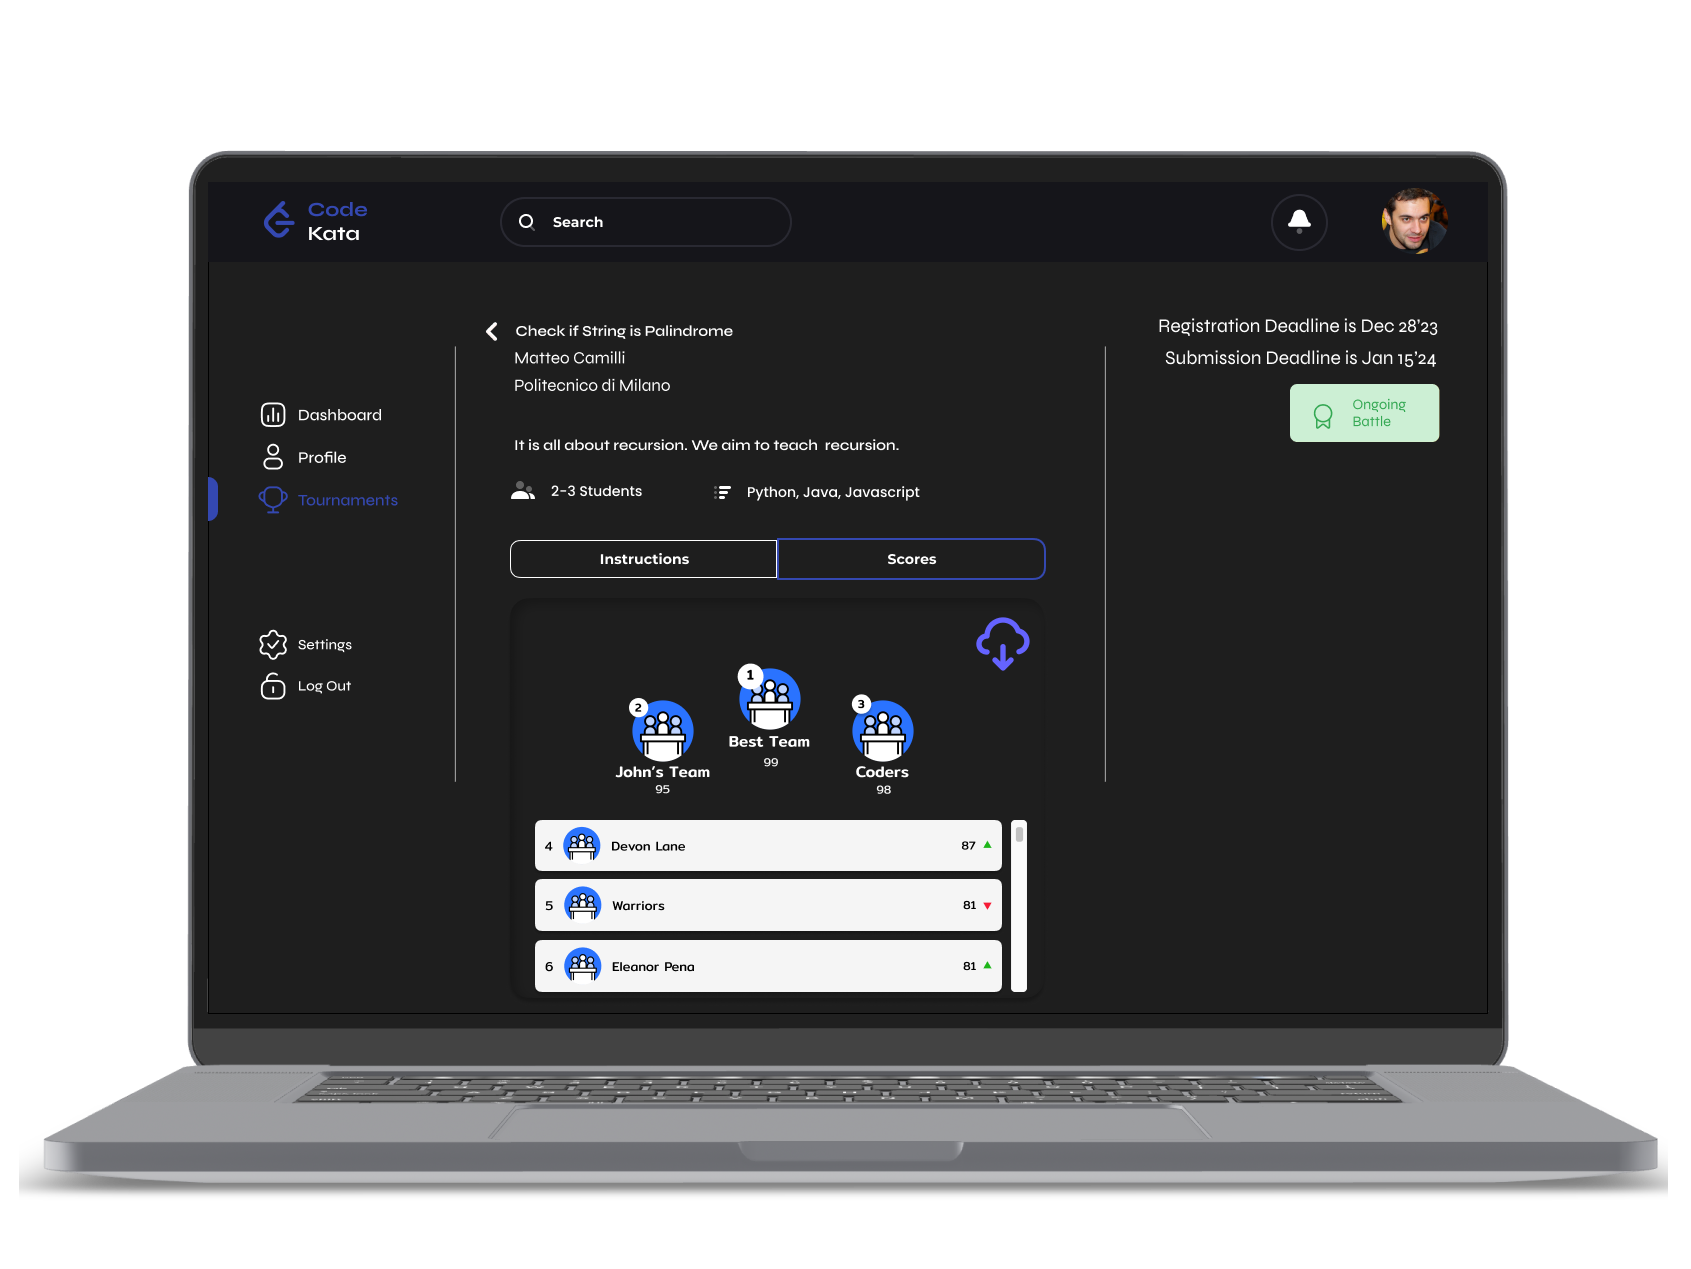
\includegraphics[scale=0.13]{Images/ui-ux/educator_battle/educator_battle_2.png}
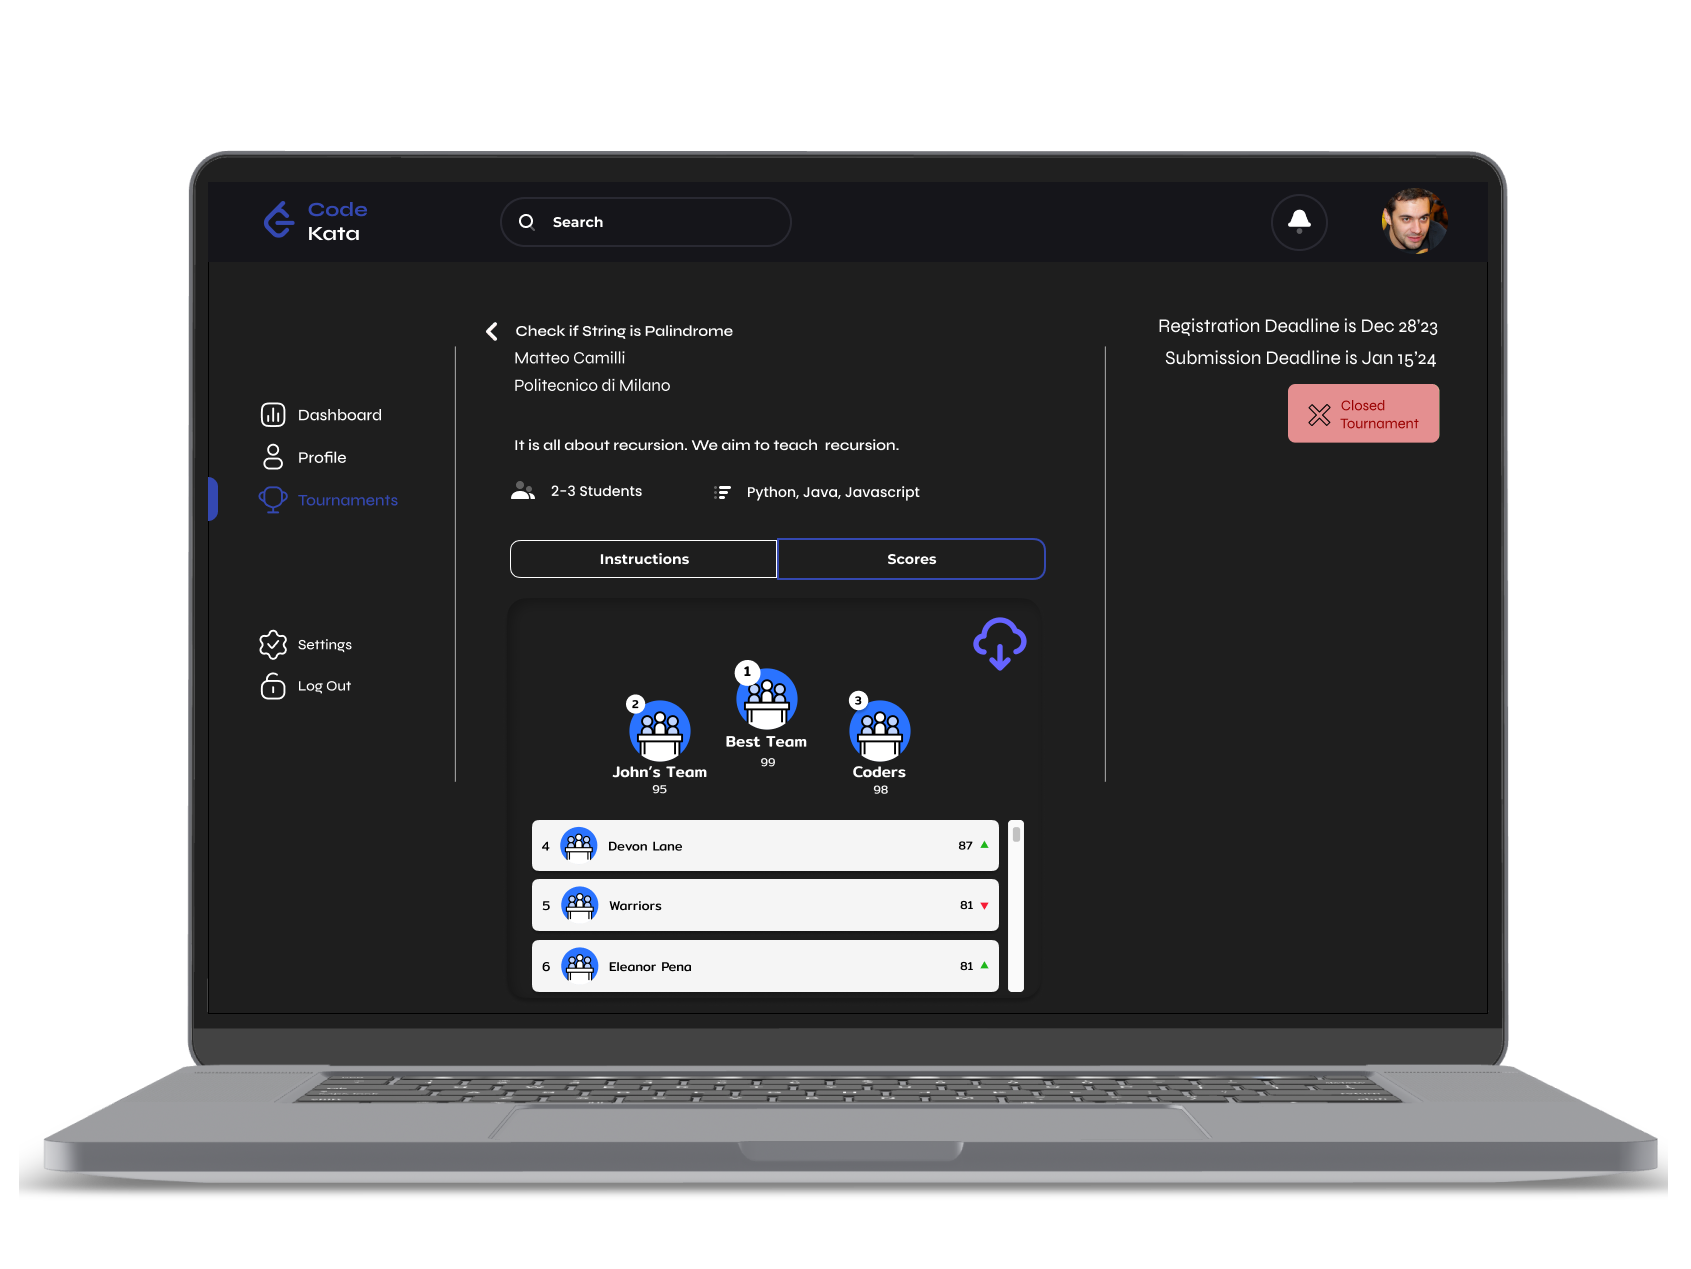
\includegraphics[scale=0.13]{Images/ui-ux/educator_battle/educator_battle_3.png}
\\ (m) Educator visits Battle
\end{center}
\newpage
\begin{center}
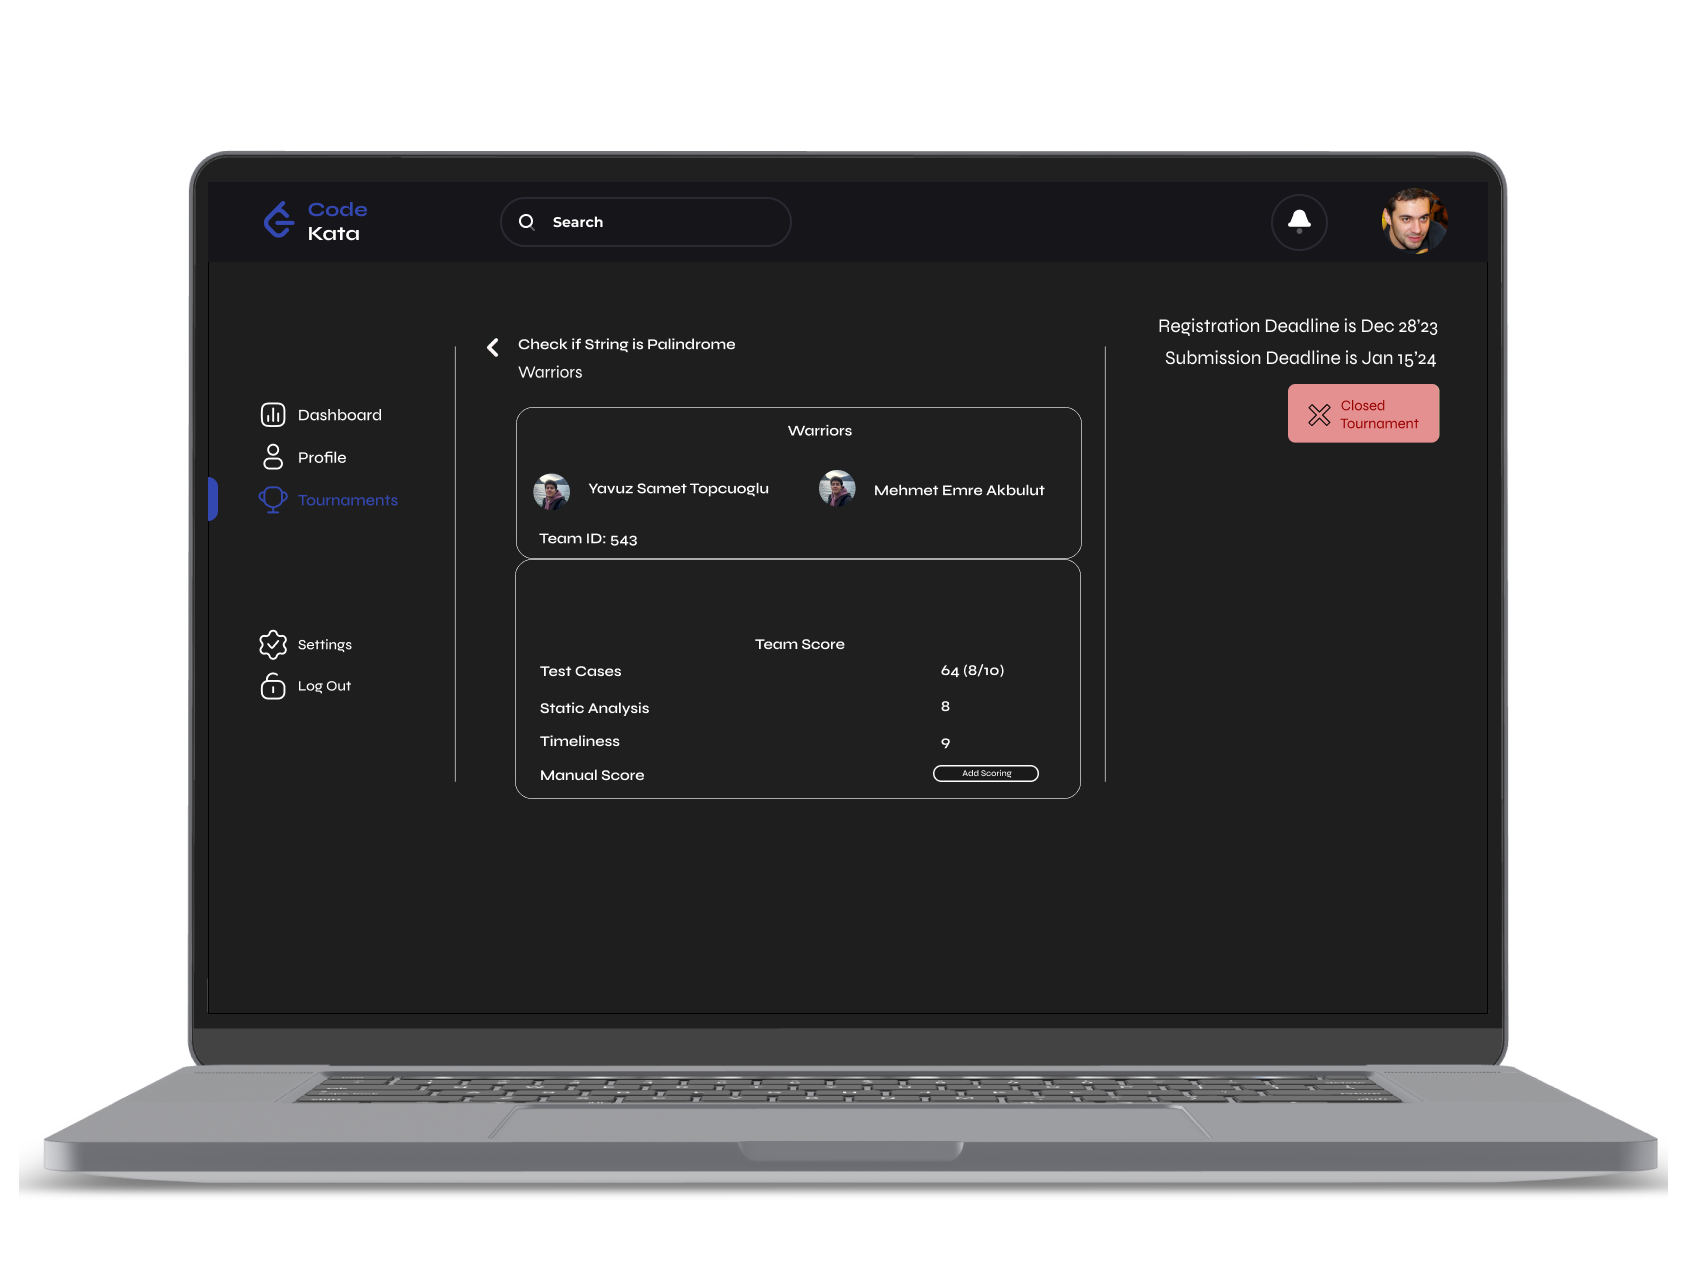
\includegraphics[scale=0.13]{Images/ui-ux/educator_team/educator_team_1.png}
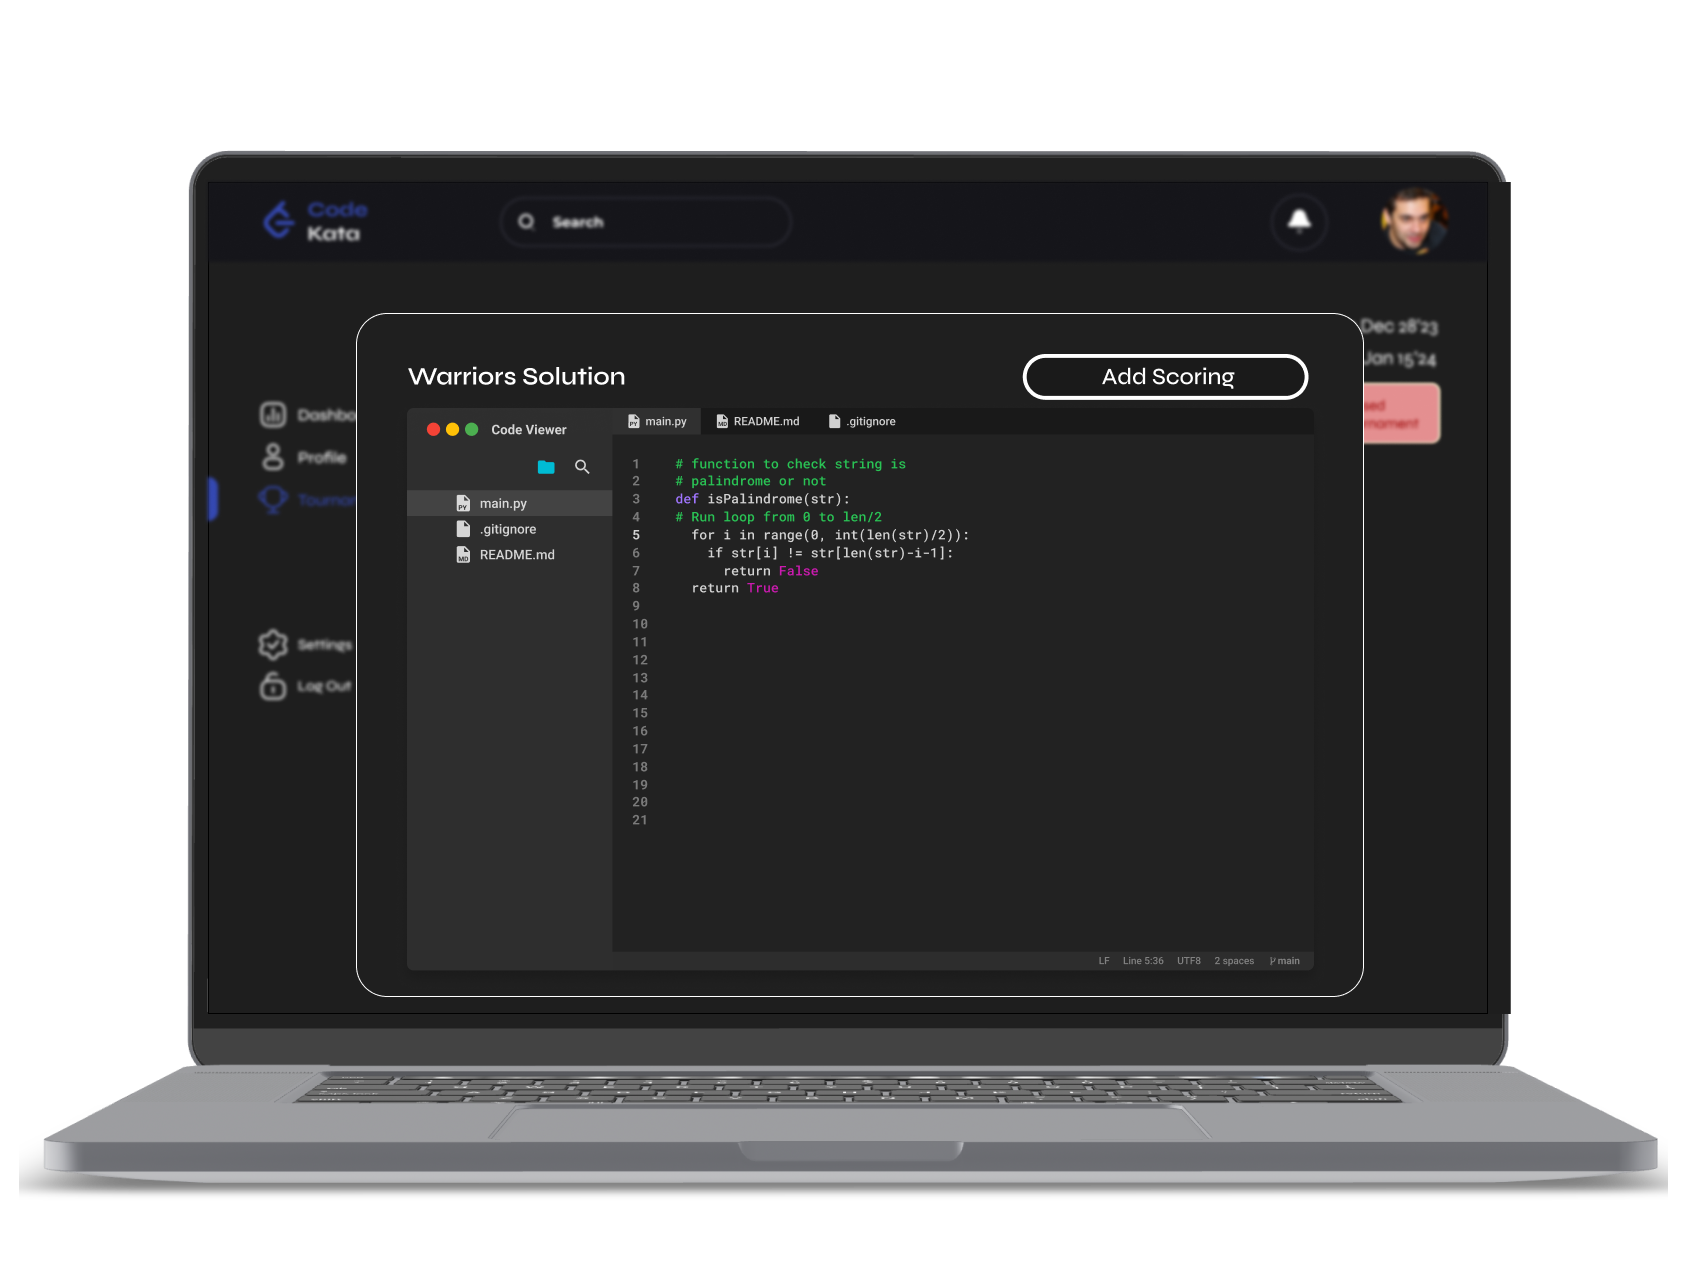
\includegraphics[scale=0.13]{Images/ui-ux/educator_team/educator_team_2.png}
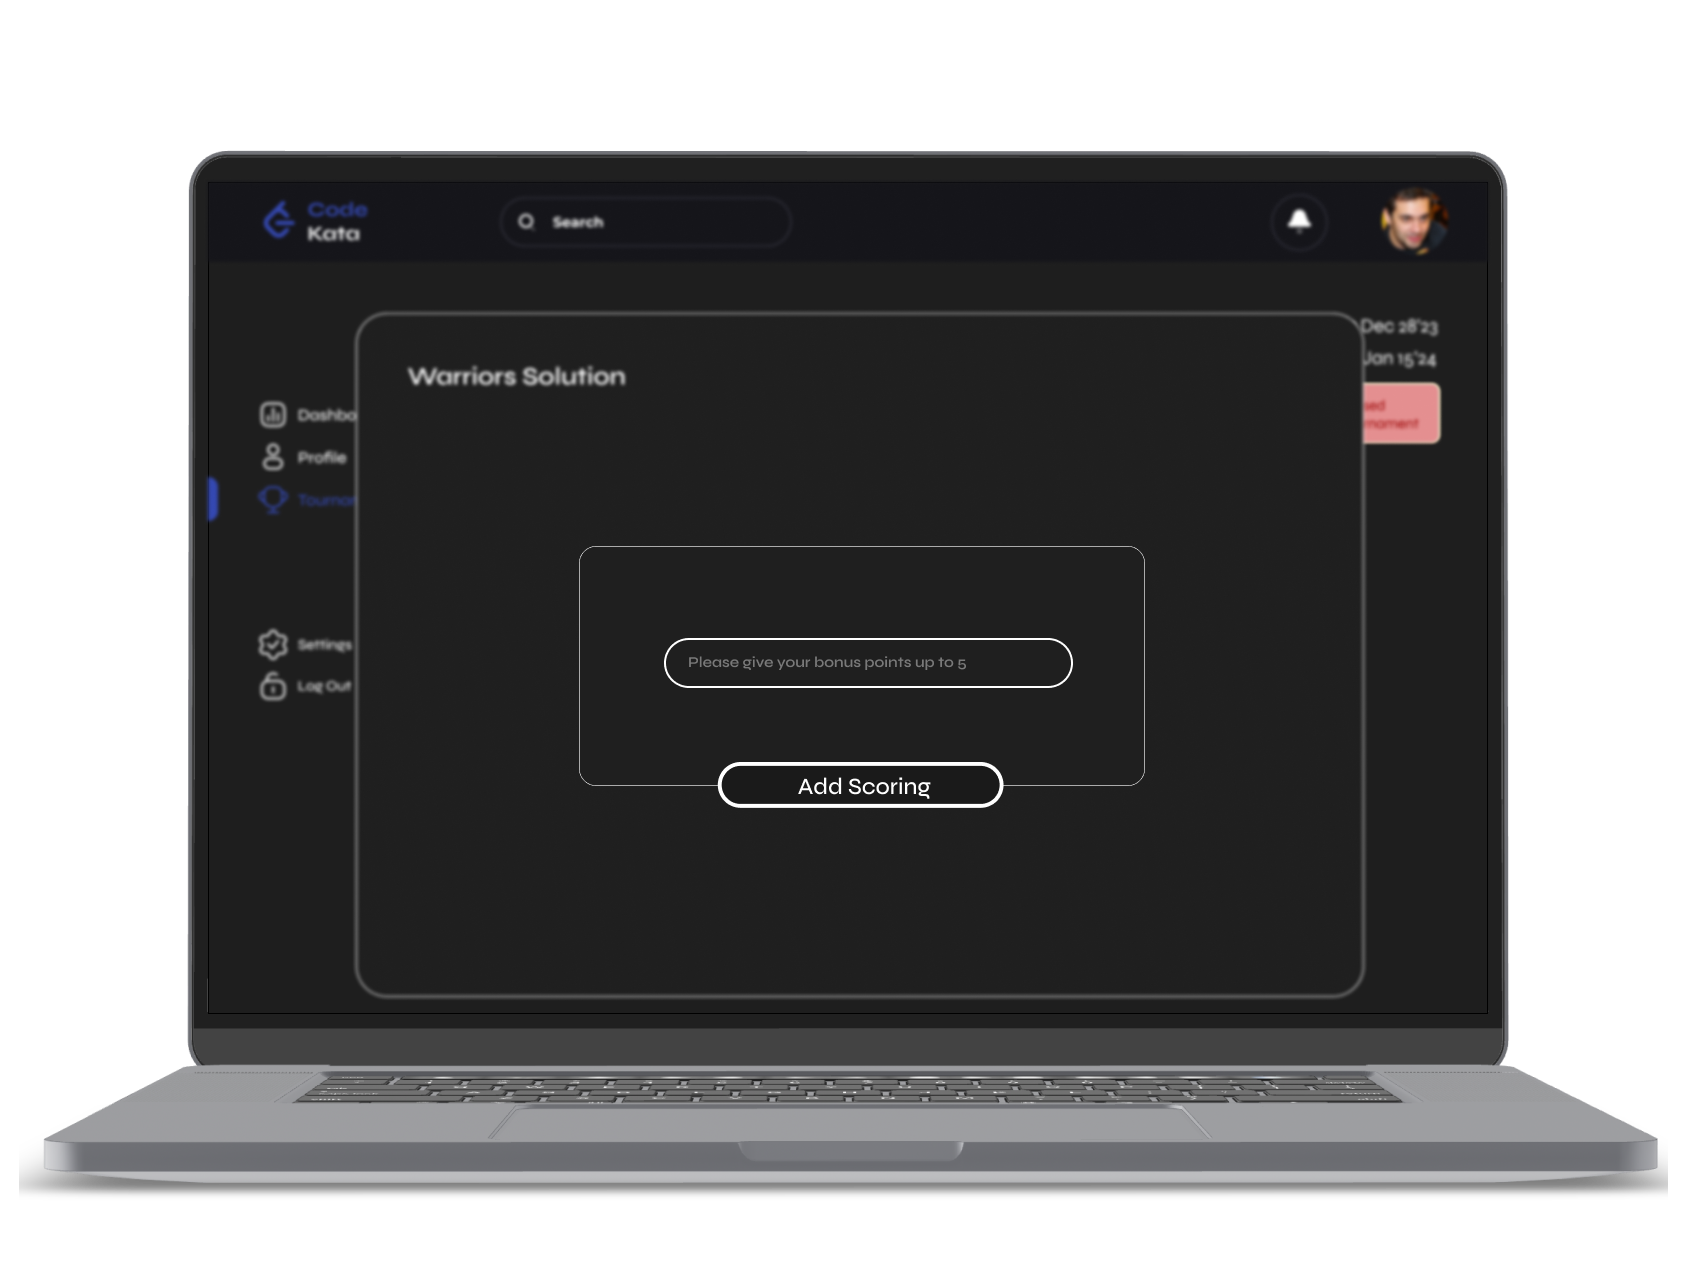
\includegraphics[scale=0.13]{Images/ui-ux/educator_team/educator_team_3.png}
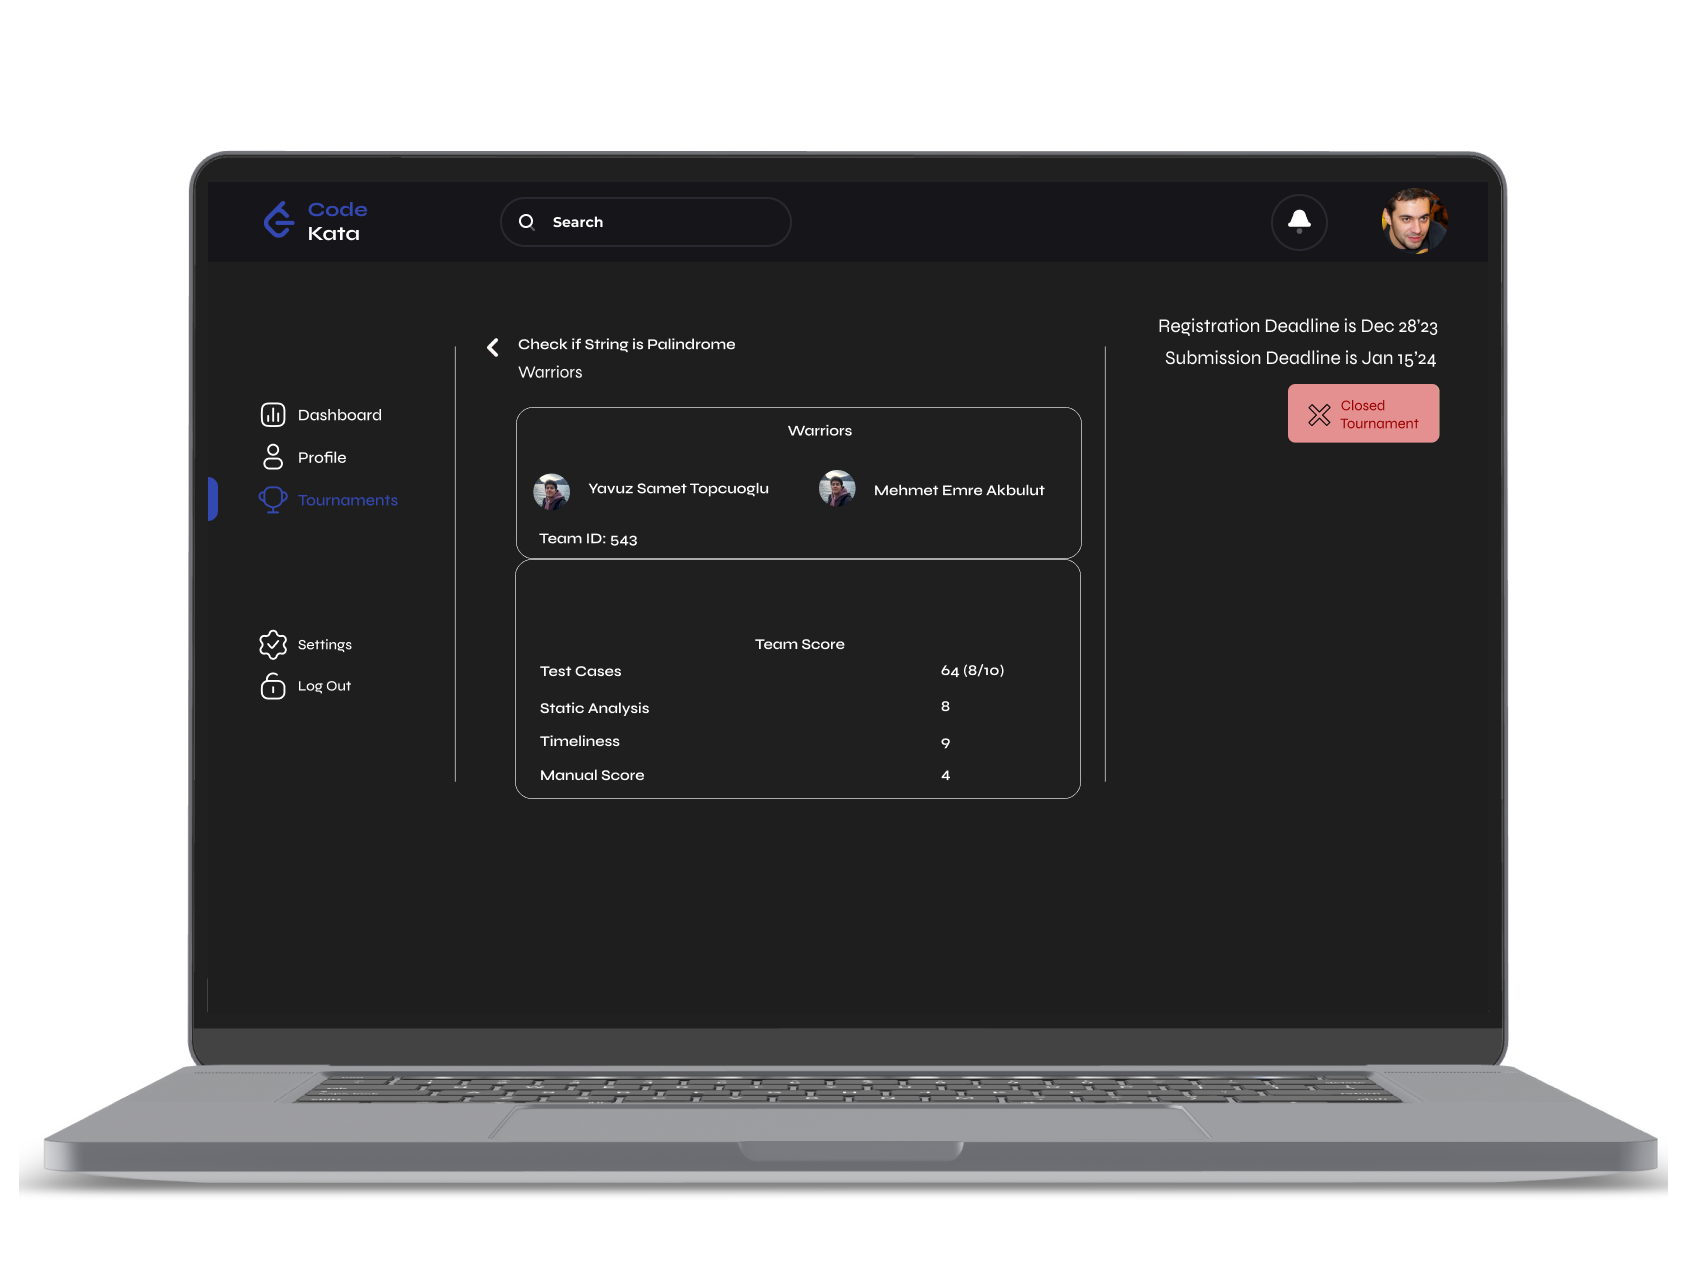
\includegraphics[scale=0.13]{Images/ui-ux/educator_team/educator_team_4.png}
        (n) Educator, Team and Manual Scoring
\end{center}
\begin{center}
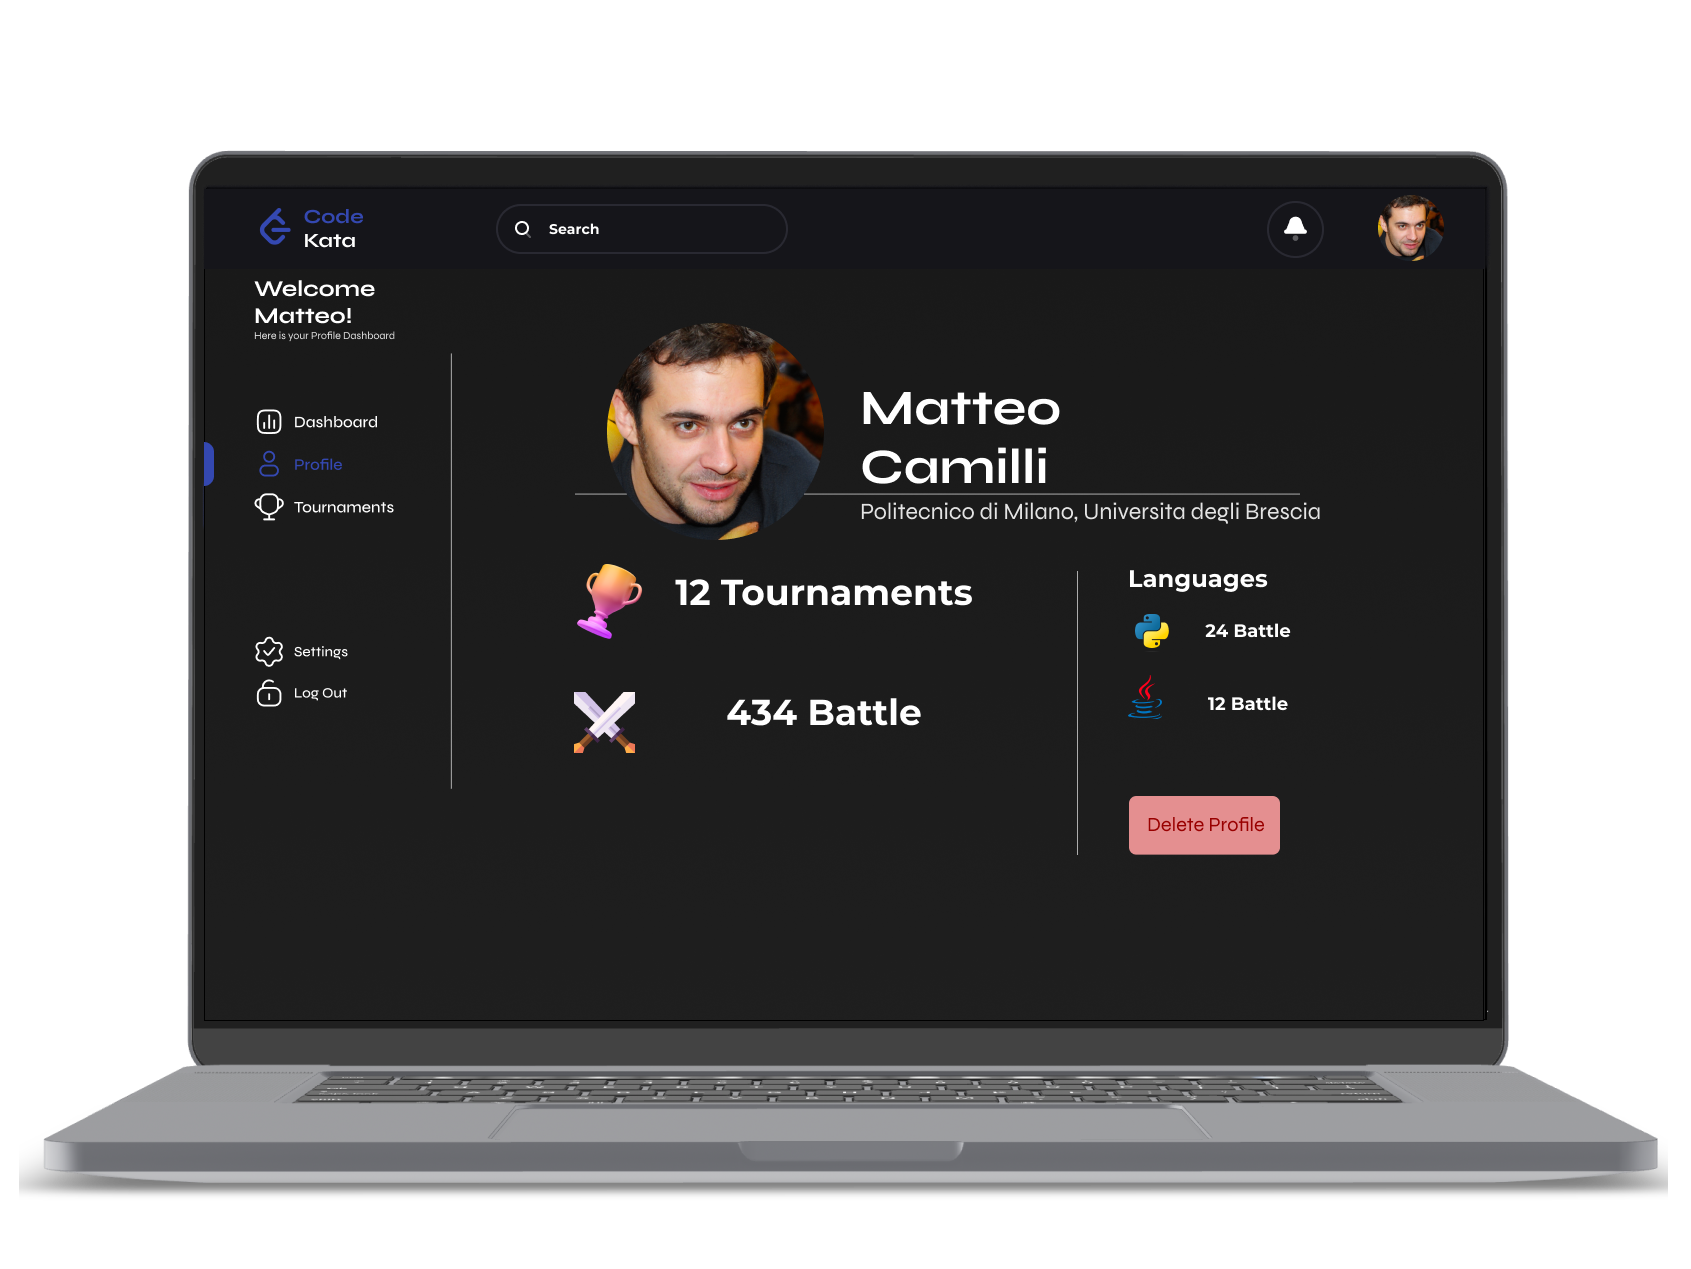
\includegraphics[scale=0.13]{Images/ui-ux/educator_profile_settings/educator_profile.png}
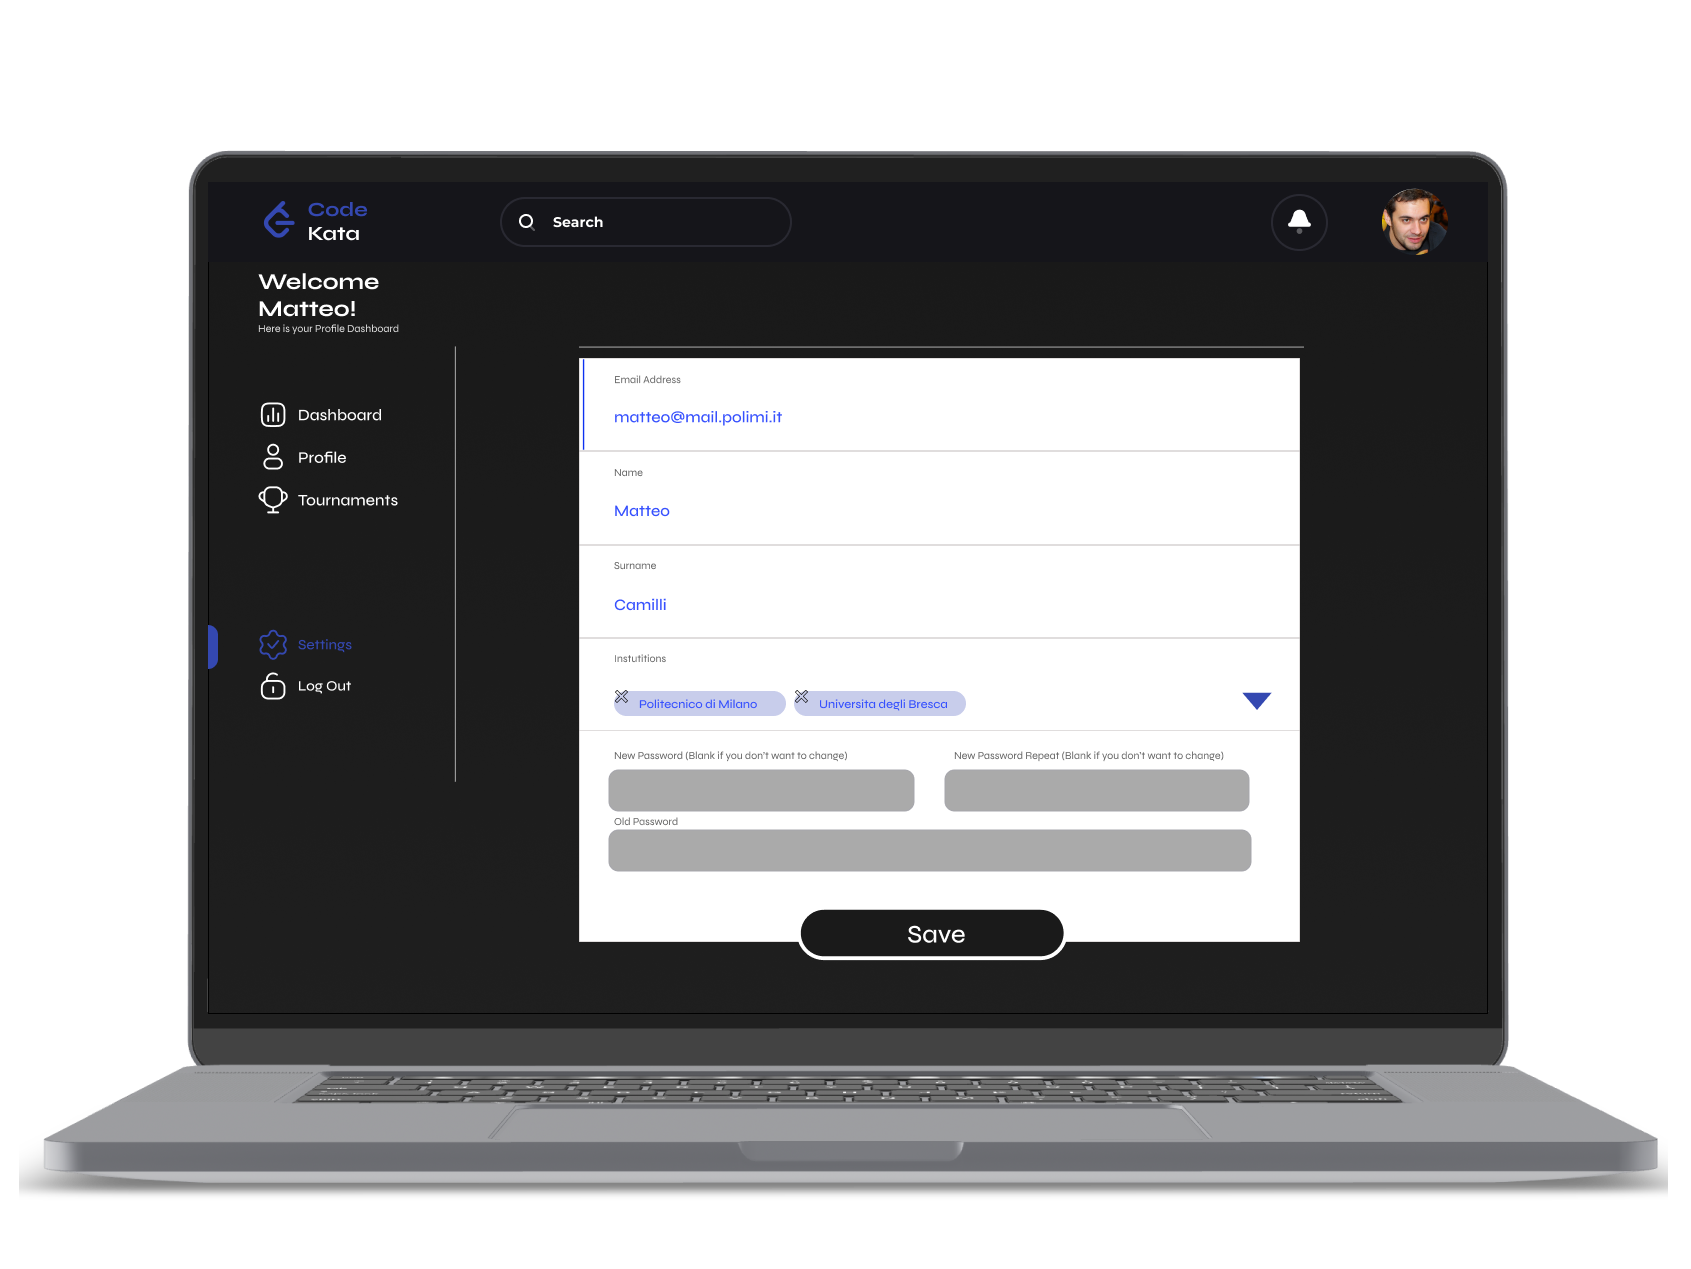
\includegraphics[scale=0.13]{Images/ui-ux/educator_profile_settings/educator_settings.png}
        (o) Educator Profile and Settings
\end{center}
\newpage
\begin{center}
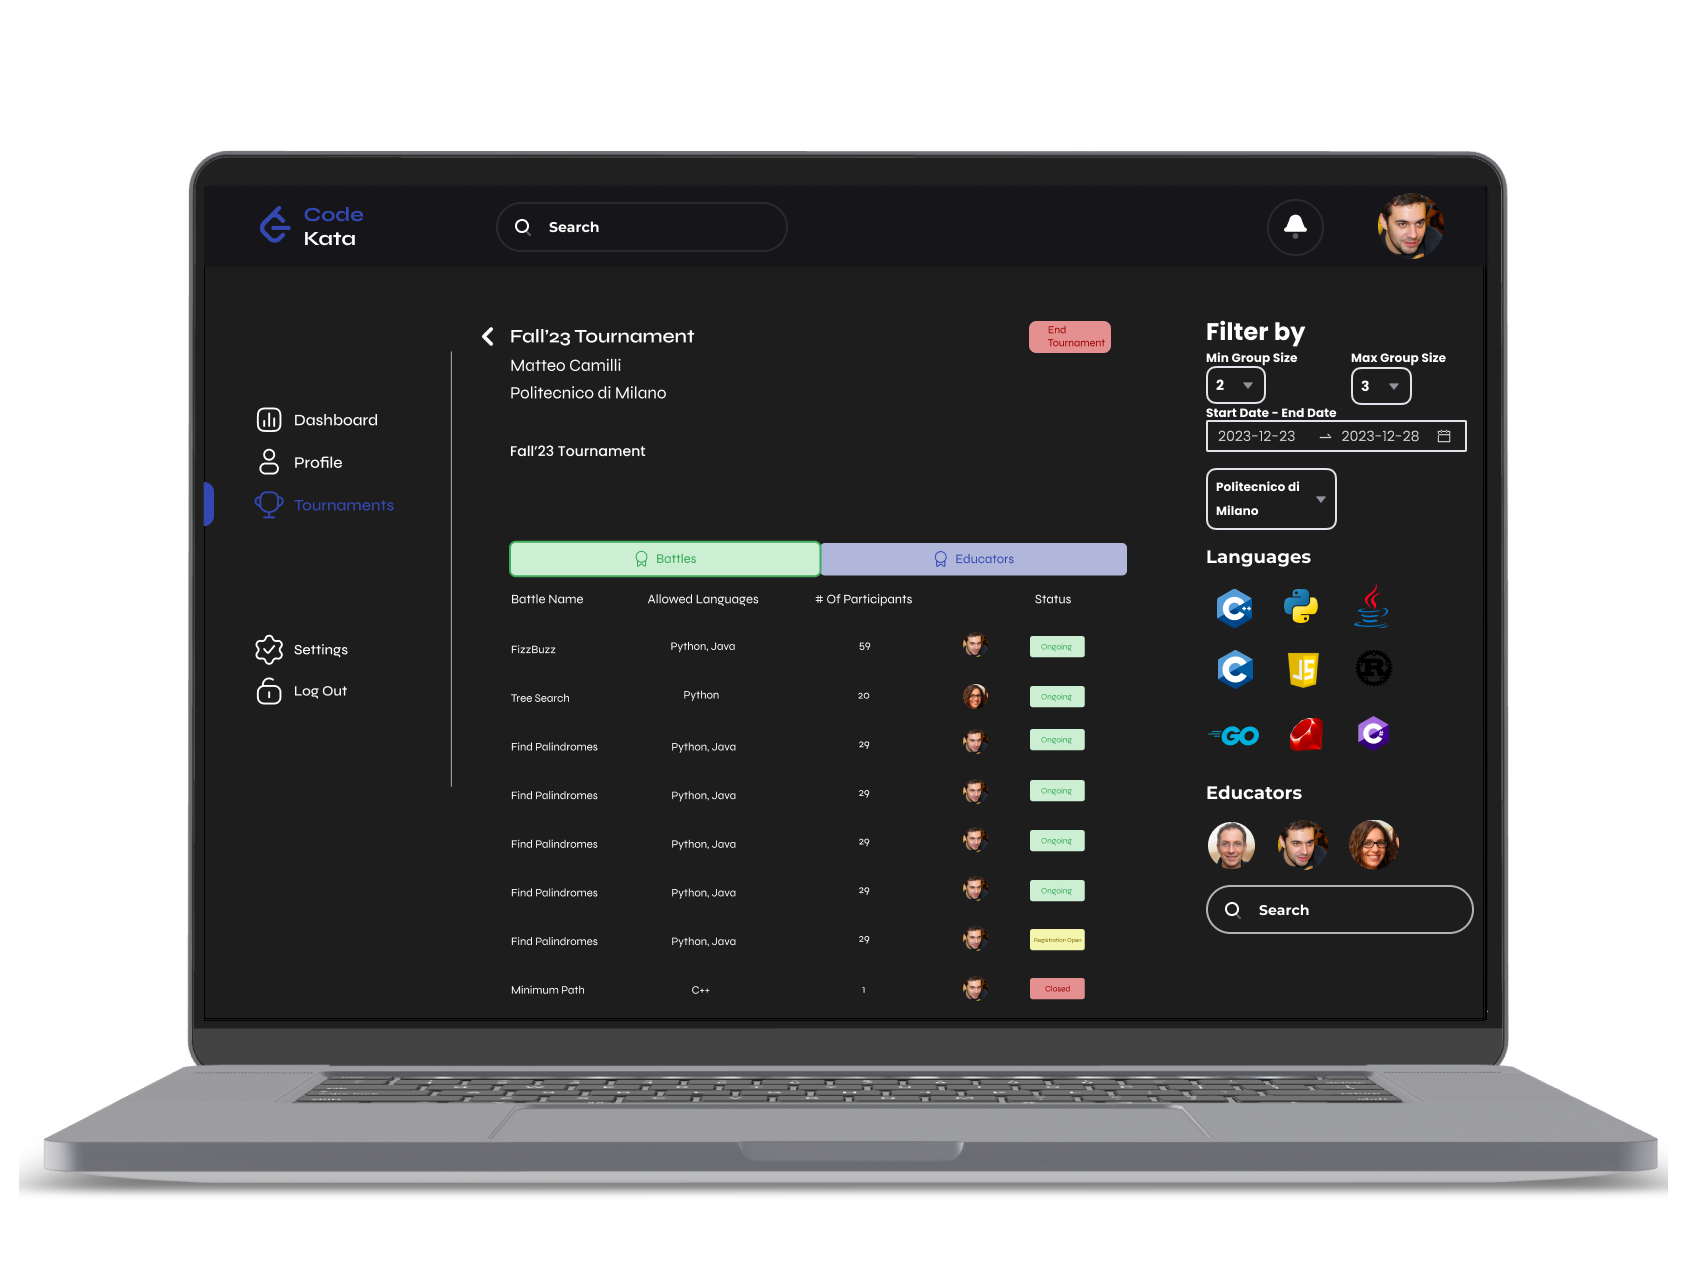
\includegraphics[scale=0.13]{Images/ui-ux/educator_end_tournament/educator_end_tournament.png}
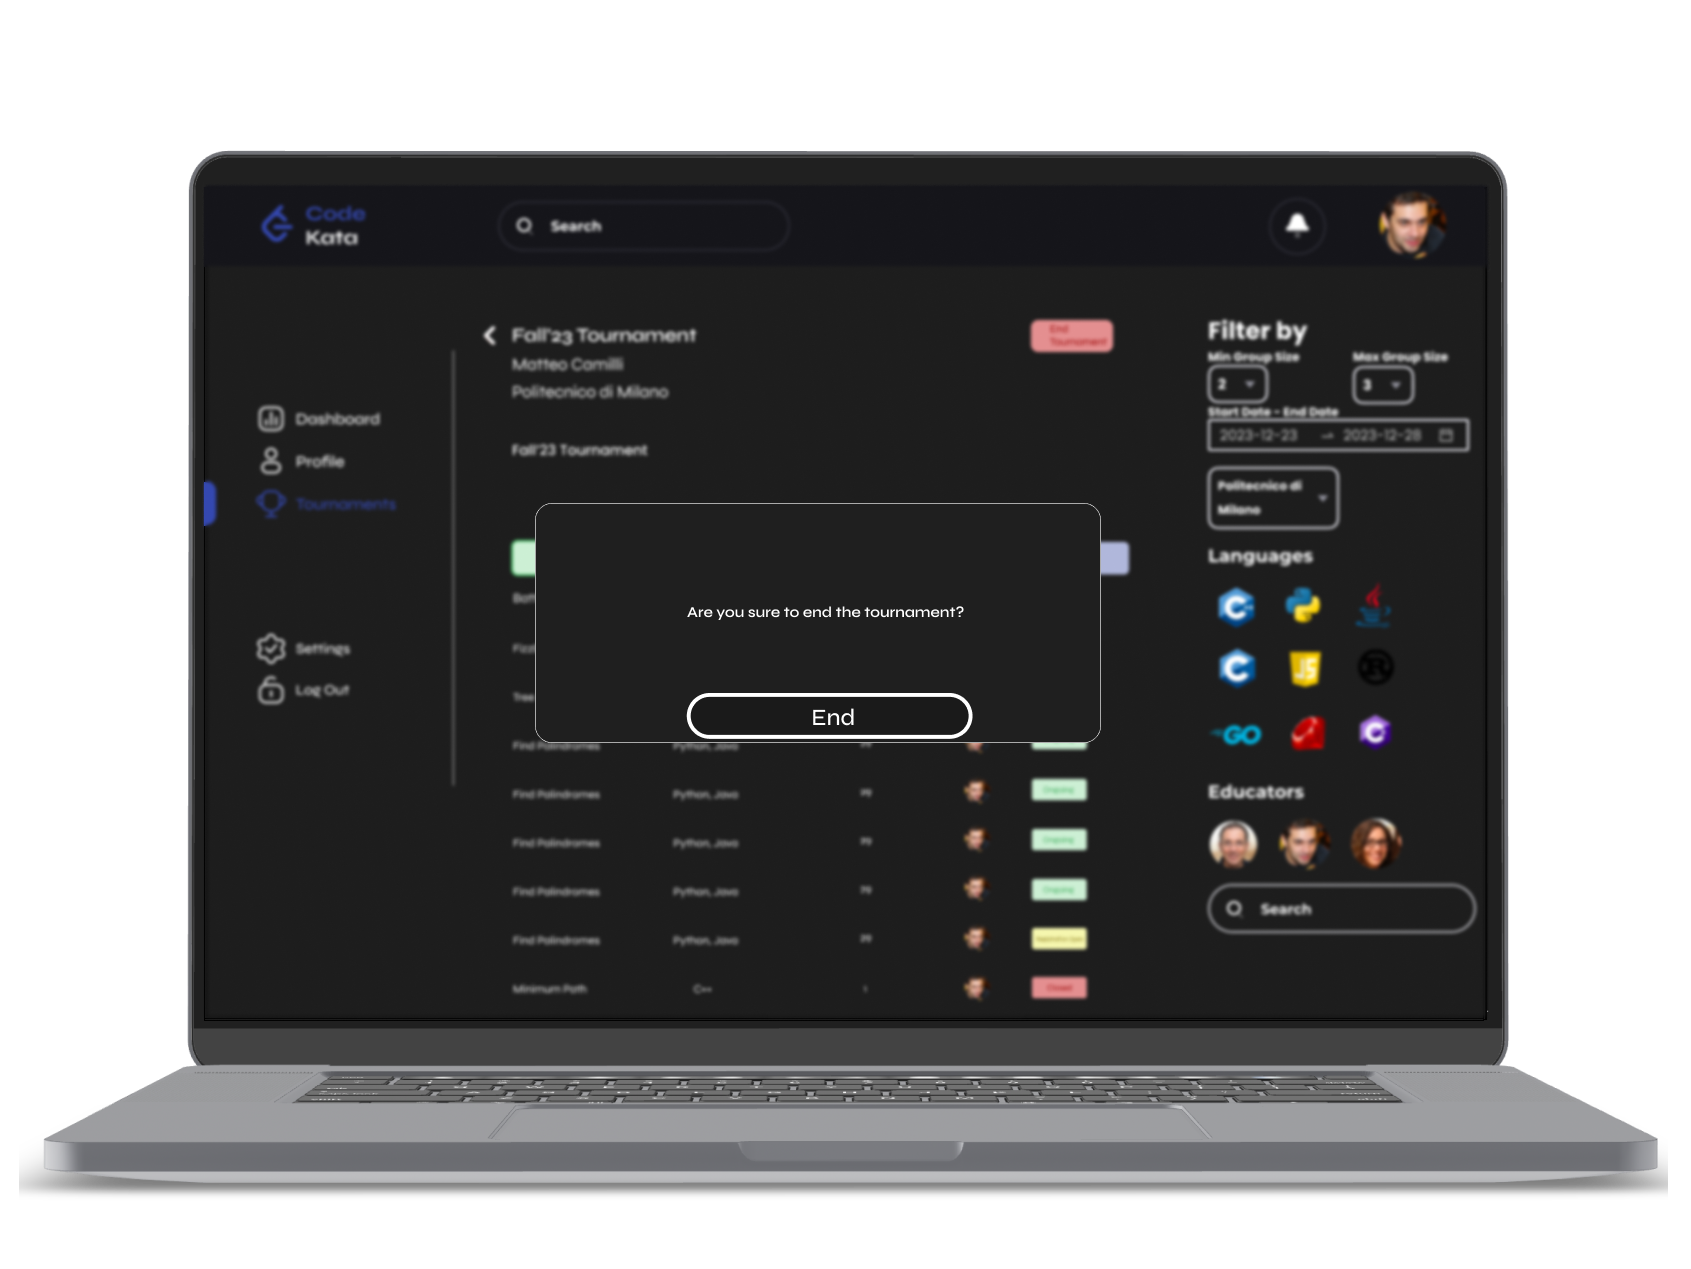
\includegraphics[scale=0.13]{Images/ui-ux/educator_end_tournament/educator_end_tournament_1.png}
        (p) Educator Ends Tournament
\end{center}
\newpage
    
\subsubsection{Hardware Interfaces}
The CodeKataBattle platform operates entirely through web interfaces, eliminating the need for specialized hardware interfaces. Users can access the platform using standard web-enabled devices, such as computers, tablets, and smartphones. The platform is designed to function within a web browser, requiring no specific hardware beyond a device capable of running a modern browser and accessing the internet. This approach ensures broad accessibility without necessitating particular hardware configurations, making the platform versatile and user-friendly across various hardware setups. However, for optimal experience, at least 2GB of RAM and a minimum of 1GB of free space are recommended for browser caching and temporary files.

\subsubsection{Software Interfaces}
Our platform CKB interfaces with various software systems:

\begin{itemize}
    \item \textbf{Web Browsers:} Platform operates on web browsers. For universal access and easy use, it is compatible with major browsers like Chrome, Edge, Safari, Opera, and Firefox.

    \item \textbf{GitHub API:} Integrated for creating coding repositories and managing code \textit{submission} processes.

    \item \textbf{Sandboxing:} To create an isolated testing environment, this approach helps to create a reliable running environment while calculating test case scores.

    \item \textbf{Static Analysis Tool:} An external API will be integrated for scoring the quality aspect of the code with static analysis. 

    \item \textbf{Database Technology:} The data in the platform is consistent and needs to be stored in a database.

    \item \textbf{Hosting:} Our platform needs a web service that provides secure, resizable compute capacity in the cloud for web server and database hosting.

    \item \textbf{Cloud File Storage:} The files will be stored using object storage through a web service interface deployed in the cloud.
    \item \textbf{Email Service:} A simple Email Service will be used to send automated email notifications.
\end{itemize}

\subsubsection{Communication Interfaces}
Our platform utilises various communication systems:

\begin{itemize}
    \item \textbf{HTTPS:} For secure connection over the internet.

    \item \textbf{RESTful APIs:} We have RESTful APIs to communicate with the requests coming from GitHub Actions and the web application.

    \item \textbf{SMTP:} It is used to manage to send automated emails.
\end{itemize}


\subsection{Functional Requirements}
\subsubsection{Use Case Diagram}
\label{sec:Use Case Diagram}

\begin{figure}[H]
    \centering
    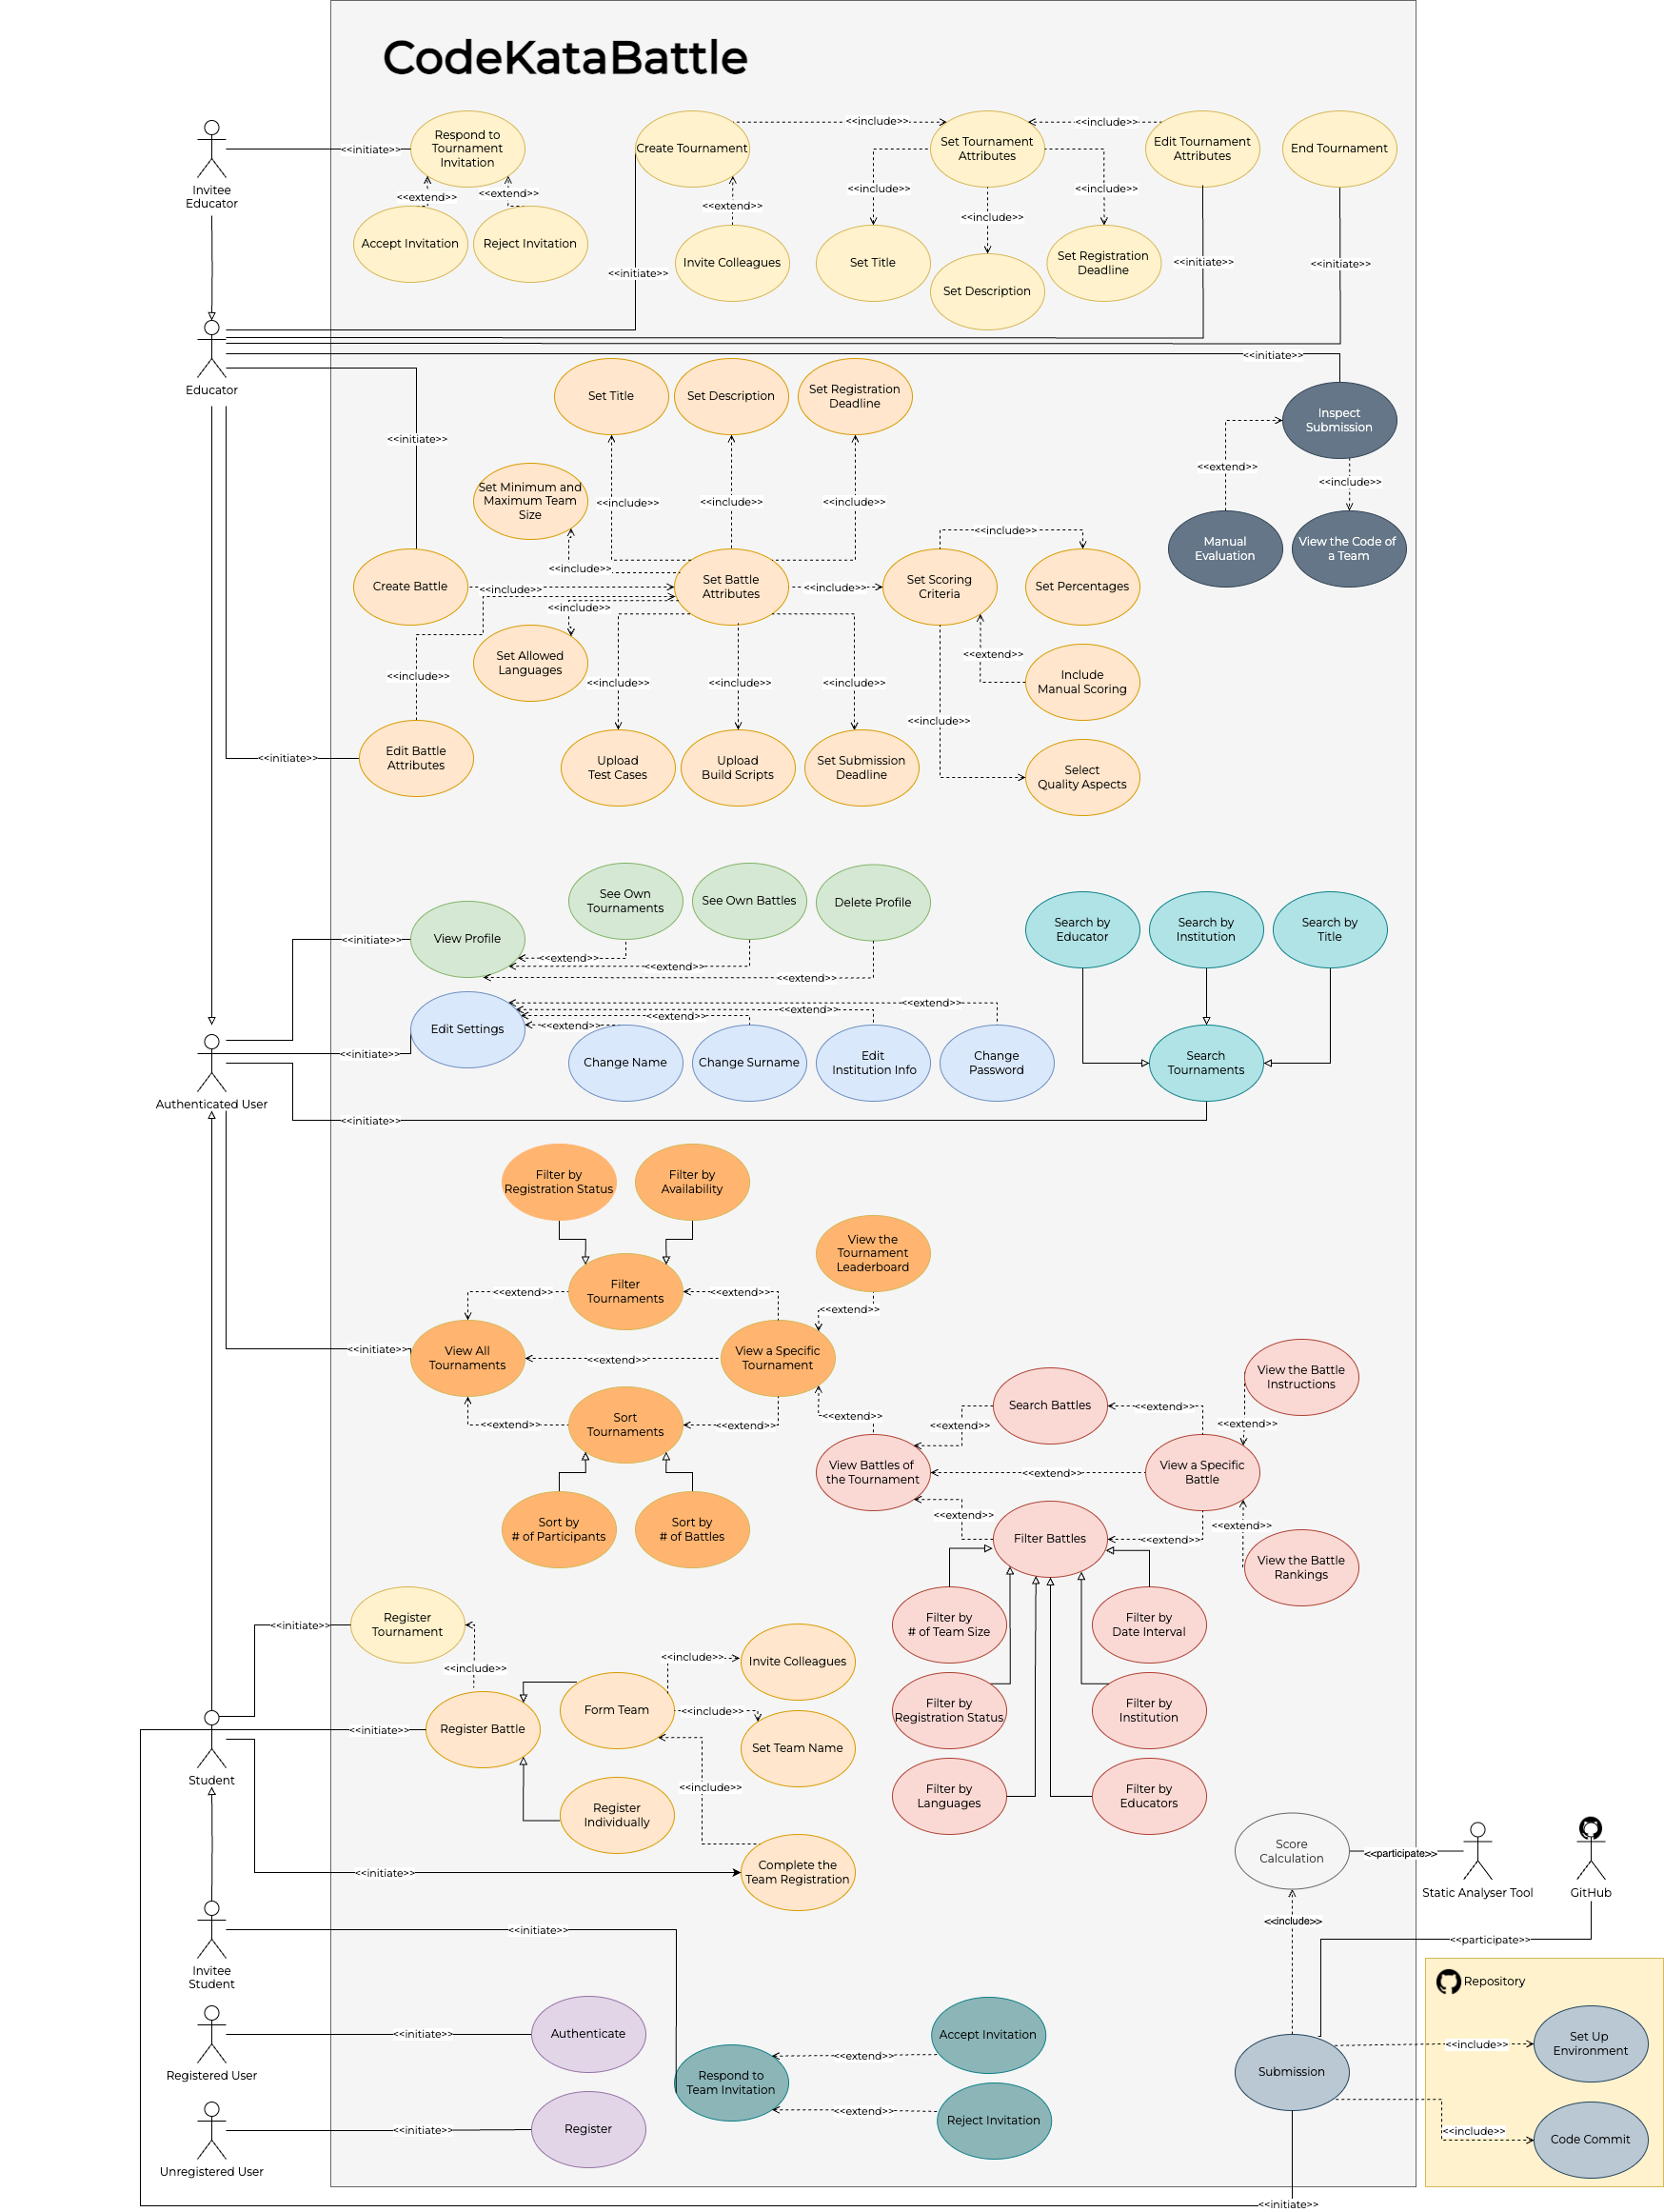
\includegraphics[scale=0.25]{Images/usecasefinal.drawio.png}
    \caption{Use Case Diagram}
\end{figure}


Unregistered User Actor has been used to illustrate the Registration Use Case. Similarly, the Registered User Actor has been used to show the Authentication Use Case. Other user actors are assumed to be registered and authenticated.

\\

Our system is composed of two main user types: Student and Educator. In the use case diagram, we showed common use cases with the Authenticated User actor. Authenticated User, simply every user registered to the platform, can view Tournaments, Battles, and their rankings with different filters and search options. Moreover, Registered User has the capability of viewing their profile and editing settings.

\\

Use case related Educator and Student Actors summarizes the goal of these users in the system.

\\

Invitee Student and Invitee Educator Actors are used to demonstrate use cases for tournament (for educators) and team (for students) invitations.

\\

GitHub System Boundary contains use cases about code submission with the participation of GitHub API Actor.

\subsubsection{Use Cases}

The Use Case Tables below, depict the possible use cases in detail. We tried to cover all the use cases that are included in the Use Case Diagram (see \hyperref[sec:Use Case Diagram]{3.2.1}). However, to reduce the complexity and the number of tables, some use cases that are strongly related to each other have been introduced in the same use case table. To keep track of them, they are written in \textit{italic} in the Event Flow if they occur. Additionally, the Related Use Case(s) row is added to the tables, to see explicitly which use cases from the Use Case Diagram are included in the table. 

\newpage
\begin{enumerate}
    \item Register
    \begin{center}
        \begin{tabular}{ | m{10em} | m{10cm}| } 
          \hline
          \textbf{Name} & Register  \\ 
          \hline
         \textbf{Actor(s)} & Unregistered User \\ 
          \hline
          \textbf{Entry Condition} & The user is unregistered to the platform. \\ 
          \hline
          \textbf{Event Flow} & 
          \begin{enumerate}[(1)]
              \item The actor enters the platform and clicks the Sign Up button.
              \item The actor fills out the registration form by providing email, password, name, surname, and institution information.
              \item The actor clicks the Sign Up button to \textit{register}.
          \end{enumerate} \\
          \hline
          \textbf{Exit Condition} & The actor is registered and the Login page is displayed.  \\ 
          \hline
          \textbf{Related Use Case(s)} & 
            \begin{itemize}
                \item \textit{Register}
            \end{itemize}  \\ 
          \hline
        \end{tabular}
        \captionof{table}{$UC_{1}$ - Register}\label{tbl:uc1}
    \end{center}

 
    
    \item Login
    \begin{center}
    \begin{tabular}{ | m{10em} | m{10cm}| } 
      \hline
      \textbf{Name} & Login (i.e. Authenticate)  \\ 
      \hline
      \textbf{Actor(s)} & Registered User \\ 
      \hline
      \textbf{Entry Condition} & The user is already registered to the platform. \\ 
      \hline
      \textbf{Event Flow} & 
          \begin{enumerate}[(1)]
              \item The actor enters the platform web page.
              \item The actor fills out the form by providing an email address and a password.
              \item The actor clicks the Login button to \textit{authenticate}.
          \end{enumerate}
      \\ 
      \hline
      \textbf{Exit Condition} & The actor is logged in and the dashboard is displayed.  \\ 
      \hline
      \textbf{Exception(s)} & 
      \begin{itemize}
          \item The email and password do not match.
      \end{itemize}
      \\ 
      \hline
      \textbf{Related Use Case(s)} & 
      \begin{itemize}
          \item \textit{Authenticate}
      \end{itemize}
      \\
      \hline
    \end{tabular}
            \captionof{table}{$UC_{2}$ - Login}\label{tbl:uc2}
\end{center}
\newpage
\item View a Tournament
    \begin{center}
    \begin{tabular}{ | m{10em} | m{10cm}| } 
      \hline
      \textbf{Name} & View a Tournament  \\ 
      \hline
      \textbf{Actor(s)} & Authenticated User \\ 
      \hline
      \textbf{Entry Condition} & The actor is logged in. \\ 
      \hline
      \textbf{Event Flow} & 
          \begin{enumerate}[(1)]
              \item The actor clicks the Tournaments button from the sidebar.
              \item In the tournaments page, the actor \textit{views all tournaments} as cards.
              \item The actor \textit{filters tournaments} by registered filter.
              \item The actor \textit{sorts tournaments} by \# of participants.
              \item The actor clicks the first tournament card to \textit{view a specific tournament}.
          \end{enumerate}
      \\ 
      \hline
      \textbf{Exit Condition} & The specific tournament that the actor wants to view is displayed.  \\ 
      \hline
      \textbf{Exception(s)} & 
      \begin{itemize}
          \item There are no existing tournaments.
          \item There are no tournaments with the filter set by the actor.
      \end{itemize}
          \\ 
      \hline
      \textbf{Related Use Case(s)} & 
      \begin{itemize}
          \item \textit{View All Tournaments}
          \item \textit{Filter Tournaments}
          \begin{itemize}
              \item \textit{Filter by Registration Status}
          \end{itemize}
          \item \textit{Sort Tournaments}
          \begin{itemize}
            \item \textit{Sort by \# of Participants}
          \end{itemize}
          \item \textit{View a Specific Tournament}
      \end{itemize}
          \\ 
      \hline
    \end{tabular}
            \captionof{table}{$UC_{3}$ - View Tournament}\label{tbl:uc3}
\end{center}

\newpage

\item View the Tournament Leaderboard
\begin{center}
    \begin{tabular}{ | m{10em} | m{10cm}| } 
      \hline
      \textbf{Name} & View the Tournament Leaderboard \\ 
      \hline
      \textbf{Actor(s)} & Authenticated User \\ 
      \hline
      \textbf{Entry Condition} & The actor is viewing a specific tournament. \\ 
      \hline
      \textbf{Event Flow} & 
          \begin{enumerate}[(1)]
              \item The actor clicks the Leaderboard button to \textit{view the tournament leaderboard}.
          \end{enumerate}
      \\ 
      \hline
      \textbf{Exit Condition} & The leaderboard of that tournament is displayed.  \\ 
      \hline
      \textbf{Related Use Case(s)} & 
      \begin{itemize}
      \item \textit{View the Tournament Leaderboard}
      \end{itemize}
          \\ 
      \hline
    \end{tabular}
    \captionof{table}{$UC_{4}$ - View Tournament Leaderboard}\label{tbl:uc4}
\end{center}


\item View a Battle
    \begin{center}
    \begin{tabular}{ | m{10em} | m{10cm}| } 
      \hline
      \textbf{Name} & View a Battle  \\ 
      \hline
      \textbf{Actor(s)} & Authenticated User \\ 
      \hline
      \textbf{Entry Condition} & The actor is viewing a specific tournament. \\ 
      \hline
      \textbf{Event Flow} & 
          \begin{enumerate}[(1)]
              \item The actor \textit{views the battles of the tournament} in that tournament's page.
              \item The actor \textit{searches battles} using the search bar at the bottom of the page.
              \item The actor \textit{filters battles} using the filter section on the right-hand side of the page.
              \item The actor chooses one of the results to \textit{view a specific battle}.
          \end{enumerate}
      \\ 
      \hline
      \textbf{Exit Condition} & The specific battle that the actor wants to view is displayed.  \\ 
      \hline
      \textbf{Exception(s)} & 
      \begin{itemize}
          \item There are no existing battles in that tournament.
          \item There are no battles with the filters set by the actor.
      \end{itemize}
          \\ 
      \hline
      \textbf{Related Use Case(s)} & 
      \begin{itemize}
          \item \textit{View Battles of the Tournament}
          \item \textit{Search Battles}
          \item \textit{Filter Battles}
          \item \textit{View a Specific Battle}
      \end{itemize}
          \\ 
      \hline
    \end{tabular}
    \captionof{table}{$UC_{5}$ - View Battle}\label{tbl:uc5}
\end{center}


\newpage


\item View the Battle Instructions
\begin{center}
    \begin{tabular}{ | m{10em} | m{10cm}| } 
      \hline
      \textbf{Name} & View the Battle Instructions \\ 
      \hline
      \textbf{Actor(s)} & Authenticated User \\ 
      \hline
      \textbf{Entry Condition} & The actor is viewing a specific battle. \\ 
      \hline
      \textbf{Event Flow} & 
          \begin{enumerate}[(1)]
              \item The actor clicks the Instructions button to \textit{view the battle instructions}.
          \end{enumerate}
      \\ 
      \hline
      \textbf{Exit Condition} & The instructions of that battle are displayed.  \\ 
      \hline
      \textbf{Related Use Case(s)} & 
      \begin{itemize}
          \item \textit{View the Battle Instructions}
      \end{itemize}
          \\ 
      \hline
    \end{tabular}
    \captionof{table}{$UC_{6}$ - View Battle Instructions}\label{tbl:uc6}
\end{center}

\item View the Battle Rankings
\begin{center}
    \begin{tabular}{ | m{10em} | m{10cm}| } 
      \hline
      \textbf{Name} & View the Battle Rankings \\ 
      \hline
      \textbf{Actor(s)} & Authenticated User \\ 
      \hline
      \textbf{Entry Condition} & The actor is viewing a specific battle. \\ 
      \hline
      \textbf{Event Flow} & 
          \begin{enumerate}[(1)]
              \item The actor clicks the Scores button to \textit{view the battle rankings}.
          \end{enumerate}
      \\ 
      \hline
      \textbf{Exit Condition} & The rankings of that battle are displayed.  \\ 
      \hline
      \textbf{Related Use Case(s)} & 
      \begin{itemize}
\item \textit{View the Battle Rankings}
      \end{itemize}
          \\ 
      \hline
    \end{tabular}
    \captionof{table}{$UC_{7}$ - View Battle Rankings}\label{tbl:uc7}
\end{center}

\newpage
\item Inspect a Submission
\begin{center}
    \begin{tabular}{ | m{10em} | m{10cm}| } 
      \hline
      \textbf{Name} & Inspect a Submission \\ 
      \hline
      \textbf{Actor(s)} & Educator \\ 
      \hline
      \textbf{Entry Condition} & The actor is viewing the battle rankings of a specific battle. \\ 
      \hline
      \textbf{Event Flow} & 
          \begin{enumerate}[(1)]
              \item The actor clicks one of the teams from the rankings table to \textit{view the team's submission}.
              \item The actor looks at the code and decides to \textit{manually evaluate}.
              \item The actor enters the bonus points in the respective field and clicks the Add Scoring button.
          \end{enumerate}
      \\ 
      \hline
      \textbf{Exit Condition} & The total score after manual evaluation of that team are displayed.  \\ 
      \hline
      \textbf{Exception(s)} & 
      \begin{itemize}
          \item The manual scoring is not enabled.
      \end{itemize}
          \\ 
      \hline
      \textbf{Related Use Case(s)} & 
      \begin{itemize}
\item \textit{View the Code of a Team}
\item \textit{Manual Evaluation}
      \end{itemize}
          \\ 
      \hline
    \end{tabular}
    \captionof{table}{$UC_{8}$ - Inspect Submission}\label{tbl:uc8}
\end{center}


\newpage


\item Search Tournaments
\begin{center}
    \begin{tabular}{ | m{10em} | m{10cm}| } 
      \hline
      \textbf{Name} & Search Tournament  \\ 
      \hline
      \textbf{Actor(s)} & Authenticated User \\ 
      \hline
      \textbf{Entry Condition} & The user is logged in. \\ 
      \hline
      \textbf{Event Flow} & 
          \begin{enumerate}[(1)]
              \item The actor clicks the button in the search area to select the search criteria.
              \item The actor sees three buttons: \textit{Search by Educators}, \textit{Search by Titles}, \textit{Search by Institutions} and chooses to search by title.
              \item The actor writes "Fall'23 Tournament" to the search bar and hits enter to \textit{search tournament}.
          \end{enumerate}
      \\ 
      \hline
      \textbf{Exit Condition} & The tournaments with the corresponding title are displayed.  \\ 
      \hline
      \textbf{Exception(s)} & 
      \begin{itemize}
          \item The tournament with the given title does not exist.
      \end{itemize}
          \\ 
      \hline
      \textbf{Related Use Case(s)} & 
      \begin{itemize}
          \item \textit{Search by Educator}
          \item \textit{Search by Title}
          \item \textit{Search by Institution}
          \item \textit{Search Tournament}
      \end{itemize}
          \\ 
      \hline
    \end{tabular}
        \captionof{table}{$UC_{9}$ - Search Tournaments}\label{tbl:uc9}
\end{center}


\item Register to a Tournament
\begin{center}
    \begin{tabular}{ | m{10em} | m{10cm}| } 
      \hline
      \textbf{Name} & Register to a Tournament  \\ 
      \hline
      \textbf{Actor(s)} & Student \\ 
      \hline
      \textbf{Entry Condition} & The actor is logged in and the tournaments page is on display.\\ 
      \hline
      \textbf{Event Flow} & 
          \begin{enumerate}[(1)]
              \item The actor clicks a card of a tournament in which s/he is not registered.
              \item The actor clicks the Register button in the pop-up to \textit{register the tournament}.
          \end{enumerate}
      \\ 
      \hline
      \textbf{Exit Condition} & The actor is registered to the tournament and the page of that tournament is displayed.  \\ 
      \hline
      \textbf{Exception(s)} & 
      \begin{itemize}
          \item There are not any tournaments with not registered status.
      \end{itemize}
          \\ 
      \hline
      \textbf{Related Use Case(s)} & 
      \begin{itemize}
          \item \textit{Register Tournament}
      \end{itemize}
          \\ 
      \hline
    \end{tabular}
    \captionof{table}{$UC_{10}$ - Register to a Tournament}\label{tbl:uc10}
\end{center}


\newpage


\item Register to a Battle
\begin{center}
    \begin{tabular}{ | m{10em} | m{10cm}| } 
      \hline
      \textbf{Name} & Register to a Battle  \\ 
      \hline
      \textbf{Actor(s)} & Student \\ 
      \hline
      \textbf{Entry Condition} & The actor registered to the tournament in which the battle takes place and that tournament's page is on display. \\ 
      \hline
      \textbf{Event Flow} & 
          \begin{enumerate}[(1)]
              \item The actor clicks a register button next to the battle that s/he wants to participate in.
              \item The actor clicks the Register button in the pop-up.
              \item The actor chooses between to \textit{form a team} and to \textit{register individually}. 
              \item If there is going to be a team, the actor \textit{sets a team name} and \textit{invites colleagues}.
              \item The actor clicks the Complete button to \textit{register to the battle}.
          \end{enumerate}
      \\ 
      \hline
      \textbf{Exit Condition} & 
      \begin{itemize}
          \item If registered individually, the actor is registered to the battle.
          \item If a team is formed, the invitation requests are sent to the colleagues.
      \end{itemize}
        \\ 
      \hline
      \textbf{Exception(s)} & 
      \begin{itemize}
          \item The actor is already registered for all battles in that tournament.
      \end{itemize}
          \\ 
      \hline
      \textbf{Related Use Case(s)} & 
      \begin{itemize}
          \item \textit{Register Battle}
          \item \textit{Form Team}
          \item \textit{Register Individually}
          \item \textit{Invite Colleagues}
          \item \textit{Set Team Name}
      \end{itemize}
          \\ 
      \hline
    \end{tabular}
        \captionof{table}{$UC_{11}$ - Register to a Battle}\label{tbl:uc11}
\end{center}


\newpage

\item Complete the Team Registration for the Battle
\begin{center}
    \begin{tabular}{ | m{10em} | m{10cm}| } 
      \hline
      \textbf{Name} & Complete the Team Registration for the Battle  \\ 
      \hline
      \textbf{Actor(s)} & Student \\ 
      \hline
      \textbf{Entry Condition} & The specific battle that the actor wants to complete the registration is on display. \\ 
      \hline
      \textbf{Event Flow} & 
          \begin{enumerate}[(1)]
              \item The actor can see which colleague accepted the invitation and which colleague rejected it.
              \item The actor can finalize the team formation if there are enough colleagues on the team by using the Finalize button, or discard the team and battle registration entirely by using the Decline button to \textit{complete the team registration}.
          \end{enumerate}
      \\ 
      \hline
      \textbf{Exit Condition} & 
      \begin{itemize}
          \item If finalized, the team is registered to the battle.
          \item If declined, the team is not registered to the battle and the dashboard is displayed.
      \end{itemize}\\ 
      \hline
      \textbf{Related Use Case(s)} & 
      \begin{itemize}
          \item \textit{Complete the Team Registration}
      \end{itemize}
          \\ 
      \hline
    \end{tabular}
        \captionof{table}{$UC_{12}$ - Complete the Team Registration}\label{tbl:uc12}
\end{center}


\item Respond to the Team Invitation
\begin{center}
    \begin{tabular}{ | m{10em} | m{10cm}| } 
      \hline
      \textbf{Name} & Respond to the Team Invitation  \\ 
      \hline
      \textbf{Actor(s)} & Invitee Student \\ 
      \hline
      \textbf{Entry Condition} & The actor is logged in and invited to a team by another student.  \\ 
      \hline
      \textbf{Event Flow} & 
          \begin{enumerate}[(1)]
              \item The actor opens up the notifications and sees the invitation to join a team formed by another student.
              \item The actor clicks the notification and a pop-up shows up.
              \item The actor can choose to \textit{Accept Invitation} by clicking the Accept button or \textit{Reject Invitation} by clicking the Reject button to \textit{respond to the invitation}.
          \end{enumerate}
      \\ 
      \hline
      \textbf{Exit Condition} & 
      \begin{itemize}
          \item If accepted, the specific battle is displayed.
          \item If rejected, the dashboard is displayed.
      \end{itemize}\\ 
      \hline
      \textbf{Related Use Case(s)} & 
      \begin{itemize}
          \item \textit{Accept Invitation}
          \item \textit{Reject Invitation}
          \item \textit{Respond to Team Invitation}
      \end{itemize}
          \\ 
      \hline
    \end{tabular}
        \captionof{table}{$UC_{13}$ - Respond to the Team Invitation}\label{tbl:uc13}
\end{center}



\newpage

\item Submission
\begin{center}
    \begin{tabular}{ | m{10em} | m{10cm}| } 
      \hline
      \textbf{Name} & Submission  \\ 
      \hline
      \textbf{Actor(s)} & Student, GitHub API, Static Analyser Tool \\ 
      \hline
      \textbf{Entry Condition} & The student actor forked the battle repository, and initiated GitHub Actions on their repository. \\ 
      \hline
      \textbf{Event Flow} & 
          \begin{enumerate}[(1)]
              \item The student actor \textit{sets up the necessary environment}.
              \item The student actor works on the problem and writes code. 
              \item The student actor \textit{commits code} to their repository to \textit{make the submission}.
              \item The GitHub API actor informs the CKB platform to pull the code.
              \item The CKB platform pulls the code from the team's repository.
              \item The platform \textit{calculates the score} of the submission with respect to test cases, timeliness, and quality aspects. 
              \item During the calculation of quality aspects, it uses the API provided by the Static Analyser Tool actor.
          \end{enumerate}
      \\ 
      \hline
      \textbf{Exit Condition} & The CKB platform assigns the score to the team. \\ 
      \hline
      \textbf{Exception(s)} & 
      \begin{itemize}
          \item The GitHub API stops responding.
          \item The Static Analyser Tool stops responding.
          \item The student is not able to provide a solution.
      \end{itemize}
          \\ 
      \hline
      \textbf{Related Use Case(s)} & 
      \begin{itemize}
          \item \textit{Submission}
          \item \textit{Set Up Environment}
          \item \textit{Code Commit}
          \item \textit{Score Calculation}
      \end{itemize}
          \\ 
      \hline
    \end{tabular}
    \captionof{table}{$UC_{14}$ - Submission}\label{tbl:uc14}
\end{center}

\newpage
\item View Profile
\begin{center}
    \begin{tabular}{ | m{10em} | m{10cm}| } 
      \hline
      \textbf{Name} & View Profile  \\ 
      \hline
      \textbf{Actor(s)} & Authenticated User \\ 
      \hline
      \textbf{Entry Condition} & The actor is logged in. \\ 
      \hline
      \textbf{Event Flow} & 
          \begin{enumerate}[(1)]
              \item The actor clicks the Profile button from the sidebar to \textit{view the profile}.
          \end{enumerate}
      \\ 
      \hline
      \textbf{Exit Condition} & The profile page is displayed.  \\ 
      \hline
      \textbf{Related Use Case(s)} & 
      \begin{itemize}
          \item \textit{View Profile}
      \end{itemize}
          \\ 
      \hline
    \end{tabular}
     \captionof{table}{$UC_{15}$ - View Profile}\label{tbl:uc15}
\end{center}


\newpage

\item See Own Tournaments
\begin{center}
    \begin{tabular}{ | m{10em} | m{10cm}| } 
      \hline
      \textbf{Name} & See Own Tournaments  \\ 
      \hline
      \textbf{Actor(s)} & Authenticated User \\ 
      \hline
      \textbf{Entry Condition} & The actor is on the profile page. \\ 
      \hline
      \textbf{Event Flow} & 
          \begin{enumerate}[(1)]
              \item The actor clicks the Tournaments icon to \textit{to see own tournaments}.
          \end{enumerate}
      \\ 
      \hline
      \textbf{Exit Condition} & The tournaments that the actor engaged (either closed, ongoing, or upcoming) are displayed.  \\ 
      \hline
      \textbf{Related Use Case(s)} & 
      \begin{itemize}
          \item \textit{See Own Tournaments}
      \end{itemize}
          \\ 
      \hline
      \textbf{Note(s)} & 
      \begin{itemize}
          \item Engage means registered for students, and created for educators.
      \end{itemize}
          \\ 
      \hline
    \end{tabular}
     \captionof{table}{$UC_{16}$ - See Own Tournaments}\label{tbl:uc16}
\end{center}

\item See Own Battles
\begin{center}
    \begin{tabular}{ | m{10em} | m{10cm}| } 
      \hline
      \textbf{Name} & See Own Battles  \\ 
      \hline
      \textbf{Actor(s)} & Authenticated User \\ 
      \hline
      \textbf{Entry Condition} & The actor is on the profile page. \\ 
      \hline
      \textbf{Event Flow} & 
          \begin{enumerate}[(1)]
              \item The actor clicks the Battles icon to \textit{to see own battles}.
          \end{enumerate}
      \\ 
      \hline
      \textbf{Exit Condition} &  The battles that the actor engaged (either closed, ongoing, or upcoming) are displayed.  \\ 
      \hline
      \textbf{Related Use Case(s)} & 
      \begin{itemize}
          \item \textit{See Own Battles}
      \end{itemize}
          \\ 
      \hline
      \textbf{Note(s)} & 
      \begin{itemize}
          \item Engage means registered for students, and created for educators.
      \end{itemize}
          \\ 
      \hline
    \end{tabular}
     \captionof{table}{$UC_{17}$ - See Own Battles}\label{tbl:uc17}
\end{center}

\newpage

\item Delete Profile
\begin{center}
    \begin{tabular}{ | m{10em} | m{10cm}| } 
      \hline
      \textbf{Name} & Delete Profile  \\ 
      \hline
      \textbf{Actor(s)} & Authenticated User \\ 
      \hline
      \textbf{Entry Condition} & The actor is on the profile page. \\ 
      \hline
      \textbf{Event Flow} & 
          \begin{enumerate}[(1)]
              \item The actor clicks the Delete Profile button.
          \end{enumerate}
      \\ 
      \hline
      \textbf{Exit Condition} & The actor is removed from the platform.  \\ 
      \hline
      \textbf{Exception(s)} & 
      \begin{itemize}
          \item The actor is of type Educator and s/he has an ongoing tournament that s/he created.
      \end{itemize}
          \\ 
      \hline
      \textbf{Related Use Case(s)} & 
      \begin{itemize}
          \item \textit{Delete Profile}
      \end{itemize}
          \\ 
      \hline
      \textbf{Note(s)} & 
      \begin{itemize}
          \item The educators who have an ongoing tournament created by themselves cannot delete their profile before they end the tournament.
      \end{itemize}
          \\ 
      \hline
    \end{tabular}
     \captionof{table}{$UC_{18}$ - Delete Profile}\label{tbl:uc18}
\end{center}
\newpage
\item Edit Settings
\begin{center}
    \begin{tabular}{ | m{10em} | m{10cm}| } 
      \hline
      \textbf{Name} & Edit Settings  \\ 
      \hline
      \textbf{Actor(s)} & Authenticated User \\ 
      \hline
      \textbf{Entry Condition} & The actor is logged in. \\ 
      \hline
      \textbf{Event Flow} & 
          \begin{enumerate}[(1)]
              \item The actor clicks the Settings button from the sidebar.
              \item The actor changes the fields that s/he wants to change. The actor is able to \textit{change name}, \textit{change surname}, \textit{edit institution info}, \textit{change password}.
              \item The actor clicks the Save button to \textit{edit the settings}.
          \end{enumerate}
      \\ 
      \hline
      \textbf{Exit Condition} & The fields that the actor wanted to change are changed and the profile page is displayed.  \\ 
      \hline
      \textbf{Exception(s)} & 
      \begin{itemize}
          \item The old password may be wrong during changing the password.
      \end{itemize}
          \\ 
      \hline
      \textbf{Related Use Case(s)} & 
      \begin{itemize}
          \item \textit{Edit Settings}
          \item \textit{Change Name}
          \item \textit{Change Surname}
          \item \textit{Change Password}
          \item \textit{Edit Institution Info}
      \end{itemize}
          \\ 
      \hline
      \textbf{Note(s)} & 
      \begin{itemize}
          \item The actor provides the old password if they want to change their passwords for security measures.
      \end{itemize}
          \\ 
      \hline
    \end{tabular}
     \captionof{table}{$UC_{19}$ - Edit Settings}\label{tbl:uc19}
\end{center}

\newpage


\item Create Tournament
\begin{center}
    \begin{tabular}{ | m{10em} | m{10cm}| } 
      \hline
      \textbf{Name} & Create Tournament  \\ 
      \hline
      \textbf{Actor(s)} & Educator \\ 
      \hline
      \textbf{Entry Condition} & The actor is viewing the tournaments page. \\ 
      \hline
      \textbf{Event Flow} & 
          \begin{enumerate}[(1)]
              \item The actor clicks the Create Tournament button at the top of the page.
              \item The actor sets the tournament attributes by \textit{setting a title}, \textit{setting a description}, and \textit{setting a registration deadline} using the corresponding fields in the pop-up and then clicks the Next button.
              \item The actor can \textit{invite colleagues} to the tournament.
              \item The actor finishes the \textit{tournament creation} by clicking the Create button.
          \end{enumerate}
      \\ 
      \hline
      \textbf{Exit Condition} & The tournament is created and my tournaments page is displayed.  \\ 
      \hline
      \textbf{Related Use Case(s)} & 
      \begin{itemize}
          \item \textit{Create Tournament}
          \item \textit{Set Title}
          \item \textit{Set Description}
          \item \textit{Set Registration Deadline}
          \item \textit{Invite Colleagues}
      \end{itemize}
          \\ 
      \hline
    \end{tabular}
     \captionof{table}{$UC_{20}$ - Create Tournament}\label{tbl:uc20}
\end{center}



\newpage

\item Edit Tournament Attributes
\begin{center}
    \begin{tabular}{ | m{10em} | m{10cm}| } 
      \hline
      \textbf{Name} & Edit Tournament Attributes \\ 
      \hline
      \textbf{Actor(s)} & Educator \\ 
      \hline
      \textbf{Entry Condition} & The actor is viewing a specific tournament's page that s/he has created. \\ 
      \hline
      \textbf{Event Flow} & 
          \begin{enumerate}[(1)]
              \item The actor clicks the Edit Tournament button.
              \item The actor edits the tournament attributes by \textit{setting a title}, \textit{setting a description}, and \textit{setting a registration deadline} using the corresponding fields in the pop-up.
              \item The actor finishes \textit{editing the tournament} by clicking the Done button.
          \end{enumerate}
      \\ 
      \hline
      \textbf{Exit Condition} & The tournament is edited and the page of that tournament is displayed.  \\ 
      \hline
      \textbf{Exception(s)} & 
      \begin{itemize}
          \item The registration deadline may be already left behind. In this case, editing is not allowed. A tournament cannot be edited after it has started.
      \end{itemize}
          \\ 
      \hline
      \textbf{Related Use Case(s)} & 
      \begin{itemize}
          \item \textit{Edit Tournament Attributes}
          \item \textit{Set Title}
          \item \textit{Set Description}
          \item \textit{Set Registration Deadline}
      \end{itemize}
          \\ 
      \hline
    \end{tabular}
     \captionof{table}{$UC_{21}$ - Edit Tournament Attributes}\label{tbl:uc21}
\end{center}

\item End Tournament
\begin{center}
    \begin{tabular}{ | m{10em} | m{10cm}| } 
      \hline
      \textbf{Name} & End Tournament \\ 
      \hline
      \textbf{Actor(s)} & Educator \\ 
      \hline
      \textbf{Entry Condition} & The actor is viewing a specific tournament's page that s/he has created. \\ 
      \hline
      \textbf{Event Flow} & 
          \begin{enumerate}[(1)]
              \item The actor clicks the End Tournament button to \textit{end the tournament}.
          \end{enumerate}
      \\ 
      \hline
      \textbf{Exit Condition} & The tournament is ended and all battles inside that tournament have come to an end even if their submission deadline has not arrived yet.  \\ 
      \hline
      \textbf{Related Use Case(s)} & 
      \begin{itemize}
          \item \textit{End Tournament}
      \end{itemize}
          \\ 
      \hline
    \end{tabular}
     \captionof{table}{$UC_{22}$ - End Tournament}\label{tbl:uc22}
\end{center}



\newpage

\item Respond to the Tournament Invitation
\begin{center}
    \begin{tabular}{ | m{10em} | m{10cm}| } 
      \hline
      \textbf{Name} & Respond to the Tournament Invitation  \\ 
      \hline
      \textbf{Actor(s)} & Invitee Educator \\ 
      \hline
      \textbf{Entry Condition} & The actor is logged in and invited to a tournament by another educator.  \\ 
      \hline
      \textbf{Event Flow} & 
          \begin{enumerate}[(1)]
              \item The actor opens up the notifications and sees the invitation to join a tournament created by another educator.
              \item The actor clicks the notification and a pop-up shows up.
              \item The actor can choose to \textit{Accept Invitation} by clicking the Accept button or \textit{Reject Invitation} by clicking the Reject button to \textit{respond to the tournament invitation}.
          \end{enumerate}
      \\ 
      \hline
      \textbf{Exit Condition} & 
      \begin{itemize}
          \item If accepted, the specific tournament is displayed.
          \item If rejected, the dashboard is displayed.
      \end{itemize}\\ 
      \hline
      \textbf{Related Use Case(s)} & 
      \begin{itemize}
          \item \textit{Respond to Tournament Invitation}
          \item \textit{Accept Invitation}
          \item \textit{Reject Invitation}
      \end{itemize}
          \\ 
      \hline
    \end{tabular}
     \captionof{table}{$UC_{23}$ - Respond to the Tournament Invitation}\label{tbl:uc23}
\end{center}


\newpage


\item Create Battle
\begin{center}
    \begin{tabular}{ | m{5em} | m{13cm}| } 
      \hline
      \textbf{Name} & Create Battle  \\ 
      \hline
      \textbf{Actor(s)} & Educator \\ 
      \hline
      \textbf{Entry Condition} & The actor is viewing the page of a tournament that s/he has joined. \\ 
      \hline
      \textbf{Event Flow} & 
          \begin{enumerate}[(1)]
              \item The actor clicks the Create Battle button at the bottom right of the page.
              \item The actor \textit{sets the battle attributes} by \textit{setting a title}, \textit{setting a description}, \textit{setting a registration deadline}, and \textit{setting a submission deadline} using the corresponding fields in the pop-up and then clicks the Next button.
              \item The actor continues to \textit{set the battle attributes} by \textit{setting the allowed languages}, and \textit{uploading the test cases} using the corresponding fields in the pop-up and then clicks the Next button.
              \item The actor continues to \textit{set the battle attributes} by \textit{uploading the build scripts}, and \textit{setting the minimum and maximum group size} using the corresponding fields in the pop-up and then clicks the Next button.
              \item The actor continues to \textit{set the battle attributes} by \textit{setting scoring criteria}. The actor \textit{sets the percentages} of different scoring aspects, \textit{enables or disables manual scoring}, and \textit{selects the quality aspects} to be inspected by the Static Analysis Tool using the corresponding fields in the pop-up.
              \item The actor finishes the \textit{battle creation} by clicking the Create button.
          \end{enumerate}
      \\ 
      \hline
      \textbf{Exit Condition} & The battle is created and the page of that battle is displayed.  \\ 
      \hline
      \textbf{Exception(s)} & 
      \begin{itemize}
          \item The actor may upload the wrong type of files during the test case or build script upload.
      \end{itemize}
          \\ 
      \hline
      \textbf{Related Use Case(s)} & 

    
      \begin{itemize}
          \item \textit{Create Battle}
          \item \textit{Set Battle Attributes}
          \item \textit{Set Title}
          \item \textit{Set Description}
          \item \textit{Set Registration Deadline} - \textit{Set Submission Deadline}
          \item \textit{Set Minimum and Maximum Team Size}
          \item \textit{Set Allowed Languages}
          \item \textit{Upload Test Cases} - \textit{Upload Build Scripts}
          \item \textit{Set Scoring Criteria}: \textit{Set Percentages}, \textit{Enable Manual Scoring}, \textit{Select Quality Aspects}
      \end{itemize}
          \\ 
      \hline
      \textbf{Note(s)} & 
      \begin{itemize}
          \item In the entry condition, joined means either created or invited \& accepted by the actor.
      \end{itemize}
          \\ 
      \hline
    \end{tabular}
    \captionof{table}{$UC_{24}$ - Create Battle}\label{tbl:uc24}
\end{center} 


\newpage

\item Edit Battle Attributes
\begin{center}
    \begin{tabular}{ | m{10em} | m{10cm}| } 
      \hline
      \textbf{Name} & Edit Battle Attributes \\ 
      \hline
      \textbf{Actor(s)} & Educator \\ 
      \hline
      \textbf{Entry Condition} & The actor is viewing a specific battle's page that s/he has created. \\ 
      \hline
      \textbf{Event Flow} & 
          \begin{enumerate}[(1)]
              \item The actor clicks the Edit Battle button.
              \item The actor \textit{sets the battle attributes} by \textit{setting a title}, \textit{setting a description}, and \textit{setting a registration deadline} using the corresponding fields in the pop-up and then clicks the Next button.
              \item The actor continues to \textit{set the battle attributes} by \textit{setting the allowed languages}, and \textit{uploading the test cases} using the corresponding fields in the pop-up and then clicks the Next button.
              \item The actor continues to \textit{sets the battle attributes} by \textit{uploading the build scripts}, and \textit{setting the minimum and maximum group size} using the corresponding fields in the pop-up and then clicks the Next button.
              \item The actor continues to \textit{set the battle attributes} by \textit{setting scoring criteria}. The actor \textit{sets the percentages} of different scoring aspects, \textit{enables or disables manual scoring}, and \textit{selects the quality aspects} to be inspected by the Static Analysis Tool using the corresponding fields in the pop-up.
              \item The actor finishes \textit{editing the battle} by clicking the Done button.
          \end{enumerate}
      \\ 
      \hline
      \textbf{Exit Condition} & The battle is edited and the page of that battle is displayed.  \\ 
      \hline
      \textbf{Exception(s)} & 
      \begin{itemize}
          \item The actor may upload the wrong type of files during the test case or build script upload.
      \end{itemize}
          \\ 
      \hline
      \textbf{Related Use Case(s)} &
    
      \begin{itemize}
          \item \textit{Edit Battle Attributes}
          \item \textit{Set Battle Attributes}
          \item \textit{Set Title}
          \item \textit{Set Description}
          \item \textit{Set Registration Deadline} - \textit{Set Submission Deadline}
          \item \textit{Set Minimum and Maximum Team Size}
          \item \textit{Set Allowed Languages}
          \item \textit{Upload Test Cases} - \textit{Upload Build Scripts}
          \item \textit{Set Scoring Criteria}: \textit{Set Percentages}, \textit{Enable Manual Scoring}, \textit{Select Quality Aspects}
      \end{itemize}
          \\ 
      \hline
    \end{tabular}
    \captionof{table}{$UC_{25}$ - Edit Battle Attributes}\label{tbl:uc25}
\end{center} 

\end{enumerate}
\newpage
\subsubsection{Sequence Diagrams}
\begin{enumerate}
    \item Register
    \begin{figure}[H]
        \centering
        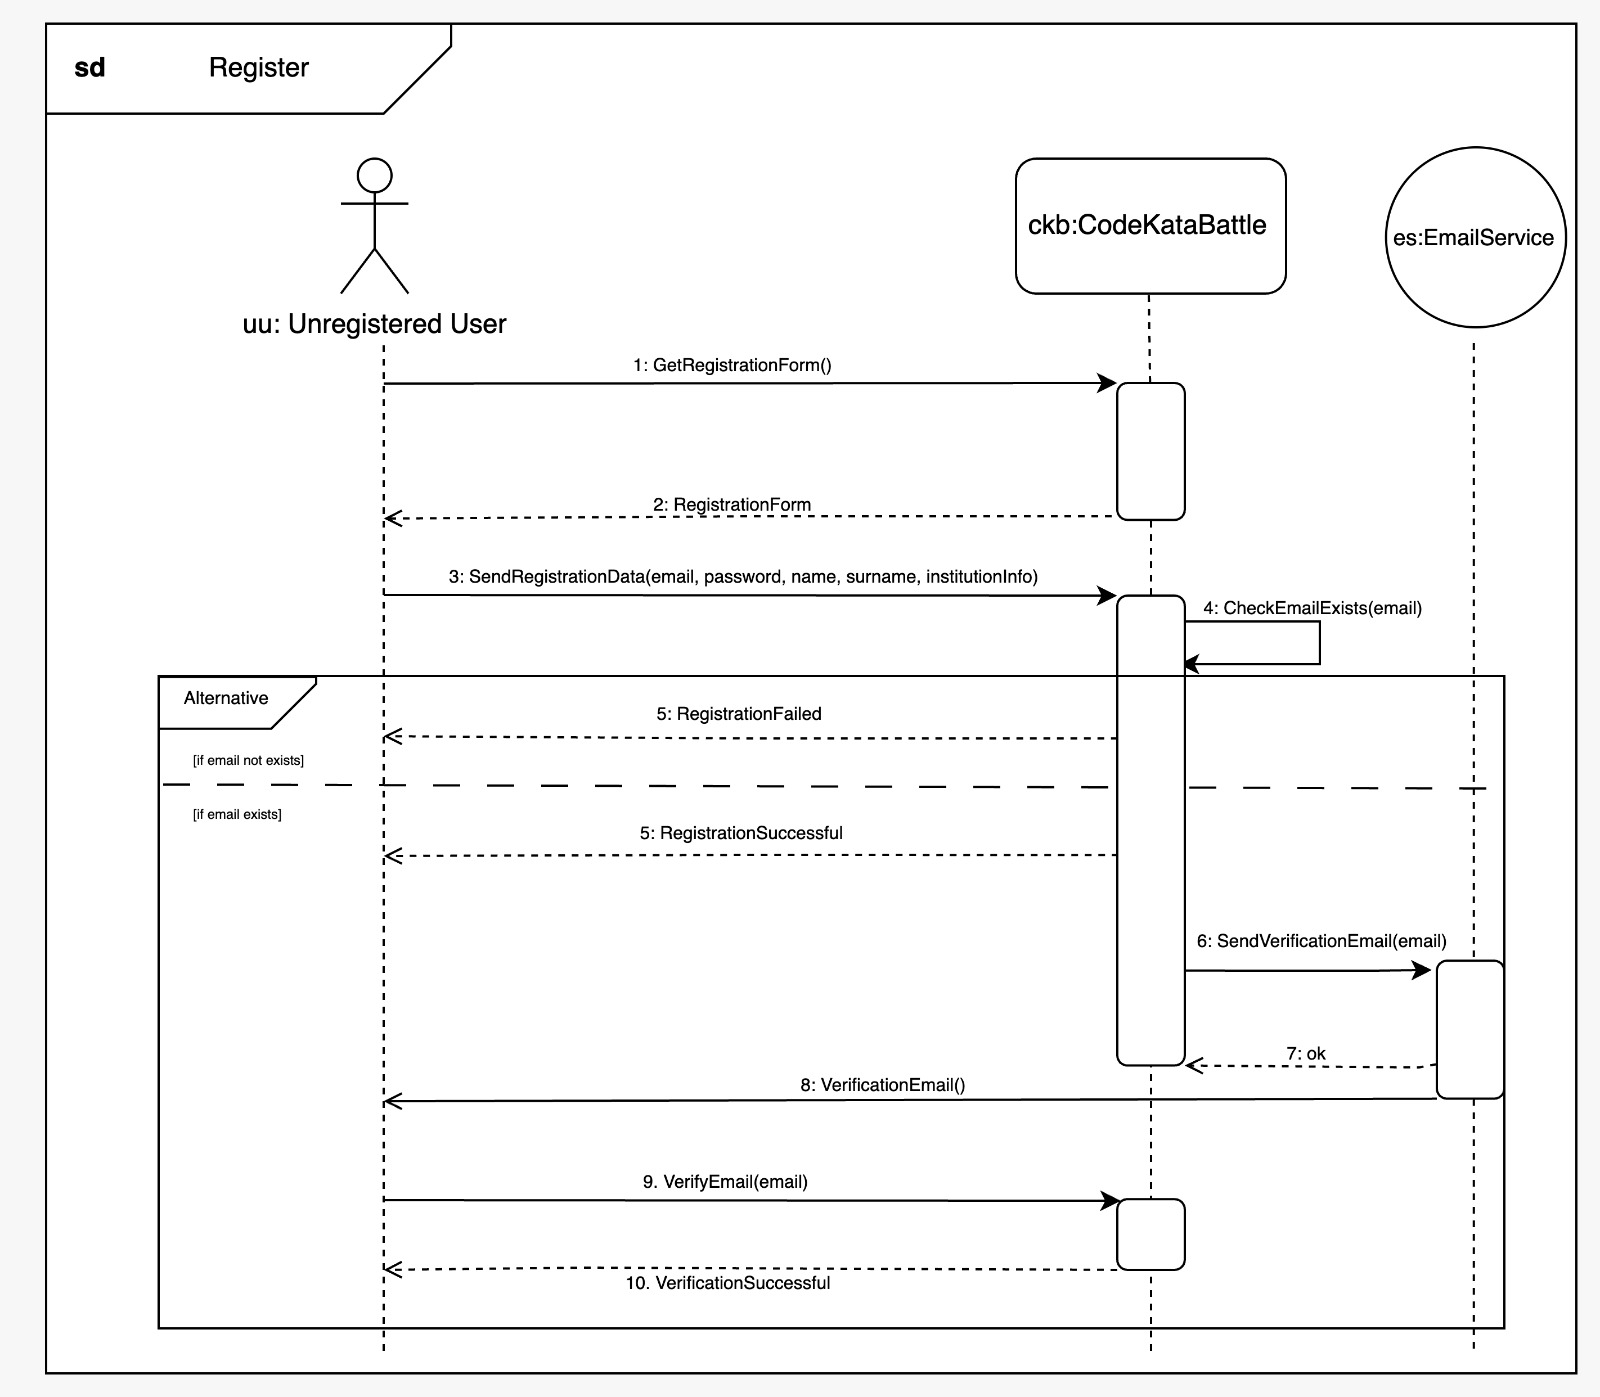
\includegraphics[scale=0.2]{Images/sequence_diagrams/SD-register.jpeg}
        \caption{$SD_{1}$ - Register}
    \end{figure}


    \item Login
    \begin{figure}[H]
        \centering
        \includegraphics[scale=0.2]{Images/sequence_diagrams/SD-login.jpeg}
        \caption{$SD_{2}$ - Login}
    \end{figure}
    
    \newpage
    \item View a Tournament
    \begin{figure}[H]
        \centering
        \includegraphics[scale=0.2]{Images/sequence_diagrams/SD-view_tournament.jpeg}
        \caption{$SD_{3}$ - View a Tournament}
    \end{figure}
    
    \item View the Tournament Leaderboard
    \begin{figure}[H]
        \centering
        \includegraphics[scale=0.2]{Images/sequence_diagrams/SD-view_tournament_leaderboard.jpeg}
        \caption{$SD_{4}$ - View the Tournament Leaderboard}
    \end{figure}
    \newpage
    \item View a Battle
    \begin{figure}[H]
        \centering
        \includegraphics[scale=0.2]{Images/sequence_diagrams/SD-view_battle.jpeg}
        \caption{$SD_{5}$ - View a Battle}
    \end{figure}
    \item View the Battle Instructions
    \begin{figure}[H]
        \centering
        \includegraphics[scale=0.2]{Images/sequence_diagrams/SD-view_battle_instructions.jpeg}
        \caption{$SD_{6}$ - View the Battle Instructions}
    \end{figure}
    \newpage
    \item View the Battle Rankings
    \begin{figure}[H]
        \centering
        \includegraphics[scale=0.2]{Images/sequence_diagrams/SD-view_battle_rankings.jpeg}
        \caption{$SD_{7}$ - View the Battle Rankings}
    \end{figure}
    \item Inspect a Submission
    \begin{figure}[H]
        \centering
        \includegraphics[scale=0.2]{Images/sequence_diagrams/SG-inspect_a_submission.jpeg}
        \caption{$SD_{8}$ - Inspect a Submission}
    \end{figure}
    \newpage
    \item Search Tournaments
    \begin{figure}[H]
        \centering
        \includegraphics[scale=0.2]{Images/sequence_diagrams/SD-search_tournaments.jpeg}
        \caption{$SD_{9}$ - Search Tournaments}
    \end{figure}
    \item Register to a Tournament
    \begin{figure}[H]
        \centering
        \includegraphics[scale=0.2]{Images/sequence_diagrams/SD-register_to_tournament.jpeg}
        \caption{$SD_{10}$ - Register to a Tournament}
    \end{figure}
    \newpage
    \item Register to a Battle
    \begin{figure}[H]
        \centering
        \includegraphics[scale=0.2]{Images/sequence_diagrams/SD-register_to_battle.jpeg}
        \caption{$SD_{11}$ - Register to a Battle}
    \end{figure}
    \newpage
    \item Complete the Team Registration for the Battle
    \begin{figure}[H]
        \centering
        \includegraphics[scale=0.2]{Images/sequence_diagrams/SD-complete_team_registration_for_battle.jpeg}
        \caption{$SD_{12}$ - Complete the Team Registration for the Battle}
    \end{figure}
    \newpage
    \item Respond to the Team Invitation
    \begin{figure}[H]
        \centering
        \includegraphics[scale=0.2]{Images/sequence_diagrams/SD-respond_to_team_invitation.jpeg}
        \caption{$SD_{13}$ - Respond to the Team Invitation}
    \end{figure}
    \item Submission
    \begin{figure}[H]
        \centering
        \includegraphics[scale=0.2]{Images/sequence_diagrams/SD-submission.jpeg}
        \caption{$SD_{14}$ - Submission}
    \end{figure}
    \newpage
    \item View Profile
    \begin{figure}[H]
        \centering
        \includegraphics[scale=0.2]{Images/sequence_diagrams/SD-view_profile.jpeg}
        \caption{$SD_{15}$ - View Profile}
    \end{figure}
    \item See Own Tournaments
    \begin{figure}[H]
        \centering
        \includegraphics[scale=0.2]{Images/sequence_diagrams/SD-view_own_tournaments.jpeg}
        \caption{$SD_{16}$ - See Own Tournaments}
    \end{figure}
    \newpage
    \item See Own Battles
    \begin{figure}[H]
        \centering
        \includegraphics[scale=0.2]{Images/sequence_diagrams/SD-view_own_battles.jpeg}
        \caption{$SD_{17}$ - See Own Battles}
    \end{figure}
    \item Delete Profile
    \begin{figure}[H]
        \centering
        \includegraphics[scale=0.2]{Images/sequence_diagrams/SD-delete_profile.jpeg}
        \caption{$SD_{18}$ - Delete Profile}
    \end{figure}
    \newpage
    \item Edit Settings
    \begin{figure}[H]
        \centering
        \includegraphics[scale=0.2]{Images/sequence_diagrams/SD-edit_settings.jpeg}
        \caption{$SD_{19}$ - Edit Settings}
    \end{figure}
    \item Create Tournament
    \begin{figure}[H]
        \centering
        \includegraphics[scale=0.2]{Images/sequence_diagrams/SD-create_tournament.jpeg}
        \caption{$SD_{20}$ - Create Tournament}
    \end{figure}
    \newpage
    \item Edit Tournament Attributes
    \begin{figure}[H]
        \centering
        \includegraphics[scale=0.2]{Images/sequence_diagrams/SD-edit_tournament_attributes.jpeg}
        \caption{$SD_{21}$ - Edit Tournament Attributes}
    \end{figure}
    \item End Tournament
    \begin{figure}[H]
        \centering
        \includegraphics[scale=0.2]{Images/sequence_diagrams/SD-end_tournament.jpeg}
        \caption{$SD_{22}$ - End Tournament}
    \end{figure}
    \newpage
    \item Respond to the Tournament Invitation
    \begin{figure}[H]
        \centering
        \includegraphics[scale=0.2]{Images/sequence_diagrams/SD-respond_to_tournament_invitation.jpeg}
        \caption{$SD_{23}$ - Respond to the Tournament Invitation}
    \end{figure}
    \newpage
    \item Create Battle
    \begin{figure}[H]
        \centering
        \includegraphics[scale=0.2]{Images/sequence_diagrams/SD-create_battle.jpeg}
        \caption{$SD_{24}$ - Create Battle}
    \end{figure}
    \newpage
    \item Edit Battle Attributes
    \begin{figure}[H]
        \centering
        \includegraphics[scale=0.2]{Images/sequence_diagrams/SD-edit_battle_attributes.jpeg}
        \caption{$SD_{25}$ - Edit Battle Attributes}
    \end{figure}
\end{enumerate}
\newpage
\subsubsection{Functional Requirements}

In this section, we organized the Functional Requirements with respect to the user types. This section will consist of four parts. \textbf{Common} will include the requirements regarding both the educators and the students. \textbf{Educator} and \textbf{Student} will include the requirements related only to their respective parts. The last part, \textbf{The Platform} will include the requirements that are not directly related to any user type but still need to be executed by the system.

\begin{itemize}
	\item Common
	\begin{enumerate}
		\item The system shall allow unregistered users to register by providing a unique email, a password, a name, a surname, and institution information.
  \item The system shall allow users who received a verification email to verify their emails.
  \item The system shall allow registered users to log in by providing an email, and a password.
  \item The system shall allow authenticated users to view all tournaments.
  \item The system shall allow authenticated users to filter the tournaments by the registration status and availability. 
  \item The system shall allow authenticated users to sort the tournaments by number of participants and number of battles in it.
  \item The system shall allow authenticated users to view a specific tournament.
  \item The system shall allow authenticated users to view the leaderboard of the tournament.
  \item The system shall allow authenticated users to view all battles in a tournament.
  \item The system shall allow authenticated users to filter the battles by group size, start date - end date, registration status, institution of the battle creator, allowed programming languages, and the battle creator.
  \item The system shall allow authenticated users to search battles by text search.
  \item The system shall allow authenticated users to view a specific battle and its instructions.
  \item The system shall allow authenticated users to view the rankings of the battle.
  \item The system shall allow authenticated users to search tournaments with text search by educators, by titles, or by institutions.
  \item The system shall allow authenticated users to manage their profiles.
  \begin{enumerate}
      \item The system shall allow authenticated users to view their profiles.
      
  \item The system shall allow authenticated users to delete their profiles unless they do not have an ongoing tournament created by themselves.

    \item The system shall allow authenticated users to view their settings.
  \item The system shall allow authenticated users to edit their settings by name, surname, password, and institution information.
  \item The system shall oblige authenticated users to enter their old password during settings editing.
  
      
  \end{enumerate}




	\end{enumerate}
	\item Educator
        \begin{enumerate}[resume]
            \item The system shall allow educators to create tournaments by providing a title, a description, and a registration deadline.
            \item The system shall allow educators to invite other educators to their tournaments during tournament creation.
            \item The system shall allow educators to edit the tournaments that they have created by providing a title, a description, and a registration deadline unless the registration deadline has not passed.
            \item The system shall allow educators to end the tournaments that they have created.
            \item The system shall allow educators to accept or reject the tournament invitation to create battles coming from other educators for a tournament.

            \item The system shall allow educators to create battles by providing a title, a description, a registration deadline, a submission deadline, the allowed languages, test cases, build scripts, minimum \& maximum group size, and the scoring criteria.
            \item The system shall oblige educators to upload test case file and build script for every allowed language in battle.
		\item The system shall allow educators to manually evaluate the submissions giving extra point between 0 and 10 after the submission deadline has passed.
            \item The system shall allow educators to edit the battles that they have created.
	\end{enumerate}



	\item Student
        \begin{enumerate}[resume]
		\item The system shall allow students to register for tournaments.
		\item The system shall allow students to register for battles in which the tournaments that they have registered for.
  \item The system shall allow students to register for battles individually.
  \item The system shall allow students to register for battles by a team having a team name.
  \item The system shall allow students to invite other students to their team during battle registration.
  \item The system shall allow students to accept or reject the team invitation coming from other students for a battle.
  \item The system shall allow students to finalize their team registration or decline it.
  
	\end{enumerate}



 \item The Platform
  \begin{enumerate}[resume]
  \item The system shall create a repository for a battle after the registration deadline for that battle has passed.
     \item The system shall pull the repository of a team following a trigger from GitHub Actions.
    \item The system shall trigger the email service to send a notification email for a newly created tournament for all registered users.
    \item The system shall trigger the email service to send an invitation email for the battle to the invitee students.
    \item The system shall trigger the email service to send a notification email including the link to the battle repository to the students registered for it.
    \item The system shall trigger the email service to send an invitation email for the tournament to the invitee educators.
     \item The system shall automatically evaluate submissions by scoring criteria.
     \begin{enumerate}
         \item The system shall score the submission with respect to test cases, and test case weight.
         \item The system shall score the submission with respect to timeliness, and timeliness weight.
         \item The system shall score the submission with respect to quality aspects, and quality aspect weight.
     \end{enumerate}
     \item The system shall utilise a Static Analysis Tool to calculate the score in terms of quality aspects.
     \item The system shall create a sandbox environment for each team for the submissions in order to run the codes.
     \item The system shall automatically update the battle score of a team after the evaluation of the submission.
     \item The system shall automatically update the battle rankings when a score is updated.
     \item The system shall automatically update the tournament leaderboard at the end of each battle.
 \end{enumerate}
 
\end{itemize}

\newpage

\subsubsection{Mapping on Goals}

\begin{table}[h!]
  \centering
  \begin{tabular}{lp{15cm}}
    \hline
    \textbf{G1} & Educators are able to prepare and manage programming exercises. \\
    \hline
    \hline
    \textbf{R1} & The system shall allow unregistered users to register by providing a unique email, a password, a name, a surname, and institution information. \\

    \textbf{R2} & The system shall allow users who received a verification email to verify their emails. \\

    \textbf{R3} & The system shall allow registered users to log in by providing an email, and a password. \\

    \textbf{R16} & The system shall allow educators to create tournaments by providing a title, a description, and a registration deadline. \\

    \textbf{R18} & The system shall allow educators to edit the tournaments that they have created by providing a title, a description, and a registration deadline unless the registration deadline has not passed \\

    \textbf{R19} & The system shall allow educators to end the tournaments that they have created. \\

    \textbf{R21} & The system shall allow educators to create battles by providing a title, a description, a registration deadline, a submission deadline, the allowed languages, test cases, build scripts, minimum \& maximum group size, and the scoring criteria. \\

    \textbf{R22} & The system shall oblige educators to upload test case file and build script for every allowed language in battle. \\

    \textbf{R24} & The system shall allow educators to edit the battles that they have created. \\

    \textbf{R32} & The system shall create a repository for a battle after the registration deadline for that battle has passed. \\

    \textbf{R34} & The system shall trigger the email service to send a notification email for a newly created tournament for all registered users. \\

        \textbf{R36} & The system shall trigger the email service to send a notification email including the link to
the battle repository to the students registered for it. \\

    \hline
    \hline
    \textbf{D1} & Educators and students have basic proficiency in using web-based platforms and are familiar with basic operations such as account creation, logging in, and navigating through a digital interface \\
    \textbf{D2} & Educators have the necessary skills to create and manage coding challenges, including the ability to correctly write problem descriptions, test cases, and understand code quality metrics. \\

    \textbf{D3} & The coding problems and challenges provided by educators are free from errors and ambiguities. \\

    \textbf{D6} & The users have access to reliable internet connectivity and devices capable of supporting the web-based CKB platform. \\
    \hline
  \end{tabular}
  \captionof{table}{Mapping on $G_{1}$}
\end{table}


\newpage

\begin{table}[h!]
  \centering
  \begin{tabular}{lp{15cm}}
    \hline
    \textbf{G2} & Educators are able to work collaboratively to create coding exercises. \\
    \hline
    \hline
    \textbf{R1} & The system shall allow unregistered users to register by providing a unique email, a password, a name, a surname, and institution information. \\

    \textbf{R2} & The system shall allow users who received a verification email to verify their emails. \\

    \textbf{R3} & The system shall allow registered users to log in by providing an email, and a password. \\

    \textbf{R16} & The system shall allow educators to create tournaments by providing a title, a description, and a registration deadline. \\

    \textbf{R17} & The system shall allow educators to invite other educators to their tournaments during tournament creation. \\

     \textbf{R20} & The system shall allow educators to accept or reject the tournament invitation to create battles
coming from other educators for a tournament. \\

    \textbf{R21} & The system shall allow educators to create battles by providing a title, a description, a registration deadline, a submission deadline, the allowed languages, test cases, build scripts, minimum \& maximum group size, and the scoring criteria. \\

    \textbf{R22} & The system shall oblige educators to upload test case file and build script for every allowed language in battle. \\

    \textbf{R24} & The system shall allow educators to edit the battles that they have created. \\

    \textbf{R32} & The system shall create a repository for a battle after the registration deadline for that battle has passed. \\

    \textbf{R34} & The system shall trigger the email service to send a notification email for a newly created tournament for all registered users. \\

    \textbf{R36} & The system shall trigger the email service to send a notification email including the link to the battle repository to the students registered for it. \\

\textbf{R37} & The system shall trigger the email service to send an invitation email for the tournament to the invitee educators. \\
    
    \hline
    \hline
    \textbf{D1} & Educators and students have basic proficiency in using web-based platforms and are familiar with basic operations such as account creation, logging in, and navigating through a digital interface \\
    \textbf{D2} & Educators have the necessary skills to create and manage coding challenges, including the ability to correctly write problem descriptions, test cases, and understand code quality metrics. \\

    \textbf{D3} & The coding problems and challenges provided by educators are free from errors and ambiguities. \\

    \textbf{D6} & The users have access to reliable internet connectivity and devices capable of supporting the web-based CKB platform. \\
    \hline
  \end{tabular}
  \captionof{table}{Mapping on $G_{2}$}
\end{table}


\newpage

\begin{table}[h!]
  \centering
  \begin{tabular}{lp{15cm}}
    \hline
    \textbf{G3} & Students are able to participate in programming exercises individually or with a team. \\
    \hline
    \hline
    \textbf{R1} & The system shall allow unregistered users to register by providing an unique email, a password, a name, a surname, and institution information. \\

    \textbf{R2} & The system shall allow users who received a verification email to verify their emails. \\

    \textbf{R3} & The system shall allow registered users to log in by providing an email, and a password. \\

    \textbf{R4} & The system shall allow authenticated users to view all tournaments. \\
     
     \textbf{R5} & The system shall allow authenticated users to filter the tournaments by the registration status and availability. \\

    \textbf{R6} & The system shall allow authenticated users to sort the tournaments by number of participants and number of battles in it. \\

    \textbf{R7} & The system shall allow authenticated users to view a specific tournament. \\

\textbf{R9} & The system shall allow authenticated users to view all battles in a tournament. \\
\textbf{R10} & The system shall allow authenticated users to filter the battles by group size, start date - end date, registration status, institution of the battle creator, allowed programming languages, and the battle creator. \\
\textbf{R11} &  The system shall allow authenticated users to search battles by text search. \\
\textbf{R12} &  The system shall allow authenticated users to view a specific battle and its instructions.\\
\textbf{R14} &  The system shall allow authenticated users to search tournaments with text search by educators, by titles, or by institutions.\\


\textbf{R25} &  The system shall allow students to register for tournaments.\\
\textbf{R26} &  The system shall allow students to register for battles in which the tournaments that they have registered for.\\
\textbf{R27} &  The system shall allow students to register for battles individually.\\
\textbf{R28} &  The system shall allow students to register for battles by a team having a team name.\\
\textbf{R29} &  The system shall allow students to invite other students to their team during battle registration.\\
\textbf{R30} &  The system shall allow students to accept or reject the team invitation coming from other students for a battle.\\
\textbf{R31} &  The system shall allow students to finalize their team registration or decline it.\\

\textbf{R35} & The system shall trigger the email service to send an invitation email for the battle to the invitee students. \\
    
    \hline
    \hline
    \textbf{D4} & Students have at least foundational knowledge in programming and can understand and respond to coding challenges.\\
    \textbf{D5} & Students’ submissions to the platform are their original work. \\
    \textbf{D6} & The users have access to reliable internet connectivity and devices capable of supporting the web-based CKB platform. \\
    \textbf{D7} & Students have familiarity with GitHub operations such as forking a repository, setting up GitHub Actions, and committing and pushing their codes.\\
    \hline
  \end{tabular}
  \captionof{table}{Mapping on $G_{3}$}
\end{table}



\newpage



\begin{table}[h!]
  \centering
  \begin{tabular}{lp{15cm}}
    \hline
    \textbf{G4} & Students are able to get evaluations for their coding solutions, enhancing their learning experience. \\
    \hline
    \hline
    \textbf{R1} & The system shall allow unregistered users to register by providing a unique email, a password, a name, a surname, and institution information. \\

    \textbf{R2} & The system shall allow users who received a verification email to verify their emails. \\

    \textbf{R3} & The system shall allow registered users to log in by providing an email, and a password. \\

    \textbf{R7} & The system shall allow authenticated users to view a specific tournament. \\

    \textbf{R8} & The system shall allow authenticated users to view the leaderboard of the tournament. \\

\textbf{R12} &  The system shall allow authenticated users to view a specific battle and its instructions.\\
\textbf{R13} &  The system shall allow authenticated users to view the rankings of the battle.\\

\textbf{R15} &  The system shall allow authenticated users to manage their profiles.\\

\textbf{R23} & The system shall allow educators to manually evaluate the submissions giving extra point between 0 and 10 after the submission deadline has passed.\\

\textbf{R25} &  The system shall allow students to register for tournaments.\\
\textbf{R26} &  The system shall allow students to register for battles in which the tournaments that they have registered for.\\

\textbf{R32} & The system shall create a repository for a battle after the registration deadline for that battle has passed.\\
\textbf{R33} & The system shall pull the repository of a team following a trigger from GitHub Actions.\\

\textbf{R38} & The system shall automatically evaluate submissions by scoring criteria.\\
\textbf{R39} & The system shall utilise a Static Analysis Tool to calculate the score in terms of quality aspects.\\

\textbf{R40} & The system shall create a sandbox environment for each team for the submissions in order to run the codes.\\
\textbf{R41} & The system shall automatically update the battle score of a team after the evaluation of the submission.\\
\textbf{R42} & The system shall automatically update the battle rankings when a score is updated. \\
\textbf{R43} & The system shall automatically update the tournament leaderboard at the end of each battle.\\


    \hline
    \hline
    \textbf{D1} & Educators and students have basic proficiency in using web-based platforms and are familiar with basic operations such as account creation, logging in, and navigating through a digital interface.\\
    \textbf{D4} & Students have at least foundational knowledge in programming and can understand and respond to coding challenges. \\
    \textbf{D5} & Students’ submissions to to platform are their original work. \\
    \textbf{D6} & The users have access to reliable internet connectivity and devices capable of supporting the web-based CKB platform. \\
    \textbf{D7} & Students have familiarity with GitHub operations such as forking a repository, setting up GitHub Actions, and committing and pushing their codes.\\
    \textbf{D8} & The automated testing and scoring systems within the CKB platform are trusted by users to fairly and accurately assess coding submissions. Similarly, educators are trusted in the case of manual evaluation of submissions.\\
    
    \hline
  \end{tabular}
  \captionof{table}{Mapping on $G_{4}$}
\end{table}



\newpage




\begin{table}[h!]
  \centering
  \begin{tabular}{lp{15cm}}
    \hline
    \textbf{G5} & Educators are able to compare students’ performance based on certain programming exercises. \\
    \hline
    \hline
    \textbf{R1} & The system shall allow unregistered users to register by providing an unique email, a password, a name, a surname, and institution information. \\

    \textbf{R2} & The system shall allow users who received a verification email to verify their emails. \\

    \textbf{R3} & The system shall allow registered users to log in by providing an email, and a password. \\

    \textbf{R7} & The system shall allow authenticated users to view a specific tournament. \\

    \textbf{R8} & The system shall allow authenticated users to view the leaderboard of the tournament. \\

\textbf{R12} &  The system shall allow authenticated users to view a specific battle and its instructions.\\
\textbf{R13} &  The system shall allow authenticated users to view the rankings of the battle.\\

\textbf{R16} &  The system shall allow educators to create tournaments by providing a title, a description, and a registration deadline.\\
\textbf{R21} &  The system shall allow educators to create battles by providing a title, a description, a registration deadline, a submission deadline, the allowed languages, test cases, build scripts, minimum \& maximum group size, and the scoring criteria.\\

\textbf{R23} &  The system shall allow educators to manually evaluate the submissions giving extra point between 0 and 10 after the submission deadline has passed.\\

\textbf{R41} & The system shall automatically update the battle score of a team after the evaluation of the submission.\\
\textbf{R42} & The system shall automatically update the battle rankings when a score is updated. \\
\textbf{R43} & The system shall automatically update the tournament leaderboard at the end of each battle.\\

    
    \hline
    \hline
    \textbf{D1} & Educators and students have basic proficiency in using web-based platforms and are familiar with basic operations such as account creation, logging in, and navigating through a digital interface.\\
    \textbf{D2} & Educators have the necessary skills to create and manage coding challenges, including the ability to correctly write problem descriptions, test cases, and understand code quality metrics. \\
    \textbf{D3} & The coding problems and challenges provided by educators are free from errors and ambiguities \\
    \textbf{D5} & Students’ submissions to the platform are their original work. \\
    \textbf{D6} & The users have access to reliable internet connectivity and devices capable of supporting the web-based CKB platform. \\
    \textbf{D7} & Students have familiarity with GitHub operations such as forking a repository, setting up GitHub Actions, and committing and pushing their codes.\\
    
    \hline
  \end{tabular}
  \captionof{table}{Mapping on $G_{5}$}
\end{table}



\newpage









\vspace{3mm}

\noindent The following subsections (\hyperref[sec:per]{3.3},\hyperref[sec:des]{3.4},\hyperref[sec:swsa]{3.5}) in \hyperref[sect:requirements]{Section 3: Specific Requirements} will include different types of \textbf{Non-Functional Requirements}. Even though they are separated into different subsections, the enumeration of elements will resume between subsections as they all represent Non-Functional Requirements. Note that constraints (i.e. Technical Requirements) are also classified as Non-Functional Requirements in this document.




\subsection{Performance Requirements}
\label{sec:per}
\begin{enumerate}
    \item The system shall respond to each user within 3 seconds for at least 90\% of the requests.
    \item The system shall support up to 1000 users concurrently.
    \item The system shall process the codes pushed to the GitHub repositories within 60 seconds unless the GitHub API is down.
\end{enumerate}
    

\subsection{Design Constraints}
\label{sec:des}
\subsubsection{Standards Compliance}
\begin{enumerate}[resume]
    \item The system shall comply with the General Data Protection Regulation (GDPR).
    \item The system shall comply with ISO/IEC 27001:2022, managing the information security.
    \item The system shall use JSON for data interchange within the APIs.
\end{enumerate}
 

\subsubsection{Hardware Limitations}
\begin{enumerate}[resume]
    \item The system requires a web-supporting device.
\end{enumerate}
 

\subsubsection{Other Constraints}
\begin{enumerate}[resume]
    \item The system user interface language shall be English.
    \item The system shall be implemented in Python \& FastAPI at the backend, and Javascript \& React at the frontend.
\end{enumerate}



\subsection{Software System Attributes}
\label{sec:swsa}
\subsubsection{Reliability}
\begin{enumerate}[resume]
    \item The system shall have a mean time between failures (MTBF) of at least 720 hours.
    \item The system shall backup at least once every 72 hours.
    \item The system shall automatically recover from minor failures within 2 minutes.
\end{enumerate}

\subsubsection{Availability}
\begin{enumerate}[resume]
    \item The system shall work 24/7 with no more than 2\% downtime, excluding scheduled maintenance.
    \item Scheduled maintenance shall be limited to a maximum of 4 hours per month, with at least a week's notice to users.
\end{enumerate}

\subsubsection{Security}
\begin{enumerate}[resume]
    \item The system shall enforce secure HTTPS connections for all data transactions.
    \item The system shall encrypt sensitive data both in transit and at rest.
\end{enumerate}

\subsubsection{Maintainability}
\begin{enumerate}[resume]
    \item The system shall support logging of all transactions and errors to facilitate debugging and maintenance.
    \item The system shall be designed to allow updates and maintenance without more than 1 hour of downtime per update.
\end{enumerate}

\subsubsection{Portability}
\begin{enumerate}[resume]
    \item The system shall be compatible with the latest versions of major web browsers including Chrome, Firefox, Safari, Opera, and Edge.
    \item The system's frontend shall be responsive and adaptable to different screen sizes, ranging from mobile devices to desktop monitors.
\end{enumerate}



